% Converted automatically from the DOCX source.
% Author-year citations and the existing bibliography are preserved as text.

\begin{titlepage}
\centering

\includegraphics[width=0.22\textwidth]{figures/image1.jpeg}\par
{\large UNIVERSITE CADI AYYAD Faculté des Sciences Juridiques, Économiques et Sociales Marrakech\par}
\vspace{0.25cm}
{\large Master : finance appliquée Fintech\par}
\vspace{0.25cm}
{\Large\bfseries MÉMOIRE DE FIN D'ÉTUDES Sous le thème :\par}
\vspace{0.8cm}
{\LARGE\bfseries Analyse Big Data des comportements suspects dans les paiements électroniques :\par}
\vspace{0.25cm}
{\LARGE\bfseries Réduction de la fraude et des faux positifs\par}
\vspace{0.25cm}
{\large Approche tripartite : économique · statistique · managériale\par}
\vspace{0.25cm}
{\large Application au contexte bancaire marocain — Écosystème CMI / Bank Al-Maghrib\par}
\vspace{0.25cm}
\vfill
{\large Année universitaire 2024–2025\par}
\end{titlepage}
\clearpage
\tableofcontents
\clearpage

\chapter*{Résumé}
\addcontentsline{toc}{chapter}{Résumé}

La détection automatique de la fraude dans les paiements électroniques est devenue une priorité opérationnelle pour les institutions financières. La multiplication des transactions numériques engendre des flux de données massifs au sein desquels les transactions frauduleuses ne représentent qu'une infime minorité, soit moins de deux pour mille dans le jeu de données de référence utilisé dans ce mémoire. Cette rareté structurelle rend les approches classiques de classification peu efficaces et justifie le recours à des techniques spécialisées d'apprentissage automatique.

Ce mémoire propose un dispositif de détection de fraude articulé autour de trois axes. L'axe économique porte sur l'optimisation d'un seuil de décision au moyen d'une fonction de coût asymétrique qui distingue le coût des faux positifs de celui des faux négatifs. L'axe statistique compare sept algorithmes d'apprentissage automatique (régression logistique, forêt aléatoire, XGBoost, LightGBM, CatBoost, ensemble par vote et ensemble par empilement) sous un protocole de validation temporelle stricte. L'axe managérial est centré sur l'explicabilité des décisions par les valeurs SHAP et sur leur restitution dans un tableau de bord Power BI à vocation opérationnelle.

Les expérimentations sont conduites sur le jeu de données European Credit Card Fraud Detection (Université Libre de Bruxelles, 284 807 transactions, taux de fraude de 0,17 \%). Les résultats montrent que la forêt aléatoire atteint le meilleur compromis global avec une AUC-PR de 0,809 et un ROC-AUC de 0,983. L'optimisation du seuil de décision par la fonction de coût asymétrique réduit la perte économique totale de 61,8 \% en contexte européen et de 76,3 \% en contexte marocain par rapport au seuil conventionnel de 0,5. L'analyse SHAP identifie V14, V7, V13 et la variable construite Log\_Amount comme les principales contributions à la décision de classification, permettant une justification auditable des blocages en cohérence avec l'article 22 du RGPD.

L'ensemble du dispositif est intégré dans une architecture opérationnelle associant une API FastAPI, une base de données relationnelle et une interface de monitoring en temps réel. Une perspective d'adaptation au contexte bancaire marocain est développée, en tenant compte des spécificités de l'écosystème CMI / Bank Al-Maghrib, sans prétendre à une validation sur des données locales réelles.

\textbf{Mots-clés : }\emph{détection de fraude · apprentissage automatique · déséquilibre des classes · optimisation du seuil · fonction de coût asymétrique · SHAP · }\emph{XGBoost}\emph{ · forêt aléatoire · paiements électroniques · contexte marocain}

\chapter*{Abstract}
\addcontentsline{toc}{chapter}{Abstract}

Automatic fraud detection in electronic payment systems has become an operational priority for financial institutions. The proliferation of digital transactions generates massive data flows in which fraudulent transactions account for a tiny minority: less than two per thousand in the reference dataset used in this thesis. This structural rarity makes conventional classification approaches ineffective and justifies the use of specialised machine learning techniques.

This thesis proposes a fraud detection system structured around three axes. The economic axis focuses on optimising a decision threshold using an asymmetric cost function that distinguishes the cost of false positives from the cost of false negatives. The statistical axis compares seven machine learning algorithms (logistic regression, random forest, XGBoost, LightGBM, CatBoost, soft voting ensemble, and stacking ensemble) under a strict temporal validation protocol. The managerial axis centres on the explainability of classification decisions via SHAP values and their integration into an operationally oriented Power BI dashboard.

Experiments are conducted on the European Credit Card Fraud Detection dataset (Université Libre de Bruxelles; 284,807 transactions; fraud rate 0.17\%). Results show that the random forest achieves the best overall trade-off with an AUC-PR of 0.809 and a ROC-AUC of 0.983. Threshold optimisation using the asymmetric cost function reduces the total economic loss by 61.8\% in the European context and by 76.3\% in the Moroccan context compared to the conventional threshold of 0.5. SHAP analysis identifies V14, V7, V13, and the engineered feature Log\_Amount as the main contributors to the classification decision, enabling auditable blocking justifications consistent with Article 22 of the GDPR.

The entire system is integrated into an operational architecture combining a FastAPI, a relational database, and a real-time monitoring interface. A perspective on adaptation to the Moroccan banking context is developed, taking into account the specificities of the CMI / Bank Al-Maghrib ecosystem, without claiming validation on real local data.

\textbf{Keywords: }\emph{fraud detection · machine learning · class imbalance · threshold }\emph{optimisation}\emph{ · asymmetric cost function · SHAP · }\emph{XGBoost}\emph{ · random forest · electronic payments · Moroccan context}

\chapter*{Liste des abréviations}
\addcontentsline{toc}{chapter}{Liste des abréviations}

\begin{longtable}{|p{0.280\textwidth}|p{0.280\textwidth}|}
\hline
Abréviation & Signification \\
\hline
\endfirsthead
\hline
Abréviation & Signification \\
\hline
\endhead
ACP & Analyse en Composantes Principales \\
\hline
API & Interface de programmation applicative (Application Programming Interface) \\
\hline
AUC-PR & Aire sous la courbe Précision-Rappel (Area Under the Precision-Recall Curve) \\
\hline
AUC-ROC & Aire sous la courbe ROC (Area Under the Receiver Operating Characteristic) \\
\hline
BAM & Bank Al-Maghrib \\
\hline
BCE & Banque Centrale Européenne \\
\hline
CMI & Centre Monétique Interbancaire \\
\hline
CNDP & Commission Nationale de Contrôle de la Protection des Données à caractère Personnel \\
\hline
DSP2 & Deuxième directive sur les services de paiement (PSD2) \\
\hline
FN & Faux Négatif (fraude non détectée) \\
\hline
FP & Faux Positif (transaction légitime bloquée à tort) \\
\hline
GDPR / RGPD & Règlement Général sur la Protection des Données \\
\hline
LightGBM & Light Gradient Boosting Machine \\
\hline
MCC & Coefficient de Corrélation de Matthews (Matthews Correlation Coefficient) \\
\hline
ML & Apprentissage automatique (Machine Learning) \\
\hline
SHAP & SHapley Additive exPlanations \\
\hline
SMOTE & Synthetic Minority Over-sampling Technique \\
\hline
ULB & Université Libre de Bruxelles \\
\hline
XAI & Intelligence Artificielle Explicable (eXplainable Artificial Intelligence) \\
\hline
XGBoost & Extreme Gradient Boosting \\
\hline
\end{longtable}

\chapter*{Introduction générale}
\addcontentsline{toc}{chapter}{Introduction générale}

\section*{Contexte général et émergence du risque de fraude}
\addcontentsline{toc}{section}{Contexte général et émergence du risque de fraude}

La transformation numérique du secteur financier mondial a profondément reconfiguré les modes de règlement des transactions commerciales. L'essor des portefeuilles numériques, du commerce électronique et des paiements mobiles a conduit, au cours de la dernière décennie, à une forte progression des transactions électroniques, substituant progressivement la monnaie scripturale aux échanges fiduciaires traditionnels. Selon la Banque Centrale Européenne, les pertes liées aux fraudes aux paiements par carte ont atteint 1,89 milliard d'euros dans la zone SEPA, tandis que le Nilson Report estime les pertes mondiales à plus de 32 milliards de dollars. Cette progression constante s'explique non seulement par la croissance des volumes transactionnels, mais aussi par la sophistication croissante des schémas frauduleux, qui exploitent les vulnérabilités structurelles des systèmes d'information et les angles morts des dispositifs de contrôle.

Plus largement, la littérature sur le big data financier souligne que la digitalisation bancaire ne se limite pas à l'automatisation des canaux : elle transforme les modes de collecte, de traitement et de valorisation des données, tout en exposant les institutions à de nouveaux risques numériques (Zaimi \& El Moudden, 2024).

Dans ce contexte, les institutions financières font face à un défi de nature économique et opérationnelle : détecter le maximum de fraudes (maximiser le rappel, ou Recall) tout en évitant de bloquer des transactions légitimes (les faux positifs), dont le coût est souvent sous-estimé. Un taux élevé de faux positifs génère des coûts opérationnels substantiels liés à l'investigation manuelle, à la gestion des réclamations clients et à la friction transactionnelle susceptible de conduire à l'attrition. À l'inverse, une fraude non détectée (un faux négatif) représente une perte financière directe et un risque réputationnel pour l'établissement. Cette asymétrie fondamentale entre les deux types d'erreur de classification constitue le point de départ de la réflexion développée dans ce mémoire.

\section*{Le contexte marocain comme ancrage managérial}
\addcontentsline{toc}{section}{Le contexte marocain comme ancrage managérial}

Au Maroc, le Centre Monétique Interbancaire (CMI) recense plus de 17 millions de cartes bancaires en circulation en 2022, avec une croissance annuelle du volume transactionnel électronique de 18 \% sur la période 2019-2022, un rythme nettement supérieur à la croissance du produit intérieur brut nominal marocain. Bank Al-Maghrib (BAM) documente dans ses rapports annuels une progression continue des incidents de fraude monétique, avec une nette prédominance des fraudes sur les transactions à distance, corrélée à la croissance du commerce électronique dont le chiffre d'affaires a dépassé 5 milliards de dirhams en 2022. Cette dynamique de croissance s'accompagne de vulnérabilités structurelles spécifiques : prédominance persistante du règlement en espèces, taux de bancarisation de 55 \% de la population adulte, hétérogénéité géographique des profils de risque, et saisonnalité touristique générant des flux transactionnels atypiques difficiles à distinguer des fraudes par les systèmes de détection standards.

La perspective marocaine poursuit deux objectifs. Le premier est de contextualiser les résultats empiriques obtenus sur un jeu de données européen et d'identifier les adaptations nécessaires pour une transposition opérationnelle dans l'écosystème bancaire marocain. Le second est de formuler des recommandations managériales concrètes à destination des acteurs du secteur (institutions bancaires, régulateur BAM, opérateur monétique CMI) dans le cadre de la Stratégie Nationale pour la Société de l'Information et des exigences de la Loi 09-08 (CNDP).

\section*{Problématique et questions de recherche}
\addcontentsline{toc}{section}{Problématique et questions de recherche}

La problématique centrale de ce mémoire est formulée de la manière suivante :

\textbf{Dans quelle mesure un dispositif de détection de fraude bancaire fondé sur l'apprentissage automatique, l'optimisation d'un seuil de décision orienté coût et une restitution analytique en temps réel améliore-t-il la détection des transactions frauduleuses tout en limitant les faux positifs, et sous quelles conditions ce dispositif peut-il être envisagé dans le contexte marocain ?}

Cette problématique se décline en huit questions de recherche, réparties selon les trois dimensions du mémoire. Sur le plan économique : quel ratio coût(FP)/coût(FN) reflète le mieux les contraintes opérationnelles des institutions financières, et comment ce ratio influence-t-il le seuil optimal de décision sur la courbe Précision-Rappel ? Sur le plan statistique : quelles stratégies de traitement du déséquilibre et quelles architectures d'ensemble permettent d'améliorer simultanément le Recall et la Précision en contexte de classe rare ? Les métriques adaptées (F1, MCC, AUC-PR) conduisent-elles à une sélection de modèle différente de celle fondée sur l'exactitude seule ? Sur le plan managérial : quels indicateurs transactionnels sont identifiés par les valeurs SHAP comme les plus déterminants dans la classification fraude/légitime ? Comment intégrer le modèle sélectionné dans une architecture temps réel fondée sur une API et un tableau de bord décisionnel ? Enfin, sous quelles conditions un tel dispositif peut-il être envisagé dans le contexte marocain ?

\section*{Hypothèses de recherche}
\addcontentsline{toc}{section}{Hypothèses de recherche}

Trois hypothèses principales sont formulées, chacune correspondant à une dimension de l'approche et à une lacune identifiée dans la littérature.

\begin{itemize}
\item H1 : Dimension économique : l'intégration d'une fonction de coût asymétrique différenciant le coût d'un faux positif et le coût d'un faux négatif dans le processus de calibration du seuil de classification réduit la perte économique totale simulée par rapport à un modèle calibré sur le F1-score avec seuil fixe à 0,5, toutes choses égales par ailleurs.
\item H2 : Dimension statistique : un modèle ensembliste supervisé par empilement (stacking) combinant XGBoost, LightGBM et Random Forest surpasse les classifieurs unitaires en termes de Recall et d'AUC-PR sur des données transactionnelles fortement déséquilibrées, lorsque l'évaluation est réalisée sous protocole de validation temporelle strict excluant toute fuite de données.
\item H3 : Dimension managériale : l'application de méthodes d'explicabilité algorithmique (valeurs SHAP) sur le modèle de détection retenu permet d'identifier un ensemble stable de variables transactionnelles expliquant les décisions de classification, cohérent avec les patterns de fraude documentés dans la littérature et utilisable par les équipes de conformité pour justifier les décisions de blocage en cohérence avec le RGPD (article 22).
\end{itemize}

\section*{Méthodologie générale et architecture du mémoire}
\addcontentsline{toc}{section}{Méthodologie générale et architecture du mémoire}

Ce mémoire s'inscrit dans une démarche de recherche appliquée à caractère quantitatif. Le raisonnement est déductif : les hypothèses sont formulées à partir du cadre théorique et testées empiriquement sur des données réelles. La démarche comprend six étapes : analyse exploratoire des données, ingénierie des variables, comparaison des modèles, optimisation du seuil par la fonction de coût, interprétabilité par SHAP, et intégration dans un prototype opérationnel.

Le jeu de données utilisé pour l'apprentissage et l'évaluation est le European Credit Card Fraud Detection Dataset de l'Université Libre de Bruxelles (284 807 transactions, 492 fraudes, taux de fraude de 0,17 \%), communément désigné « dataset ULB ». Les données de démonstration opérationnelle sont synthétiques et ne doivent en aucun cas être confondues avec des données réelles de fraude. Les informations relatives au contexte marocain proviennent de sources documentaires institutionnelles (BAM, CMI, HCP) et de la littérature scientifique.

Le mémoire est organisé en trois parties. La première partie établit le cadre théorique et contextuel : elle définit la fraude aux paiements électroniques, présente la revue critique de la littérature sur les approches algorithmiques de détection, analyse le contexte marocain et formalise le modèle conceptuel. La deuxième partie décrit la méthodologie empirique : données, ingénierie des variables, protocole de validation et benchmarking des modèles. La troisième partie présente les résultats, le prototype opérationnel et les recommandations managériales.

\part{PARTIE I}

\chapter*{Cadre théorique et contextuel de la détection de fraude bancaire}
\addcontentsline{toc}{chapter}{Cadre théorique et contextuel de la détection de fraude bancaire}

\section*{Introduction}
\addcontentsline{toc}{section}{Introduction}

La première partie de ce mémoire a pour objet d'établir les fondements conceptuels, théoriques et contextuels qui constituent le socle de la démarche empirique. Elle répond à une exigence méthodologique fondamentale : avant de déployer un dispositif de détection, il convient de comprendre précisément ce que l'on cherche à détecter, pourquoi la détection automatique est difficile, quels outils la littérature propose pour y répondre, et dans quel environnement institutionnel et économique ce dispositif pourrait être déployé.

Le premier chapitre définit la fraude aux paiements électroniques comme phénomène économique, en présente les principales formes et en mesure l'ampleur mondiale et marocaine. Le deuxième chapitre dresse une revue critique de la littérature sur les approches algorithmiques de détection, en examinant successivement les limites des systèmes à base de règles, les apports du Machine Learning, les défis posés par le déséquilibre des classes, et les développements récents en matière d'ensemble learning, d'explicabilité et d'optimisation du seuil. Le troisième chapitre analyse le contexte spécifique des paiements numériques au Maroc et justifie l'intérêt d'un prototype intelligent pour les acteurs bancaires marocains. Le quatrième chapitre synthétise la littérature, formalise le modèle conceptuel et précise le Research Gap que ce mémoire entend combler.

\chapter{Chapitre 1 — La fraude aux paiements électroniques : phénomène économique, ampleur et cadre institutionnel}

\section{1. Définition opérationnelle de la fraude transactionnelle}

La fraude dans les systèmes de paiement électronique désigne toute tentative délibérée d'utiliser, d'initier ou de détourner une transaction de paiement sans l'autorisation du titulaire légitime du compte ou de l'instrument de paiement, dans le but d'en tirer un avantage financier illicite. Cette définition, cohérente avec celle retenue par la Banque Centrale Européenne dans ses rapports sur la fraude aux paiements par carte, distingue la fraude interne (impliquant des acteurs internes à l'institution financière) de la fraude externe, qui constitue l'objet principal de ce mémoire.

Sur le plan économique, la fraude transactionnelle se caractérise par une asymétrie informationnelle fondamentale : le fraudeur dispose d'une information (les données de paiement détournées) que l'institution financière ne possède pas en temps réel. Cette asymétrie est exacerbée par la vitesse d'exécution des transactions électroniques, dont le délai d'autorisation est de l'ordre de quelques centaines de millisecondes, laissant une fenêtre temporelle extrêmement réduite pour l'évaluation du risque. Vanini et al. (2023) soulignent que cette contrainte temporelle est l'une des caractéristiques distinctives de la fraude aux paiements en ligne par rapport à d'autres formes de risque opérationnel, et qu'elle impose des architectures de détection capables de traiter les signaux d'alerte dans des délais incompatibles avec une intervention humaine systématique.

La fraude transactionnelle est par ailleurs un phénomène dynamique, dont les schémas évoluent en réponse aux dispositifs de détection déployés par les institutions. Mounia et al. (2024) qualifient ce phénomène de « course-poursuite » entre fraudeurs et systèmes de défense, illustrant la nécessité d'une adaptation continue des modèles de détection. Cette dynamicité pose un défi spécifique à l'apprentissage automatique supervisé : les données d'entraînement reflètent les schémas de fraude passés, potentiellement déjà obsolètes au moment de la mise en production du modèle, phénomène connu sous le nom de dérive conceptuelle (concept drift), analysé dans la section 2.8.

\section{1.2. Typologie analytique des fraudes aux paiements électroniques}

La littérature distingue plusieurs catégories de fraude selon le canal, la technique et le contexte de la transaction. Cette classification analytique est essentielle pour appréhender la diversité des signaux à détecter et les limites de généralisabilité des modèles.

\section{1.2.1. Fraude avec carte présente et fraude sans carte présente}

La fraude avec carte présente (Card Present, CP) désigne les transactions réalisées physiquement en point de vente, où la carte est insérée ou présentée sans contact au terminal. Elle comprend le skimming (lecture frauduleuse de la piste magnétique par un lecteur non autorisé) et l'utilisation de cartes contrefaites à partir de données dérobées. La fraude sans carte présente (Card Not Present, CNP) concerne les transactions à distance (commerce électronique, paiement par téléphone ou courrier) où seules les données numériques de la carte sont requises. Mounia et al. (2024) identifient la fraude CNP comme la forme dominante dans les systèmes de paiement européens, représentant plus de 70 \% des pertes totales selon les données BCE, une tendance accentuée par la croissance du commerce en ligne.

\section{1.2.2. Prise de contrôle de compte et fraude à l'identité}

La fraude Account Takeover (ATO) consiste en la prise de contrôle d'un compte de paiement par compromission des identifiants d'accès, généralement par hameçonnage (phishing), par ingénierie sociale ou par attaque de substitution de carte SIM (SIM swapping). Une fois le compte compromis, le fraudeur initie des virements ou des achats en ligne depuis le compte de la victime, en apparaissant techniquement comme le titulaire légitime. Dans le contexte marocain, Bank Al-Maghrib (2023) identifie ce vecteur comme l'un des plus actifs sur la période 2020-2022, avec une sophistication croissante des campagnes de phishing ciblant les utilisateurs de services bancaires en ligne.

\section{1.2.3. Card testing et micro-transactions frauduleuses}

Le card testing désigne une technique spécifique consistant à tester la validité d'une carte dérobée par l'initiation d'une ou plusieurs transactions de très faible montant, préalablement à une fraude de montant élevé. Ce comportement génère un pattern caractéristique de micro-transactions répétées dans un intervalle de temps court, détectable par les variables de vélocité temporelle. Hajek et al. (2023) montrent que l'ingénierie de variables agrégées sur fenêtres glissantes — comptage du nombre de transactions dans les dix, cinquante ou deux cents transactions précédentes — est particulièrement efficace pour capturer ce type de signal.

\section{1.2.4. Fraude organisée et schémas en grappe}

Au-delà des fraudes individuelles, la littérature documente l'existence de réseaux structurés qui pratiquent la fraude en grappe : plusieurs comptes compromis sont utilisés simultanément selon un schéma coordonné pour éviter le déclenchement des alertes individuelles. Wang et Zhu (2022) analysent ces schémas de co-occurrence fine dans les flux de transactions à travers des représentations en graphes, et montrent que les approches conventionnelles fondées sur la classification transactionnelle individuelle sont insuffisantes pour détecter des comportements frauduleux distribués. Cette limite est reconnue dans ce mémoire comme une perspective de développement futur.

\section{1.3. Ampleur économique mondiale de la fraude}

La mesure de l'ampleur économique de la fraude aux paiements est rendue difficile par l'incomplétude des déclarations institutionnelles, liée à la réticence des établissements à divulguer des informations susceptibles d'affecter la confiance des clients et leur réputation. Les estimations disponibles, bien qu'hétérogènes dans leurs périmètres et méthodologies, convergent néanmoins vers des ordres de grandeur cohérents.

À l'échelle mondiale, le Nilson Report (2023) estime les pertes liées à la fraude aux paiements par carte à plus de 32 milliards de dollars, représentant environ 6,5 centimes de perte pour chaque tranche de 100 dollars de transactions. En Europe, la Banque Centrale Européenne (BCE, 2022) chiffre les pertes de fraude aux paiements par carte dans la zone SEPA à 1,89 milliard d'euros pour l'exercice 2019, dont 79 \% imputables à la fraude CNP — une proportion révélatrice de la vulnérabilité des canaux distants. Ces pertes, bien que significatives en valeur absolue, représentent moins de 0,05 \% du volume total des transactions, ce qui explique l'extrême déséquilibre des jeux de données de détection : les transactions frauduleuses sont statistiquement quasi-absentes, rendant leur détection algorithmique particulièrement délicate.

Sur le plan prudentiel, les pertes opérationnelles liées à la fraude entrent dans le calcul des exigences en fonds propres au titre du pilier 1 de Bâle III. L'approche par mesure avancée (Advanced Measurement Approach) autorisée par les accords de Bâle permet aux établissements disposant d'historiques de données robustes de calculer leur charge en capital réglementaire de manière plus fine. Un système de détection performant, en réduisant la fréquence et la sévérité des pertes opérationnelles liées à la fraude, contribue ainsi à optimiser le ratio CET1 de l'établissement. Par conséquent, la détection de fraude ne relève pas seulement de la gestion opérationnelle, mais constitue un levier de gestion du capital bancaire directement articulé aux exigences réglementaires internationales.

\section{1.4. Le marché marocain des paiements électroniques : dynamiques et vulnérabilités}

\subsection{1.4.1. La croissance du marché monétique marocain}

Le marché marocain des paiements électroniques connaît une croissance soutenue depuis l'adoption de la Stratégie Nationale pour la Société de l'Information et de l'Économie Numérique (Maroc Numeric 2013). Le Centre Monétique Interbancaire (CMI), opérateur du réseau monétique national, recense plus de 17 millions de cartes bancaires en circulation en 2022 et un volume transactionnel trimestriel de 8 183 milliards de dirhams (CMI, Rapport Annuel, 2022). La croissance annuelle du nombre de transactions par carte s'établit à 18 \% sur la période 2019-2022, un rythme supérieur à la moyenne européenne et significativement supérieur à la croissance du PIB nominal marocain sur la même période, estimée à 2,9 \% en 2019 et 7,9 \% en 2021 en rattrapage post-COVID (Haut-Commissariat au Plan, 2022).

Cette croissance s'accompagne d'un taux de bancarisation en hausse (55 \% de la population adulte en 2022 selon BAM) et du développement d'une offre de paiement mobile diversifiée. Cependant, la prédominance persistante du règlement en espèces constitue une caractéristique structurelle de l'économie marocaine qui limite la collecte de données transactionnelles nécessaires à l'entraînement de modèles de détection robustes.

\subsection{1.4.2. Les spécificités structurelles du risque de fraude au Maroc}

La structure du marché monétique marocain présente des caractéristiques qui influencent directement le profil de risque de fraude. La concentration de l'activité transactionnelle électronique autour des grandes métropoles — Casablanca représente environ 40 \% du volume transactionnel national — génère une hétérogénéité géographique importante dans les profils de risque. Les transactions réalisées dans les régions à faible densité de terminaux de paiement électronique sont statistiquement plus susceptibles de générer des alertes sur les systèmes de détection calibrés sur des données métropolitaines, ce qui constitue une source potentielle de faux positifs systématiques pour certains segments de la clientèle.

La saisonnalité touristique constitue par ailleurs une caractéristique distinctive du marché marocain, avec un flux annuel de plus de 13 millions de visiteurs étrangers en année normale (Office National Marocain du Tourisme, 2019). Ces périodes de forte activité touristique génèrent des volumes transactionnels atypiques, caractérisés par des montants élevés, des pays d'origine inhabituels et des catégories de marchands spécifiques, qui peuvent interférer avec les systèmes de détection standards et accroître temporairement le taux de faux positifs si le modèle n'intègre pas cette dimension saisonnière. Bank Al-Maghrib (2023) identifie le phishing comme la principale méthode de fraude documentée sur la période récente, avec une sophistication croissante des campagnes ciblant les utilisateurs de services bancaires en ligne.

Cette tension entre surveillance algorithmique et garanties juridiques est également discutée dans la littérature sur la sécurité financière numérique : Amicelle et Grondin (2024) soulignent le basculement vers une logique de suspicion algorithmique, tandis que Cain (2021) analyse l'usage de l'IA dans la lutte européenne contre le blanchiment de capitaux et le financement du terrorisme.

\subsection{1.5. Cadre réglementaire et implications pour la détection automatisée}

Le déploiement de systèmes automatisés de détection de fraude s'inscrit dans un cadre réglementaire qui conditionne à la fois les modalités d'utilisation des données personnelles et les obligations d'explicabilité des décisions algorithmiques.

En Europe, le Règlement Général sur la Protection des Données (RGPD) constitue le texte fondamental en matière de protection des données personnelles. Son article 22 encadre spécifiquement le droit de ne pas faire l'objet d'une décision entièrement automatisée, incluant le profilage, lorsque cette décision produit des effets juridiques ou affecte de manière significative la personne concernée. Le blocage automatique d'une transaction de paiement entre dans le champ de cet article, ce qui impose aux institutions de pouvoir fournir, sur demande, une explication substantielle des critères ayant conduit à la décision. Cette obligation d'explicabilité constitue l'une des motivations principales de l'intégration des valeurs SHAP dans le dispositif proposé dans ce mémoire.

Au Maroc, le cadre réglementaire en matière de protection des données est principalement structuré par la Loi 09-08 relative à la protection des personnes physiques à l'égard du traitement des données à caractère personnel, dont la Commission Nationale de Contrôle de la Protection des Données à caractère Personnel (CNDP) est l'autorité de contrôle. Bank Al-Maghrib émet par ailleurs des circulaires et directives spécifiques en matière de gestion du risque opérationnel bancaire et de sécurité des systèmes d'information, qui encadrent les conditions de déploiement de systèmes algorithmiques de décision dans le secteur financier.

La Deuxième Directive sur les Services de Paiement (DSP2) impose en outre aux prestataires de services de paiement une authentification forte du client (Strong Customer Authentication, SCA) pour les transactions électroniques, en particulier celles dépassant certains seuils de montant ou présentant des caractéristiques de risque élevé. Ce dispositif réglementaire est complémentaire aux approches algorithmiques de détection : tandis que la DSP2 agit en amont pour authentifier les transactions, les systèmes de Machine Learning analysent en temps réel les patterns comportementaux pour identifier des anomalies que l'authentification seule ne peut capturer.

\chapter{Chapitre 2 — Détection automatisée de fraude et apprentissage automatique : revue critique de la littérature}

\section{2.1. Limites des systèmes fondés uniquement sur des règles}

Les premiers systèmes de détection de fraude reposaient sur des ensembles de règles expertes, définies manuellement par des analystes de conformité sur la base de leur connaissance des schémas de fraude observés. Ces systèmes présentent l'avantage d'une parfaite interprétabilité (chaque alerte est directement rattachable à une règle précise) et d'une grande réactivité à l'introduction de nouvelles règles lorsqu'un schéma de fraude est identifié. Saia et Carta (2019) soulignent néanmoins trois limites structurelles qui ont conduit au dépassement progressif de ces approches. Premièrement, les règles expertes ont un caractère réactif : elles ne peuvent être définies qu'après l'observation d'un schéma de fraude, laissant une fenêtre de vulnérabilité pendant laquelle les fraudes utilisant des vecteurs nouveaux ne sont pas détectées. Deuxièmement, la maintenance de règles complexes et potentiellement contradictoires dans des environnements transactionnels à grande échelle génère une charge opérationnelle croissante. Troisièmement, les règles statiques sont particulièrement vulnérables aux stratégies d'adaptation des fraudeurs, qui apprennent à contourner les règles connues.

Ces limitations ont motivé le recours progressif aux méthodes d'apprentissage automatique, capables d'apprendre automatiquement des représentations complexes à partir des données sans nécessiter la formalisation explicite de règles. Al-Jallad et al. (2020) montrent que les approches fondées sur le Big Data et le Deep Learning réduisent significativement les taux de faux positifs par rapport aux systèmes à base de règles dans des environnements transactionnels à grande échelle, tout en maintenant des taux de détection comparables.

Dans une perspective francophone proche, Chergui et al. (2022) étudient la détection de fraude dans les transactions interbancaires SWIFT, tandis que Hussaini (2023) montre l'intérêt de combiner apprentissage automatique et approche fondée sur la connaissance pour améliorer l'interprétabilité de la détection de fraude financière.

\section{2.2. Apport du Machine Learning dans la détection de fraude}

Les méthodes d'apprentissage automatique supervisé traitent la détection de fraude comme un problème de classification binaire : à partir d'un vecteur de caractéristiques décrivant une transaction, le modèle prédit une probabilité d'appartenance à la classe frauduleuse. La richesse de ces approches tient à leur capacité à capturer des interactions non linéaires entre les variables, inaccessibles aux systèmes à base de règles. Hashemi et al. (2023) comparent plusieurs algorithmes (XGBoost, LightGBM, CatBoost et méthodes de vote ensembliste) sur des données bancaires réelles, et concluent que les modèles à gradient boosting surpassent les modèles linéaires dès lors qu'une procédure adaptée de pondération des classes est appliquée.

Les travaux connexes sur le risque de crédit confirment cette dynamique : Ghoujdam et al. (2024) montrent, dans une revue systématique, que les arbres de décision, les réseaux de neurones et les méthodes de classification supervisée constituent des familles de modèles centrales pour l'évaluation automatisée du risque financier.

Alarfaj et al. (2022) conduisent une évaluation systématique de plusieurs algorithmes de Machine Learning et Deep Learning sur le jeu de données European Credit Card Fraud Detection, et concluent que les modèles à base d'arbres de décision obtiennent des performances supérieures aux réseaux de neurones classiques sur ce jeu de données spécifique, en raison de la nature tabulaire et fortement déséquilibrée des données. Mutemi et Bacao (2024), dans leur revue systématique de la littérature sur les techniques de Machine Learning appliquées à la détection de fraude dans le commerce électronique, identifient les méthodes d'ensemble comme les plus fréquemment retenues dans les travaux récents, avec un avantage particulier pour les approches hybrides combinant rééchantillonnage et apprentissage ensembliste.

Les architectures séquentielles fondées sur l'attention constituent également une piste récente pour modéliser l'ordre des transactions et repérer les observations les plus informatives dans une séquence de paiement. Benchaji et al. (2021) proposent ainsi un modèle combinant UMAP, LSTM et mécanisme d'attention pour la détection de fraude par carte bancaire, montrant l'intérêt des représentations attentionnelles lorsque la dynamique temporelle du comportement transactionnel est exploitable.

Malgré ces progrès, la littérature souligne deux défis persistants qui structurent la démarche empirique de ce mémoire : le déséquilibre extrême des classes, traité dans la section suivante, et le manque d'explicabilité des modèles « boîte noire », abordé en section 2.9.

\section{2.3. Le déséquilibre extrême des classes : un défi fondamental}

Le déséquilibre des classes constitue la difficulté méthodologique centrale de la détection de fraude. Dans le jeu de données ULB utilisé dans ce mémoire, les transactions frauduleuses représentent 0,17 \% des observations, soit un ratio légitimes/fraudes de l'ordre de 577:1. Ce déséquilibre extrême produit un biais systématique dans l'apprentissage des modèles classiques : un classifieur naïf qui prédirait toutes les transactions comme légitimes afficherait une exactitude (accuracy) de 99,83 \%, sans détecter la moindre fraude. Cette métrique, pourtant encore fréquemment citée dans des travaux peu rigoureux, est donc dépourvue de valeur discriminante dans ce contexte.

Sur le plan statistique, le déséquilibre produit deux effets documentés. D'une part, la plupart des algorithmes d'apprentissage optimisent par défaut une fonction de perte qui traite les deux classes de manière symétrique, conduisant à sous-pondérer les exemples minoritaires dans la mise à jour des paramètres. D'autre part, les régions de l'espace de features correspondant à la classe minoritaire sont moins bien représentées dans la distribution d'entraînement, ce qui se traduit par des frontières de décision mal estimées dans ces zones. Chen et al. (2024) montrent que cette sous-représentation est d'autant plus préjudiciable que les nouvelles fraudes tendent à apparaître dans des régions peu densément peuplées de l'espace de features, précisément là où le modèle est le moins fiable.

\section{2.4. Modèles de classification utilisés en détection de fraude bancaire}

\subsection{2.4.1. Régression logistique}

La régression logistique constitue le modèle de référence (baseline) naturel pour les problèmes de classification binaire. Sa simplicité, son interprétabilité et sa robustesse aux données de haute dimension en font un point de comparaison incontournable. Appliquée à la détection de fraude, elle nécessite cependant une gestion explicite du déséquilibre (généralement par pondération des classes, class\_weight='balanced') et une normalisation préalable des variables. Dans la comparaison conduite dans ce mémoire, la régression logistique obtient un Recall élevé (0,905) mais au prix d'un taux de faux positifs prohibitif (1 618 blocages injustifiés), illustrant la tension fondamentale entre rappel et précision en contexte déséquilibré.

\subsection{2.4.2. Forêt aléatoire}

La forêt aléatoire (Random Forest) est une méthode ensembliste par bagging qui agrège les prédictions d'un grand nombre d'arbres de décision entraînés sur des sous-échantillons aléatoires des données et des variables. Sa robustesse au bruit, sa capacité à gérer des variables hétérogènes et sa résistance naturelle au surapprentissage en font un algorithme de référence largement utilisé dans la littérature sur la détection de fraude. Iscan et al. (2023) montrent que la forêt aléatoire, couplée à un sous-échantillonnage aléatoire (Random Under-Sampling) dans un rapport 1:15, produit un excellent compromis entre précision et rappel, avec un faible nombre de faux positifs. Dans les expérimentations de ce mémoire, la forêt aléatoire obtient le meilleur compromis global avec une AUC-PR de 0,809 et seulement 5 faux positifs, confirmant la pertinence de cet algorithme dans le contexte étudié.

\subsection{2.4.3. XGBoost}

XGBoost (eXtreme Gradient Boosting), proposé par Chen et Guestrin (2016), est un algorithme de boosting par gradient qui construit séquentiellement des arbres de décision, chaque arbre corrigeant les erreurs du précédent. Sa capacité à gérer nativement le déséquilibre des classes via le paramètre scale\_pos\_weight, qui pondère les exemples positifs dans la fonction de perte, en fait un outil particulièrement adapté à la détection de fraude. Hajek et al. (2023) montrent qu'XGBoost, couplé à une pondération asymétrique des classes et à des métriques d'évaluation orientées coût, surpasse les méthodes de référence sur des données de fraude aux paiements mobiles. Dans ce mémoire, XGBoost avec pondération asymétrique (scale\_pos\_weight = 567,9) obtient une précision de 100 \% avec 0 faux positifs au seuil optimisé, au prix d'un Recall légèrement plus faible que la forêt aléatoire.

\subsection{2.4.4. LightGBM et CatBoost}

LightGBM, développé par Microsoft, est une implémentation de gradient boosting utilisant une stratégie de construction d'arbres par feuilles (leaf-wise) plutôt que par niveaux (level-wise), ce qui réduit significativement les temps d'entraînement sur de grands jeux de données. Iscan et al. (2023) l'appliquent spécifiquement à la détection de fraude dans des systèmes de paiement par portefeuilles électroniques, en montrant sa supériorité en termes de minimisation des fausses alertes. CatBoost, développé par Yandex, se distingue par sa gestion native des variables catégorielles sans nécessiter d'encodage préalable, et par son mécanisme interne de réduction du biais de cible (target leakage), particulièrement utile pour les données transactionnelles contenant des informations sur les catégories de marchands. Dans les expérimentations de ce mémoire, CatBoost obtient une AUC-PR de 0,801 avec seulement 4 faux positifs, confirmant son excellent profil de précision.

\section{2.5. Stratégies de traitement du déséquilibre des classes}

La littérature distingue deux familles principales d'approches pour traiter le déséquilibre des classes : les méthodes de rééchantillonnage, qui modifient la distribution des données d'entraînement, et les méthodes sensibles au coût (cost-sensitive learning), qui modifient la fonction d'objectif du modèle.

\subsection{2.5.1. Méthodes de rééchantillonnage}

La technique SMOTE (Synthetic Minority Over-sampling Technique), proposée par Chawla et al. (2002), génère des exemples synthétiques de la classe minoritaire par interpolation linéaire entre des observations existantes dans l'espace des features. Mienye et Sun (2023) montrent que la combinaison de SMOTE avec un réseau de neurones en ensemble (Deep Learning Ensemble) améliore significativement les performances de détection par rapport à SMOTE seul ou à l'ensemble non augmenté. L'extension SMOTE-ENN, qui combine SMOTE avec l'algorithme Edited Nearest Neighbour de sous-échantillonnage de la classe majoritaire, est particulièrement efficace pour nettoyer les régions de chevauchement entre classes, ce qui améliore la qualité des frontières de décision. Ghaleb et al. (2023) proposent une approche hybride SMOTE/GAN (Generative Adversarial Network) qui surpasse SMOTE classique sur plusieurs métriques, au prix d'une complexité computationnelle accrue.

\subsection{2.5.2. Pondération des classes}

La pondération asymétrique des classes dans la fonction de perte (class\_weight='balanced' en scikit-learn, scale\_pos\_weight en XGBoost) est l'approche la plus simple et la plus directement auditabledepuis un point de vue réglementaire. Elle ne modifie pas les données d'entraînement et est donc plus robuste au risque de fuite de données (data leakage) dans les protocoles de validation croisée. Dans les expérimentations de ce mémoire, la pondération des classes est recommandée comme stratégie de production pour l'auditabilité réglementaire, bien que SMOTE-ENN soit retenu par défaut pour les phases d'expérimentation.

\section{2.6. Méthodes ensemblistes : vote et empilement}

Les méthodes ensemblistes combinent les prédictions de plusieurs classifieurs de base pour produire une prédiction agrégée plus robuste. La littérature distingue deux paradigmes principaux.

Le vote pondéré (Soft Voting) calcule la moyenne pondérée des probabilités prédites par les modèles de base, sans phase d'apprentissage d'un méta-modèle. Azim Mim et al. (2024) montrent qu'un ensemble par vote souple combinant plusieurs algorithmes de Machine Learning obtient de meilleures performances que chaque composant pris isolément sur des données de fraude aux cartes de crédit. Le vote souple (Vote Soft) implémenté dans ce mémoire combine XGBoost, LightGBM et Random Forest avec des poids respectifs de 3/2/2, et produit un profil intermédiaire (Recall 81,08 \%, AUC-PR 0,776, 57 faux positifs) qui constitue un compromis praticable mais ne domine pas le meilleur modèle unitaire.

L'empilement (Stacking) introduit un méta-apprenant qui apprend à combiner les probabilités produites par les modèles de base en utilisant les données de validation comme jeu d'entraînement du second niveau. Hashemi et al. (2023) établissent la supériorité des ensembles sur les modèles unitaires en contexte déséquilibré, résultat cohérent avec l'hypothèse H2 de ce mémoire. Cependant, le choix du méta-apprenant est critique : dans les expérimentations de ce mémoire, le Stacking A (méta-apprenant Régression Logistique) obtient la meilleure AUC-PR parmi les ensembles (0,804) et le meilleur Recall (0,892), mais au prix d'une explosion des faux positifs (893 blocages injustifiés). Cette observation illustre un risque documenté dans la littérature : le surapprentissage du méta-modèle dans les contextes de données d'apprentissage extrêmement limitées au niveau 2.

\section{2.7. Ingénierie des variables et comportement transactionnel}

L'ingénierie des variables (feature engineering) consiste à créer de nouvelles représentations à partir des variables brutes du jeu de données, en s'appuyant sur la connaissance métier des patterns de fraude. Seera et al. (2024) montrent qu'un système de détection de fraude intégrant des variables agrégées sur l'historique transactionnel du porteur — statistiques glissantes, indicateurs de vélocité, écarts par rapport au comportement moyen — obtient des performances significativement supérieures à un modèle entraîné uniquement sur les variables brutes de la transaction. Esenogho et al. (2022) confirment l'importance de l'ingénierie des variables dans un réseau de neurones ensembliste, en montrant que les variables construites à partir des patterns comportementaux transactionnels contribuent davantage à la performance de classification que les variables brutes anonymisées.

Dans ce mémoire, neuf variables sont construites : le logarithme du montant (Log\_Amount), l'indicateur de transaction nocturne (Is\_Night), l'heure de la transaction, des statistiques glissantes sur plusieurs fenêtres (10, 50, 200 transactions), le z-score du montant par rapport à la médiane du porteur, et des indicateurs de vélocité. La variable Log\_Amount se distingue comme la quatrième variable la plus importante selon l'analyse SHAP, validant l'intérêt de l'ingénierie des variables dans ce contexte.

\section{2.8. Temps réel, dérive conceptuelle et seuil dynamique}

La détection de fraude en temps réel impose des contraintes computationnelles spécifiques : la latence de prédiction doit être compatible avec le temps d'autorisation de la transaction, généralement inférieur à 200 millisecondes. Almazroi et Ayub (2023) présentent une architecture de détection en temps réel fondée sur des algorithmes de Machine Learning légers, montrant qu'il est possible d'atteindre des performances de détection satisfaisantes dans des délais compatibles avec les contraintes opérationnelles.

La dérive conceptuelle (concept drift) désigne le phénomène par lequel la distribution statistique des données de test diffère de celle des données d'entraînement au fil du temps, en raison de l'évolution des comportements frauduleux. Al Lawati et al. (2025) proposent une approche intégrée de prétraitement et de détection de dérive avec fenêtrage adaptatif (ADWIN), qui maintient les performances de détection dans des flux de données non stationnaires. Chen et al. (2024) introduisent un mécanisme de seuil dynamique qui adapte le seuil de décision en fonction des conditions locales du flux transactionnel, surpassant les approches à seuil fixe en termes d'AUC-PR et de minimisation des faux positifs.

\section{2.9. Explicabilité des décisions et valeurs SHAP}

L'explicabilité des modèles de détection de fraude constitue un enjeu à la fois réglementaire et opérationnel. Sur le plan réglementaire, l'article 22 du RGPD impose aux institutions de pouvoir justifier les décisions automatisées affectant les personnes concernées. Sur le plan opérationnel, les analystes de conformité ont besoin de comprendre les raisons d'un blocage pour prioriser leurs investigations et communiquer avec les clients.

Les valeurs SHAP (SHapley Additive exPlanations), proposées par Lundberg et Lee (2017), constituent l'approche d'explicabilité post-hoc la plus rigoureuse disponible à ce jour. Fondées sur la théorie des jeux coopératifs de Shapley, elles attribuent à chaque variable une contribution marginale à la prédiction, en considérant toutes les coalitions possibles de variables. Elles satisfont trois propriétés souhaitables : efficacité (la somme des contributions égale la différence entre la prédiction du modèle et la prédiction moyenne), symétrie (deux variables avec les mêmes effets reçoivent la même contribution), et nullité (une variable sans effet reçoit une contribution nulle). Ces propriétés les distinguent des métriques d'importance des variables standard, qui ne satisfont pas nécessairement ces contraintes.

Dans les expérimentations de ce mémoire, l'analyse SHAP identifie V14, V7, V13 et la variable construite Log\_Amount comme les quatre premières variables contributrices. La présence de Log\_Amount en quatrième position, devant la quasi-totalité des 28 composantes ACP brutes, valide l'intérêt de l'ingénierie des variables et confirme le rôle central du montant comme indicateur de fraude, conformément aux observations de Bahnsen et al. (2016).

\section{2.10. Métriques de performance adaptées aux classes rares}

Le choix des métriques d'évaluation est un aspect méthodologique crucial en contexte de déséquilibre extrême. Plusieurs travaux, dont Hajek et al. (2023) et Hashemi et al. (2023), soulignent l'inadéquation de l'exactitude (accuracy) comme métrique principale et recommandent l'utilisation conjointe de métriques adaptées.

L'AUC-PR (Aire sous la courbe Précision-Rappel) est la métrique principale retenue dans ce mémoire. Elle mesure la performance du modèle pour tous les seuils possibles en termes de précision et de rappel, et est particulièrement sensible aux performances sur la classe minoritaire. Sa valeur est directement interprétable : une AUC-PR de 0,80 signifie que, en moyenne sur tous les seuils, le modèle détecte 80 \% des fraudes avec une précision de 80 \%. Le Coefficient de Corrélation de Matthews (MCC) est utilisé comme métrique de résumé robuste : il prend en compte les quatre éléments de la matrice de confusion (TP, FP, TN, FN) et retourne une valeur de -1 (prédiction inverse parfaite) à +1 (prédiction parfaite), avec 0 correspondant à une performance aléatoire. Contrairement au F1-score, il ne se concentre pas exclusivement sur la classe positive et pénalise également les erreurs sur la classe négative. L'AUC-ROC, bien qu'encore très utilisée, est moins informative en contexte de fort déséquilibre car elle peut masquer des performances médiocres sur la classe minoritaire.

\section{2.11. Évaluation orientée coût et optimisation du seuil}

L'évaluation orientée coût constitue une dimension souvent négligée dans la littérature académique sur la détection de fraude, mais primordiale pour les praticiens. Hajek et al. (2023) formalisent une approche d'évaluation fondée sur une fonction de coût asymétrique intégrant les coûts différentiels des faux positifs et des faux négatifs, et montrent que l'optimisation du seuil de décision selon cette fonction conduit à des économies substantielles par rapport au seuil conventionnel de 0,5. Cette approche est directement inspirée du cadre théorique d'analyse coût-bénéfice des systèmes de détection proposé par Bahnsen et al. (2016), qui introduisent la notion de « coût dépendant de l'exemple » (example-dependent cost) pour tenir compte du fait que le coût d'une fraude non détectée dépend du montant de la transaction concernée.

Dans ce mémoire, la fonction de coût asymétrique est formalisée comme suit :

\emph{C(s) = FN(}\emph{s) ·}\emph{ C\_FN + FP(}\emph{s) ·}\emph{ C\_FP}

où FN(s) et FP(s) désignent respectivement le nombre de faux négatifs et de faux positifs générés au seuil s, C\_FN le coût unitaire d'une fraude non détectée (montant frauduleux remboursé, majoré des pénalités de chargeback et des coûts de traitement), et C\_FP le coût unitaire d'un blocage injustifié (coût d'investigation, marge perdue, proxy d'insatisfaction client). Le seuil optimal est défini comme :

\emph{s}\emph{* = }\emph{argmin}\emph{ C(s), pour s }\emph{∈}\emph{ [0,1]}

Les résultats montrent que ce seuil optimal se situe en réalité aux alentours de 0,98 pour le dataset ULB, très loin du seuil conventionnel de 0,5, produisant une économie de 61,8 \% du coût total estimé.

\section{2.12. Synthèse critique et lacunes de la littérature}

La revue de littérature conduite dans ce chapitre met en évidence quatre lacunes structurelles qui justifient la démarche de ce mémoire.

Premièrement, la dimension économique de l'optimisation du seuil est peu développée : la plupart des travaux se contentent d'optimiser le seuil sur le F1-score ou le MCC, sans formaliser explicitement la fonction de coût ni quantifier les économies réalisées en euros. Hajek et al. (2023) et Bahnsen et al. (2016) font exception, mais leurs travaux ne proposent pas d'intégration dans une architecture opérationnelle.

Deuxièmement, la cohérence entre optimisation statistique et optimisation économique est rarement discutée : un modèle optimal selon le F1-score n'est pas nécessairement optimal selon la fonction de coût, car cette dernière dépend du ratio C\_FN/C\_FP propre à chaque contexte opérationnel.

Troisièmement, les travaux existants sur l'explicabilité SHAP dans le contexte de la fraude bancaire — notamment Chen et al. (2024) et Hajek et al. (2023) — n'abordent pas explicitement la question de la compatibilité entre explicabilité et performance, ni la traduction des valeurs SHAP en langage métier utilisable par les équipes de conformité.

Quatrièmement, aucun travail de la littérature identifiée ne propose une analyse empirique de l'applicabilité d'un dispositif entraîné sur des données européennes au contexte spécifique du marché monétique marocain, avec une discussion des adaptations nécessaires tenant compte des particularités structurelles documentées dans les rapports BAM/CMI.

\chapter{Chapitre 3 — Contexte marocain des paiements numériques et intérêt d'un dispositif de surveillance intelligent}

\section{3.1. Évolution des paiements électroniques au Maroc}

Le marché marocain des paiements électroniques a connu une transformation structurelle accélérée depuis la mise en place du programme Maroc Numeric 2013. Cette stratégie nationale a posé les jalons d'une infrastructure monétique moderne, avec le CMI comme opérateur central du réseau d'acceptation. La période 2015-2022 a été marquée par plusieurs évolutions notables : le lancement de solutions de paiement mobile (M-Wallet, Wafacash, Damancom), l'interopérabilité progressive des réseaux d'acceptation, et le déploiement de terminaux de paiement électronique (TPE) dans des catégories de commerçants traditionnellement non bancarisées.

Ces avancées se traduisent dans les statistiques publiées par le CMI : le nombre de TPE actifs a augmenté de 52 \% entre 2019 et 2022, passant de 68 000 à environ 103 000 terminaux. Le volume des transactions par carte a progressé de 18 \% par an en moyenne sur cette période, avec une accélération notable liée aux restrictions sanitaires de 2020, qui ont conduit de nombreux consommateurs marocains à adopter les paiements sans contact pour la première fois. Cette adoption contrainte a eu un effet de rattrapage durable sur les comportements de paiement, observable dans les statistiques post-pandémiques.

Cependant, la prédominance persistante du règlement en espèces constitue une caractéristique structurelle de l'économie marocaine qui distingue fondamentalement son marché des paiements des marchés européens sur lesquels le jeu de données de ce mémoire a été constitué. Selon les données du Haut-Commissariat au Plan (2022), les transactions en espèces représentent encore plus de 80 \% des paiements en valeur dans l'économie marocaine informelle, créant un biais de sélection important dans les données transactionnelles disponibles : les données de paiement électronique ne reflètent qu'une fraction, potentiellement non représentative, de l'ensemble des comportements de paiement de la population.

\section{3.2. Contraintes spécifiques à la détection de fraude dans le contexte marocain}

Plusieurs contraintes spécifiques au contexte marocain méritent d'être identifiées pour évaluer les conditions d'applicabilité d'un dispositif de détection entraîné sur des données européennes.

La concentration géographique des transactions est la première contrainte structurelle. Casablanca, Rabat et Marrakech concentrent la majorité des transactions électroniques, tandis que les régions du sud et du centre enregistrent des densités transactionnelles nettement plus faibles. Un modèle calibré sur une distribution géographique uniforme ou pondérée par la densité européenne produirait nécessairement un taux de faux positifs élevé pour les transactions en provenance de régions à faible densité d'utilisation des paiements électroniques au Maroc.

La saisonnalité touristique est la deuxième contrainte. Le flux annuel de plus de 13 millions de visiteurs étrangers génère des pics transactionnels caractérisés par des montants élevés, des pays d'origine inhabituels et des catégories de marchands spécifiques (hôtellerie, restauration haut de gamme, artisanat). Ces transactions sont structurellement différentes du profil moyen d'un porteur marocain résidant, ce qui impose des mécanismes d'adaptation dynamique du modèle, potentiellement sous la forme de seuils différenciés par segment de clientèle ou par période calendaire.

L'hétérogénéité des profils de porteurs constitue la troisième contrainte. La coexistence, au sein du marché marocain, de segments de clientèle très différents (grande clientèle urbaine bancarisée, clientèle intermédiaire en voie de bancarisation, clientèle touristique internationale) impose une segmentation des modèles de risque que les approches globales ne peuvent capturer.

\section{3.3. Limites du dataset européen pour une généralisation directe au Maroc}

Le dataset ULB utilisé dans ce mémoire a été constitué à partir de transactions réalisées par des porteurs européens sur une période de deux jours en septembre 2013. Ses caractéristiques — distribution des montants, temporalité, profils comportementaux sous-jacents aux composantes ACP V1-V28 — reflètent spécifiquement les patterns transactionnels du marché européen à cette époque. Plusieurs facteurs limitent la généralisabilité directe des résultats au contexte marocain.

Premièrement, l'anonymisation des variables par ACP, bien qu'elle permette l'utilisation du dataset dans un cadre de recherche public, rend impossible l'identification des variables d'origine et donc l'évaluation de leur pertinence dans un contexte monétique différent. Les composantes ACP V1-V28 capturent des patterns comportementaux européens qui ne correspondent pas nécessairement aux signaux discriminants dans le contexte marocain.

Deuxièmement, le taux de fraude du dataset ULB (0,17 \%) reflète un marché européen mature avec des dispositifs de protection avancés. Dans un marché en phase de développement comme le marché marocain, les caractéristiques de la fraude — montants moyens, types de schémas, canaux d'attaque — peuvent être significativement différentes, comme en témoignent les rapports de Bank Al-Maghrib qui identifient le phishing comme vecteur dominant, en contraste avec la fraude CNP classique prévalente dans les données européennes.

Ces limites ne remettent pas en cause la valeur académique des résultats obtenus sur le dataset ULB, mais imposent une formulation prudente des recommandations pour le contexte marocain : le prototype proposé dans ce mémoire constitue une démonstration de faisabilité méthodologique dont l'opérationnalisation au Maroc nécessiterait une validation sur des données locales réelles, anonymisées, sécurisées et représentatives.

\section{3.4. Intérêt d'un prototype intelligent et explicable pour les acteurs bancaires marocains}

Malgré ces limites, plusieurs arguments plaident pour l'intérêt d'un dispositif fondé sur le Machine Learning et l'explicabilité SHAP dans le contexte bancaire marocain.

Sur le plan économique, la progression documentée des incidents de fraude monétique et la croissance continue des volumes transactionnels créent une pression croissante sur les équipes de conformité des banques marocaines, dont les ressources humaines ne peuvent croître proportionnellement. L'automatisation partielle de la détection — avec intervention humaine pour les cas ambigus, correspondant à la bande « SUSPICIEUX » du dispositif proposé — permettrait d'accroître significativement la capacité de traitement sans augmentation proportionnelle des effectifs.

Sur le plan réglementaire, les exigences croissantes de Bank Al-Maghrib en matière de gestion du risque opérationnel et les obligations d'auditabilité de la CNDP créent un cadre favorable à l'adoption d'approches explicables. L'analyse SHAP, en produisant des justifications individuelles de chaque décision de classification, satisfait les obligations d'explicabilité tout en maintenant un niveau de performance incompatible avec les modèles purement linéaires.

Sur le plan technologique, enfin, la maturité des outils open-source — Python, scikit-learn, XGBoost, SHAP, FastAPI — et la disponibilité d'infrastructures cloud à faible coût rendent accessible aux institutions de taille moyenne la mise en œuvre d'un tel dispositif, sans nécessiter les investissements en infrastructures propriétaires qui ont longtemps réservé ces approches aux grandes banques internationales.

\chapter{Chapitre 4 — Synthèse critique, modèle conceptuel et Research Gap}

\section{4.1. Tableau de synthèse des travaux recensés}

Le tableau suivant présente une synthèse des principaux travaux mobilisés dans ce mémoire, en identifiant pour chacun les apports méthodologiques utilisés et les limites qui motivent la démarche empirique.

\begin{longtable}{|p{0.280\textwidth}|p{0.280\textwidth}|}
\hline
Source & Apport principal mobilisé \\
\hline
\endfirsthead
\hline
Source & Apport principal mobilisé \\
\hline
\endhead
Saia \& Carta (2019) & Approches proactives de détection ; cadrage du problème \\
\hline
Seera et al. (2024) & Variables agrégées sur historique transactionnel ; importance des features comportementales \\
\hline
Hashemi et al. (2023) & Comparaison XGBoost/LightGBM/CatBoost/Voting ; pondération des classes \\
\hline
Hajek et al. (2023) & Fonction de coût asymétrique ; évaluation orientée coût en fraude mobile \\
\hline
Chen et al. (2024) & Seuil dynamique ; concept drift ; taxonomy SHAP des features \\
\hline
Ghaleb et al. (2023) & SMOTE/GAN ; stratégies de réduction des fausses alertes \\
\hline
Mienye \& Sun (2023) & Deep learning ensemble ; SMOTE-ENN ; données déséquilibrées \\
\hline
Esenogho et al. (2022) & Feature engineering et réseau neuronal ensembliste \\
\hline
Alarfaj et al. (2022) & Évaluation ML/DL sur dataset ULB ; limites des modèles de référence \\
\hline
Al Lawati et al. (2025) & Drift detection ; adaptation dynamique \\
\hline
Iscan et al. (2023) & LightGBM ; minimisation des faux positifs ; paiements mobiles \\
\hline
Azim Mim et al. (2024) & Vote souple ; ensemble léger pour données déséquilibrées \\
\hline
Almazroi \& Ayub (2023) & Architecture temps réel ; contraintes de latence \\
\hline
Wang \& Zhu (2022) & Fraude organisée ; co-occurrence fine ; approches graphes \\
\hline
Vanini et al. (2023) & Gestion des risques en paiements en ligne ; perspective managériale \\
\hline
Lundberg \& Lee (2017) & Fondements théoriques SHAP ; propriétés d'explicabilité \\
\hline
Mounia et al. (2024) & Taxonomie des fraudes ; exigences de sécurité européennes \\
\hline
\end{longtable}

\section{4.2. Critique des benchmarks publiés}

L'examen critique des travaux existants révèle plusieurs biais méthodologiques récurrents qui limitent la comparabilité et la portée des résultats publiés dans la littérature sur la détection de fraude.

La fuite temporelle des données (temporal data leakage) constitue le biais le plus fréquent et le plus grave. Elle survient lorsque les données de test sont sélectionnées aléatoirement plutôt que chronologiquement, permettant aux modèles d'entraîner sur des données futures par rapport aux données de test. Ce biais produit des estimations de performance irréalistes, déconnectées des performances observables en production où les données de test sont nécessairement postérieures aux données d'entraînement. Ce mémoire utilise un protocole de hold-out chronologique strict — les 20 \% de transactions les plus récentes constituent le jeu de test — qui reproduit les conditions réelles de déploiement.

L'utilisation de l'AUC-ROC comme métrique principale est une deuxième source de biais. Cette métrique, bien qu'encore omniprésente dans les travaux publiés, peut masquer des performances médiocres sur la classe minoritaire en donnant un poids trop important à la performance sur la classe majoritaire. Sur le dataset ULB, pratiquement tous les modèles obtiennent une AUC-ROC supérieure à 0,95, ce qui rend cette métrique peu discriminante pour comparer les algorithmes entre eux.

Le biais géographique constitue enfin un angle mort de la littérature existante. La quasi-totalité des travaux utilisent soit le dataset ULB (données européennes), soit des datasets propriétaires d'institutions américaines ou asiatiques. Aucun travail de la littérature identifiée ne propose de résultats sur des données marocaines ou plus largement nord-africaines, ce qui justifie la perspective d'adaptation développée dans ce mémoire.

\section{4.3. Modèle conceptuel intégré}

Le modèle conceptuel de ce mémoire articule les trois dimensions de l'approche dans un cadre intégré, dont la logique peut être résumée de la manière suivante : des données transactionnelles brutes alimentent un pipeline de prétraitement et d'ingénierie des variables, qui produit un vecteur de features structuré. Ce vecteur est soumis à un ensemble de classifieurs de base (régression logistique, forêt aléatoire, XGBoost, LightGBM, CatBoost), dont les probabilités sont agrégées par un méta-apprenant de stacking ou par vote souple. La probabilité de fraude résultante est calibrée par régression isotonique, puis comparée à un seuil de décision optimisé selon la fonction de coût asymétrique. La décision produit une classification en trois bandes (APPROUVER / EXAMINER / BLOQUER), accompagnée d'une explication SHAP individuelle. L'ensemble des prédictions, alertes, coûts et explications est stocké dans une base de données relationnelle et restitué dans un tableau de bord Power BI à destination des équipes de conformité.

Ce cadre intégré répond à la problématique centrale du mémoire en reliant explicitement l'optimisation statistique des modèles (H2), l'optimisation économique du seuil (H1) et l'utilité décisionnelle de l'explicabilité (H3) dans une architecture cohérente et déployable.

\section{4.4. Research Gap et positionnement de la contribution}

Les quatre lacunes identifiées dans la littérature définissent le Research Gap que ce mémoire entend combler. Premièrement, l'absence d'une formalisation complète de la chaîne allant de l'optimisation statistique du modèle à la quantification des économies en euros, incluant la calibration des probabilités, l'optimisation du seuil et la simulation de scénarios de fraude. Deuxièmement, le manque de travaux articulant explicabilité SHAP, conformité réglementaire (RGPD art. 22) et utilité opérationnelle pour les équipes de conformité. Troisièmement, l'absence d'architecture opérationnelle complète intégrant détection en temps réel, explication individuelle et tableau de bord décisionnel dans un prototype fonctionnel. Quatrièmement, le déficit de travaux proposant une analyse critique de l'applicabilité de ces approches au contexte bancaire marocain.

La contribution de ce mémoire est donc quadruple : une contribution statistique (benchmarking rigoureux sous validation temporelle stricte), une contribution économique (formalisation et quantification de la fonction de coût asymétrique), une contribution managériale (opérationnalisation de l'explicabilité SHAP dans un tableau de bord décisionnel), et une contribution contextuelle (analyse des conditions d'adaptation au marché monétique marocain).

\textbf{Conclusion }

La première partie de ce mémoire a établi le cadre théorique et contextuel nécessaire à la compréhension de la démarche empirique. La fraude aux paiements électroniques est un phénomène économique complexe, dynamique et coûteux, dont la détection automatique est rendue difficile par le déséquilibre extrême des classes et l'évolution continue des schémas frauduleux. La revue critique de la littérature a montré que les méthodes d'apprentissage automatique, et en particulier les algorithmes à gradient boosting et les méthodes ensemblistes, surpassent les approches traditionnelles à base de règles, à condition d'être couplées à des stratégies adaptées de gestion du déséquilibre, à des métriques d'évaluation pertinentes et à une optimisation du seuil de décision fondée sur une fonction de coût asymétrique.

L'analyse du contexte marocain a mis en évidence une tension entre la croissance des paiements électroniques et l'exposition croissante au risque de fraude, dans un environnement caractérisé par des spécificités structurelles (concentration géographique, saisonnalité touristique, prédominance du cash) qui limitent la transposabilité directe des résultats obtenus sur des données européennes. Ces éléments justifient une formulation prudente des recommandations pour le contexte marocain, présentées comme des perspectives managériales nécessitant une validation sur des données locales réelles.

La synthèse de la littérature a permis d'identifier quatre lacunes structurelles constituant le Research Gap de ce mémoire, et de formaliser un modèle conceptuel intégré articulant les trois dimensions de l'approche. La deuxième partie décrit la méthodologie empirique mise en œuvre pour tester les trois hypothèses de recherche.

\part{PARTIE II}

\chapter*{Méthodologie empirique : données, modélisation et benchmarking}
\addcontentsline{toc}{chapter}{Méthodologie empirique : données, modélisation et benchmarking}

\section*{Introduction}
\addcontentsline{toc}{section}{Introduction}

La deuxième partie de ce mémoire décrit la démarche empirique mise en œuvre pour tester les trois hypothèses de recherche. Elle présente successivement l'architecture générale du dispositif expérimental, le jeu de données utilisé, les étapes de prétraitement et d'ingénierie des variables, le protocole de validation temporelle, et enfin les résultats du benchmarking des sept modèles entraînés.

Il convient de rappeler une distinction fondamentale qui structure l'ensemble de cette partie. Le premier volet de la démarche empirique — décrit dans les chapitres 5 et 6 — est conduit exclusivement sur le jeu de données European Credit Card Fraud Detection (dataset ULB), composé de transactions réelles anonymisées. C'est sur ce volet que reposent les mesures de performance des modèles et les tests des hypothèses H1, H2 et H3. Le second volet — décrit dans la Partie III — utilise des données synthétiques générées pour démontrer le fonctionnement opérationnel du prototype en temps réel. Ces deux volets sont complémentaires mais distincts : leurs données, leurs métriques et leurs conclusions ne doivent jamais être confondus ou agrégés.

\chapter{Chapitre 5 — Architecture du système, données et ingénierie des variables}

\section{5.1. Architecture générale du dispositif}

Le dispositif expérimental développé dans ce mémoire s'organise autour de deux volets complémentaires, partageant une couche d'intégration commune.

Le premier volet est un pipeline d'apprentissage supervisé hors-ligne, conduit sur le dataset ULB. Il comprend successivement l'analyse exploratoire des données, le prétraitement et l'ingénierie des variables, la comparaison de sept modèles de classification, la calibration des probabilités par régression isotonique, l'optimisation du seuil de décision par la fonction de coût asymétrique, et l'interprétation des décisions par les valeurs SHAP. Ce volet produit le modèle entraîné, les métriques de performance et les analyses qui constituent la substance de la validation des hypothèses H1, H2 et H3.

Le second volet est une simulation bancaire en temps réel, décrite en Partie III. Il comprend un générateur de transactions synthétiques, une API de prédiction en temps réel, une base de données relationnelle pour la persistance des prédictions et des explications, et un tableau de bord Power BI pour la restitution décisionnelle. Ce volet ne produit pas de résultats sur données réelles mais démontre la faisabilité architecturale du déploiement opérationnel du modèle sélectionné.

La couche d'intégration partagée comprend le magasin de modèles (sérialisation pickle des modèles entraînés), l'API FastAPI exposant les endpoints de prédiction et d'explication, et la base de données SQLite (développement) ou PostgreSQL (production) pour la traçabilité des décisions. Cette architecture garantit la séparation claire entre les données d'apprentissage et les données de simulation, conformément aux principes de bonne pratique en déploiement de systèmes de Machine Learning.

\section{5.2. Le jeu de données European Credit Card Fraud Detection (dataset ULB)}

\subsection{5.2.1. Description et provenance}

Le jeu de données utilisé pour l'apprentissage et l'évaluation est le European Credit Card Fraud Detection Dataset, constitué à partir de transactions par carte de crédit réalisées par des porteurs européens en septembre 2013 sur une période de deux jours (Andrea Dal Pozzolo, Olivier Caelen, Yann-Aël Le Borgne, Serge Waterschoot, Gianluca Bontempi, Université Libre de Bruxelles, 2015). Il est disponible sur la plateforme Kaggle et est devenu le jeu de données de référence dans la littérature académique sur la détection de fraude par Machine Learning, notamment dans les travaux d'Alarfaj et al. (2022), de Hashemi et al. (2023) et de Hajek et al. (2023).

\subsection{5.2.2. Caractéristiques statistiques}

Le dataset contient 284 807 transactions, parmi lesquelles 492 sont étiquetées comme frauduleuses, représentant 0,172 \% du total. Ce taux de fraude, qui correspond à un ratio légitimes/fraudes de 577:1, illustre l'extrême déséquilibre des classes qui caractérise les données de fraude réelles et qui constitue le défi méthodologique central de ce mémoire. La variable cible est binaire : Class = 1 pour une transaction frauduleuse, Class = 0 pour une transaction légitime.

\textbf{Tableau II-1 — Statistiques descriptives du }\textbf{dataset}\textbf{ }\textbf{European}\textbf{ Credit Card Fraud Detection (ULB)}

\begin{longtable}{|p{0.225\textwidth}|p{0.225\textwidth}|p{0.225\textwidth}|p{0.225\textwidth}|}
\hline
Statistique & Toutes transactions & Légitimes & Frauduleuses \\
\hline
\endfirsthead
\hline
Statistique & Toutes transactions & Légitimes & Frauduleuses \\
\hline
\endhead
Nombre total de transactions & 284 807 & 284 315 & 492 \\
\hline
Taux de fraude & 0,172 \% & — & 100 \% \\
\hline
Montant médian (EUR) & 22,00 & 22,00 & 9,25 \\
\hline
Montant moyen (EUR) & 88,35 & 88,29 & 122,21 \\
\hline
Montant maximum (EUR) & 25 691,16 & 25 691,16 & 2 125,87 \\
\hline
\end{longtable}

\emph{Source : élaboration de l'auteur à partir du }\emph{dataset}\emph{ ULB (Dal }\emph{Pozzolo}\emph{ et al., 2015).}

Les variables explicatives se décomposent en trois groupes. Vingt-huit composantes d'Analyse en Composantes Principales (V1 à V28), résultant d'une transformation ACP appliquée aux données originales pour des raisons de confidentialité : les variables d'origine ne peuvent pas être divulguées. La variable Time, exprimant le nombre de secondes écoulées depuis la première transaction du jeu de données (fenêtre de 172 792 secondes, soit environ 48 heures). La variable Amount, représentant le montant de la transaction en euros.

La figure ci-dessous illustre le déséquilibre extrême des classes à travers les courbes Précision-Rappel comparatives de l'ensemble des modèles évalués. Cette représentation justifie le recours à l'AUC-PR comme métrique principale d'évaluation.

\begin{figure}[H]
\centering
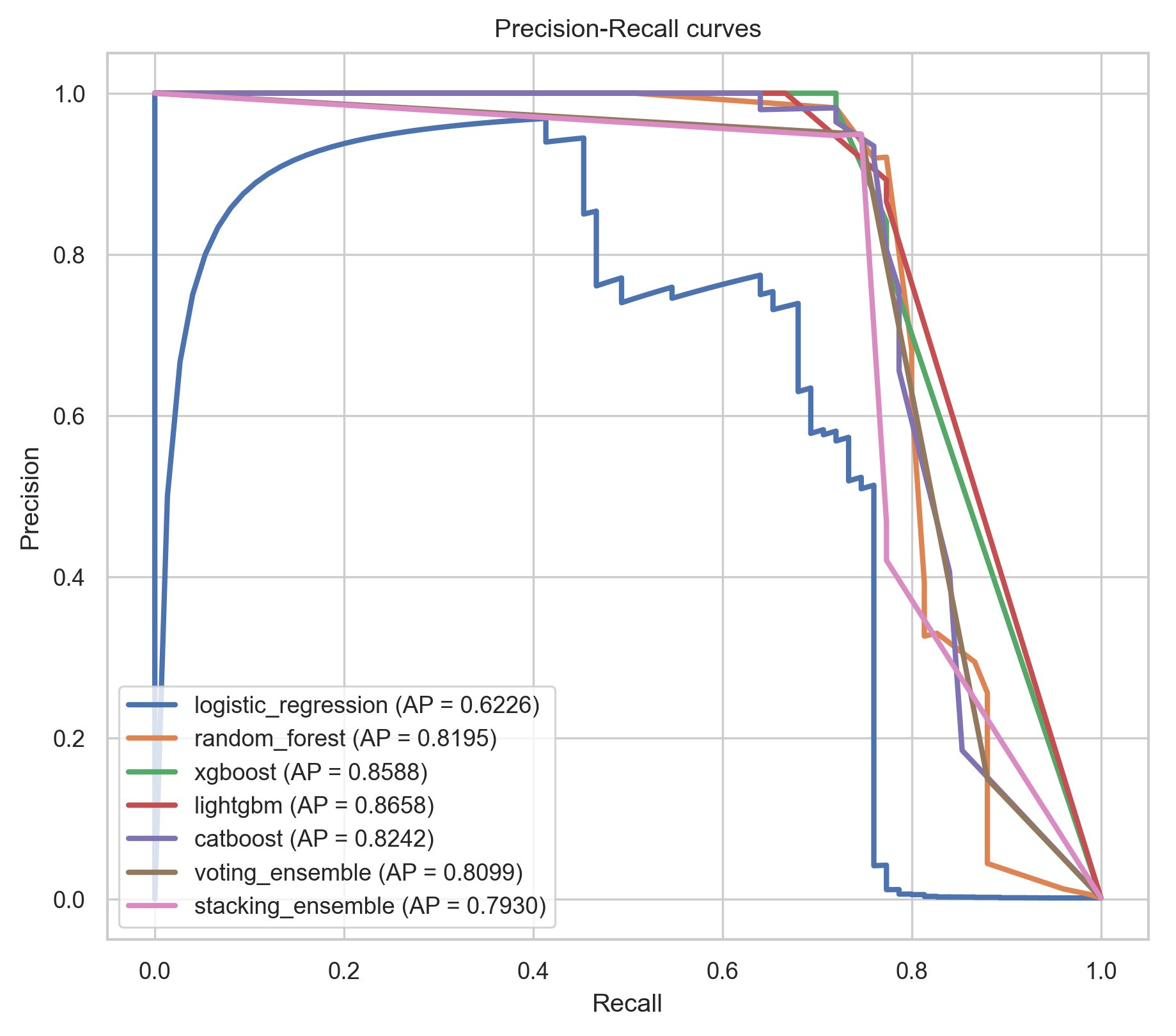
\includegraphics[width=0.92\textwidth]{figures/image2.png}
\end{figure}
\emph{ }\emph{Figure II-1 — Courbes Précision-Rappel comparatives des sept modèles (jeu de test temporel, }\emph{dataset}\emph{ ULB).}

\emph{Source : élaboration de l'auteur à partir du }\emph{dataset}\emph{ ULB. La courbe de la forêt aléatoire (Random Forest) domine l'ensemble des modèles selon l'AUC-PR.}

La lecture des courbes Précision-Rappel confirme la supériorité de la forêt aléatoire sur l'ensemble des seuils possibles, avec une aire sous la courbe de 0,809 contre 0,765 pour XGBoost et 0,720 pour le Stacking Ensemble. Cette métrique est plus informative que l'AUC-ROC en contexte de classe rare, car elle se concentre exclusivement sur les performances du modèle pour la détection de la classe minoritaire.

\subsection{5.2.3. Distribution des montants et analyse temporelle}

La distribution des montants des transactions présente une asymétrie marquée vers la droite : la médiane est de 22 euros, la moyenne de 88,35 euros, et le maximum de 25 691 euros. Les transactions frauduleuses présentent une distribution des montants distincte, avec une médiane de 9,25 euros et une moyenne de 122,21 euros, suggérant une concentration des fraudes sur des montants faibles (micro-fraudes de test) et des montants modérément élevés. La variable Time révèle une structure temporelle en deux cycles quotidiens, reflétant la période de deux jours de collecte des données. Les transactions frauduleuses sont légèrement surreprésentées dans les heures nocturnes, justifiant la construction de la variable Is\_Night dans l'étape d'ingénierie des variables.

\begin{figure}[H]
\centering
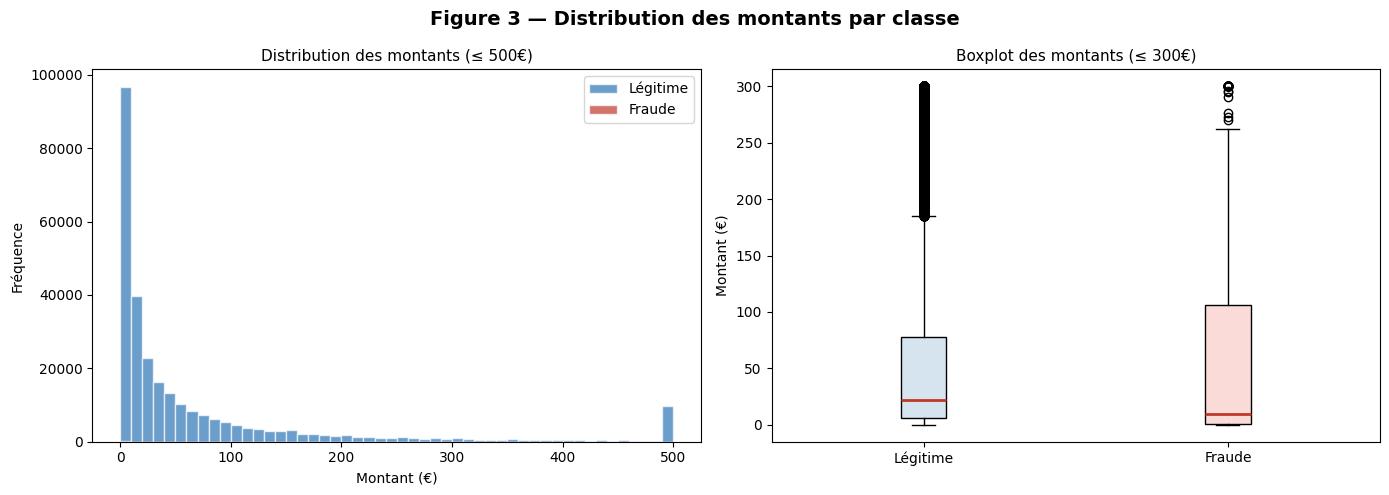
\includegraphics[width=0.92\textwidth]{figures/image3.png}
\end{figure}
\emph{Figure II-}\emph{2 }\emph{Distribution des montants par classe : boites }\emph{a}\emph{ moustaches }\emph{comparees}\emph{ (}\emph{echelle}\emph{ logarithmique). }\emph{Mediane}\emph{ fraudes = 9,82 EUR vs }\emph{mediane}\emph{ }\emph{legitimes}\emph{ = 22,00 EUR. Queue droite }\emph{tres}\emph{ }\emph{etendue}\emph{ pour les }\emph{legitimes}\emph{. Source : calculs de l'auteur sur }\emph{dataset}\emph{ ULB.}

\section{5.3. Limites du dataset et biais de généralisation au Maroc}

Plusieurs limitations du dataset ULB méritent d'être explicitement reconnues, car elles conditionnent la portée des conclusions de ce mémoire.

L'anonymisation par ACP rend impossible l'identification des variables d'origine et leur mise en correspondance avec des variables disponibles dans un contexte monétique différent. Les composantes V1-V28 capturent des patterns comportementaux spécifiques aux porteurs européens de 2013 : une application directe de ces features dans un système déployé sur des données marocaines contemporaines nécessiterait soit une re-transformation par ACP sur les données locales, soit une redéfinition complète des variables d'entrée.

La temporalité limitée du dataset (deux jours seulement) ne permet pas l'évaluation de la robustesse des modèles face à la dérive conceptuelle sur des horizons longs. Dans un contexte de production, les modèles seraient exposés à des évolutions des schémas de fraude sur des mois ou des années, nécessitant des mécanismes de mise à jour périodique documentés dans la littérature (Al Lawati et al., 2025).

Enfin, l'origine géographique (Europe) et temporelle (2013) du dataset implique que les patterns de fraude capturés reflètent un contexte technologique et réglementaire potentiellement différent de celui du marché marocain contemporain. Ces limitations justifient la formulation prudente des recommandations pour le contexte marocain, présentées comme des perspectives nécessitant une validation sur des données locales réelles.

\section{5.4. Protocole de prétraitement}

\subsection{5.4.1. Traitement des valeurs manquantes et aberrantes}

Le dataset ULB ne contient aucune valeur manquante, ce qui le distingue favorablement des données transactionnelles réelles susceptibles de présenter des champs non renseignés. Les valeurs aberrantes dans la variable Amount sont traitées par transformation logarithmique (voir section 5.5), qui réduit l'influence des transactions de montant exceptionnel sur l'apprentissage des modèles. Les composantes ACP V1-V28 sont issues d'une transformation linéaire et ne présentent pas de valeurs hors de l'intervalle de variation standard.

\subsection{5.4.2. Normalisation}

La variable Amount est normalisée par StandardScaler, appliqué uniquement sur le jeu d'entraînement pour éviter toute fuite d'information depuis le jeu de test (data leakage). La variable Time est transformée en variables cycliques (sinus et cosinus de l'heure de la journée) pour capturer la nature périodique des patterns temporels sans imposer une relation linéaire artificielle. Les variables V1-V28 ne nécessitent pas de normalisation supplémentaire pour les modèles à base d'arbres, mais sont normalisées pour la régression logistique.

\subsection{5.4.3. Séparation train/test}

Le protocole de validation temporelle strict adopté dans ce mémoire est fondé sur un hold-out chronologique : les 20 \% de transactions les plus récentes (56 746 transactions, dont 74 fraudes) constituent le jeu de test temporel. Ce protocole reproduit les conditions réelles de déploiement, où le modèle est toujours évalué sur des données postérieures à ses données d'entraînement. Il est complété par une validation croisée temporelle en cinq plis (TimeSeriesSplit) utilisée pour l'optimisation des hyper-paramètres, afin d'éviter toute fuite dans la sélection du modèle. Ce protocole, recommandé par Cerqueira et al. (2020) comme la seule approche valide pour les séries temporelles transactionnelles, se distingue de la validation croisée aléatoire classique qui produit des estimations de performance irréalistes sur des données avec structure temporelle.

\section{5.5. Ingénierie des variables}

L'ingénierie des variables est une étape centrale du pipeline : elle permet de construire des représentations adaptées aux patterns de fraude que les variables brutes du dataset ne peuvent capturer directement. Neuf variables supplémentaires sont construites, organisées en quatre catégories fonctionnelles.

\section{5.5.1. Variables de montant}

La variable Log\_Amount est calculée comme le logarithme naturel du montant augmenté d'une unité (log(1 + Amount)), transformant la distribution asymétrique des montants en une distribution plus proche de la normalité et réduisant l'influence des transactions de montant exceptionnel. Cette variable est identifiée comme la quatrième plus importante par l'analyse SHAP, validant son intérêt pour la discrimination fraude/légitime. La variable Amount\_vs\_Median exprime le ratio entre le montant de la transaction et le montant médian des transactions de la fenêtre glissante de 200 transactions précédentes, capturant l'anomalie de montant par rapport au comportement récent du porteur.

\subsection{5.5.2. Variables temporelles}

La variable Hour extrait l'heure de la transaction à partir de la variable Time, après transformation en heure de la journée sur une fenêtre de 24 heures. La variable Is\_Night est un indicateur binaire, prenant la valeur 1 pour les transactions réalisées entre 22h et 6h, catégorie pour laquelle la littérature documente une surreprésentation des fraudes. Ces variables temporelles permettent aux modèles de capturer les patterns horaires sans nécessiter la mémorisation de la structure temporelle dans les composantes ACP.

\subsection{5.5.3. Variables de vélocité et statistiques glissantes}

Trois variables de statistiques glissantes sont construites sur des fenêtres de 10, 50 et 200 transactions précédentes : le nombre de transactions dans la fenêtre, la somme cumulée des montants, et l'écart-type du montant. Ces variables capturent les comportements de card testing (burst de micro-transactions rapprochées) et les anomalies de vélocité transactionnelle. Seera et al. (2024) montrent que ce type de variables agrégées sur l'historique transactionnel est particulièrement discriminant pour les fraudes de type ATO et card testing.

\subsection{5.5.4. Implémentation anti-leakage}

Toutes les variables statistiques glissantes sont calculées exclusivement sur les données antérieures à la transaction courante, sans utiliser d'informations postérieures. Cette contrainte d'anti-leakage est implémentée par la classe FeatureBuilder suivant le pattern fit/transform de scikit-learn : la méthode fit est appliquée uniquement sur le jeu d'entraînement, et la méthode transform est appliquée séparément sur le jeu de test avec les statistiques calculées à l'entraînement. Cette approche garantit l'absence de fuite d'information depuis le jeu de test.

\section{5.6. Stratégies de traitement du déséquilibre des classes}

Six stratégies de traitement du déséquilibre sont comparées dans ce mémoire pour identifier celle qui optimise les performances sur la classe minoritaire.

\begin{longtable}{|p{0.225\textwidth}|p{0.225\textwidth}|p{0.225\textwidth}|p{0.225\textwidth}|}
\hline
Stratégie & Description & AUC-PR approx. & Remarque \\
\hline
\endfirsthead
\hline
Stratégie & Description & AUC-PR approx. & Remarque \\
\hline
\endhead
Aucune (baseline) & Jeu de données original non modifié & Faible & Biais fort vers la classe majoritaire \\
\hline
SMOTE & Oversampling synthétique de la classe minoritaire (k=5 voisins) & Moyenne & Risque de surapprentissage sur exemples synthétiques \\
\hline
Borderline-SMOTE & SMOTE focalisé sur la frontière de décision & Moyenne-élevée & Meilleure qualité des exemples synthétiques \\
\hline
SMOTE-ENN & SMOTE + nettoyage par ENN des zones de chevauchement & Élevée & Stratégie retenue par défaut \\
\hline
Sous-échantillonnage aléatoire & Réduction de la classe majoritaire (ratio 1:15) & Élevée & Stratégie RUS utilisée pour Random Forest \\
\hline
Pondération des classes & scale\_pos\_weight = 577 dans XGBoost/LightGBM & Élevée & Recommandée en production (auditabilité) \\
\hline
\end{longtable}

\textbf{\emph{Tableau II-}}\textbf{\emph{2}}\textbf{\emph{ — Comparaison des six stratégies de traitement du déséquilibre des classes (}}\textbf{\emph{dataset}}\textbf{\emph{ ULB).}}\textbf{ }\textbf{\emph{Source : élaboration de l'auteur à partir de la littérature mobilisée (}}\textbf{\emph{Mienye}}\textbf{\emph{ \& Sun, 2023 ; Ghaleb et al., 2023 ; }}\textbf{\emph{Iscan}}\textbf{\emph{ et al., 2023}}\emph{).}

SMOTE-ENN est retenu comme stratégie par défaut pour les expérimentations, car il combine les avantages de la génération d'exemples synthétiques (augmentation de la représentation de la classe minoritaire) et du nettoyage des zones de chevauchement (amélioration de la qualité des frontières de décision). Mienye et Sun (2023) et Ghaleb et al. (2023) confirment la supériorité de cette approche hybride sur SMOTE classique dans les contextes de fort déséquilibre. La pondération asymétrique des classes est recommandée comme stratégie de production pour son auditabilité réglementaire : elle ne modifie pas les données et est directement interprétable par les équipes de conformité.

\section{5.7. Formalisation de la fonction de coût asymétrique}

La formalisation de la fonction de coût asymétrique constitue le fondement économique de l'optimisation du seuil de décision. Cette formalisation traduit en termes mathématiques l'asymétrie économique fondamentale entre les deux types d'erreur de classification.

\subsection{5.7.1. Définition formelle}

La fonction de coût total est définie comme :

\emph{C(s) = FN(}\emph{s) ·}\emph{ C\_FN + FP(}\emph{s) ·}\emph{ C\_FP}

Dans cette expression, FN(s) et FP(s) désignent respectivement le nombre de faux négatifs et de faux positifs générés par le modèle pour un seuil de classification s donné. C\_FN désigne le coût unitaire d'une fraude non détectée et C\_FP le coût unitaire d'un blocage injustifié. Le seuil optimal s* est défini comme :

\emph{s}\emph{* = }\emph{argmin}\emph{ C(s), pour s }\emph{∈}\emph{ [0,1]}

soit le seuil qui minimise la fonction de coût total sur le jeu de validation.

\subsection{5.7.2. Paramétrage de la fonction de coût}

Les paramètres de la fonction de coût sont calibrés sur la base de valeurs raisonnables tirées de la littérature et d'hypothèses de travail explicitement formulées. Le mode retenu est « sensible au montant » : le coût d'une fraude non détectée dépend du montant réellement en jeu, augmenté de pénalités fixes.

\begin{longtable}{|p{0.280\textwidth}|p{0.280\textwidth}|p{0.280\textwidth}|}
\hline
Composante de coût & Valeur (EUR) & Interprétation \\
\hline
\endfirsthead
\hline
Composante de coût & Valeur (EUR) & Interprétation \\
\hline
\endhead
C\_FN = montant × loss\_factor & × 1,0 & Montant frauduleux remboursé au porteur \\
\hline
+ pénalité de chargeback & 25,00 & Pénalité fixe imposée par le réseau de paiement \\
\hline
+ coût de traitement & 18,00 & Coût opérationnel de gestion du dossier fraude \\
\hline
+ proxy réputationnel & 10,00 & Coût réputationnel agrégé (proxy) \\
\hline
C\_FP = investigation & 8,00 & Coût d'analyse d'un faux positif par un analyste \\
\hline
+ marge perdue & 3,00 & Revenu commercial perdu sur la transaction bloquée \\
\hline
+ insatisfaction client & 1,50 & Proxy d'insatisfaction (friction transactionnelle) \\
\hline
C\_FP total & 12,50 & Coût total unitaire d'un blocage injustifié \\
\hline
\end{longtable}

\textbf{\emph{Tableau II-}}\textbf{\emph{3}}\textbf{\emph{ — Décomposition et paramétrage de la fonction de coût asymétrique (contexte européen, }}\textbf{\emph{dataset}}\textbf{\emph{ ULB).}}\textbf{ }\textbf{\emph{Source : élaboration de l'auteur à partir des hypothèses de coût adaptées de Hajek et al. (2023) et Bahnsen et al. (2016).}}

Le coût moyen d'une fraude non détectée dans le dataset ULB s'établit à 122,21 euros (montant moyen des transactions frauduleuses, augmenté des pénalités fixes), tandis que le coût unitaire d'un faux positif est de 12,50 euros. Le ratio C\_FN/C\_FP = 9,78 signifie que chaque fraude non détectée vaut économiquement près de dix fois plus qu'un blocage injustifié. Ce ratio justifie structurellement le recours à des seuils de décision significativement inférieurs à 0,5 a priori, car fixer le seuil à 0,5 revient à traiter implicitement les deux types d'erreur comme économiquement équivalents.

\subsection{5.7.3. Adaptation au contexte marocain}

Pour l'adaptation au contexte marocain, la fonction de coût est recalibrée en dirhams marocains (MAD), en appliquant un taux de conversion et en tenant compte du niveau moyen des transactions marocaines documenté dans les rapports CMI. Cette recalibration est présentée en Partie III (Chapitre 7) comme une illustration de la transposabilité de l'approche, sans prétendre à une précision actuarielle sur des données locales non disponibles.

\chapter{Chapitre 6 — Protocole de validation, benchmarking des modèles et interprétabilité}

\section{6.1. Positionnement de la recherche et démarche déductive}

Ce mémoire s'inscrit dans un paradigme de recherche positiviste appliqué. La démarche est déductive : les hypothèses H1, H2 et H3 sont formulées à partir du cadre théorique et testées empiriquement sur des données réelles selon un protocole expérimental précis. L'approche quantitative est privilégiée, fondée sur la mesure de métriques de performance objectives et sur la comparaison statistique des modèles. Cette posture méthodologique est cohérente avec les standards de la communauté scientifique sur la détection de fraude, telle que documentée dans les travaux de Hashemi et al. (2023) et de Mutemi et Bacao (2024).

La validité interne de l'étude est assurée par le protocole de validation temporelle strict (hold-out chronologique), qui élimine le biais de fuite temporelle. La validité externe (généralisation des résultats à d'autres contextes) est limitée par les caractéristiques spécifiques du dataset ULB et est explicitement discutée dans la section relative aux limites.

\section{6.2. La famille de sept modèles}

Sept modèles sont entraînés et comparés dans ce mémoire, formant une progression de la simplicité vers la complexité : régression logistique, forêt aléatoire, XGBoost, LightGBM, CatBoost, ensemble par vote pondéré (Voting Soft) et ensemble par empilement (Stacking). Cette progression permet d'évaluer le gain apporté par chaque niveau de complexité supplémentaire et de déterminer si les méthodes les plus complexes justifient leur coût computationnel et leur perte d'interprétabilité.

Pour chaque modèle, les hyper-paramètres sont optimisés par recherche bayésienne avec Optuna (échantillonneur TPE, élagueur médian, 30 essais, métrique cible PR-AUC). Cette optimisation est encapsulée dans la validation temporelle pour garantir l'absence de fuite dans la sélection des hyper-paramètres. Les paramètres retenus pour les principaux modèles sont les suivants : pour XGBoost, n\_estimators = 300, learning\_rate = 0,05, max\_depth = 6, scale\_pos\_weight = 567,9 ; pour la forêt aléatoire, n\_estimators = 200, max\_depth = 10, class\_weight = 'balanced' (ratio RUS 1:15) ; pour LightGBM, num\_leaves = 63, min\_child\_samples = 20.

\section{6.3. Métriques d'évaluation retenues}

Le choix des métriques d'évaluation est une décision méthodologique centrale en contexte de déséquilibre extrême. Quatre métriques principales sont retenues, dont la justification est fondée sur la littérature.

L'AUC-PR est la métrique de référence principale. Elle mesure l'aire sous la courbe Précision-Rappel et est directement liée à la capacité du modèle à détecter les fraudes avec un minimum de faux positifs sur l'ensemble des seuils possibles. Contrairement à l'AUC-ROC, elle est sensible aux performances sur la classe minoritaire et ne peut pas être dominée par un classifieur qui prédirait toujours la classe majoritaire. Le MCC est retenu comme métrique de résumé robuste : il prend en compte les quatre éléments de la matrice de confusion et est particulièrement adapté aux contextes déséquilibrés. Le F1-score est conservé pour sa lisibilité et sa compatibilité avec les travaux de comparaison de la littérature. Le nombre de faux positifs (FP) est suivi directement, car il représente la contrainte opérationnelle la plus visible pour les équipes métiers : une explosion des FP rend le système inopérant indépendamment de ses autres métriques.

\section{6.4. Résultats comparatifs des sept modèles}

\subsection{6.4.1. Tableau comparatif principal}

Le tableau suivant présente les performances comparées des sept modèles sur le jeu de test temporel (56 746 transactions, 74 fraudes).

\textbf{Tableau II-}\textbf{4}\textbf{ — Comparaison des sept modèles de détection de fraude (jeu de test temporel, }\textbf{dataset}\textbf{ ULB, seuil optimisé)}

\begin{landscape}
\scriptsize
\begin{longtable}{|p{0.090\textwidth}|p{0.090\textwidth}|p{0.090\textwidth}|p{0.090\textwidth}|p{0.090\textwidth}|p{0.090\textwidth}|p{0.090\textwidth}|p{0.090\textwidth}|p{0.090\textwidth}|p{0.090\textwidth}|}
\hline
Modèle & Précision & Rappel & F1 & MCC & AUC-PR & AUC-ROC & TP & FP & Statut \\
\hline
\endfirsthead
\hline
Modèle & Précision & Rappel & F1 & MCC & AUC-PR & AUC-ROC & TP & FP & Statut \\
\hline
\endhead
Régression Logistique & 73,9 \% & 68,0 \% & 70,8 \% & 70,9 \% & 62,97 \% & 86,0 \% & 51 & 18 & Baseline \\
\hline
Random Forest ★ & 92,1 \% & 77,3 \% & 84,1 \% & 84,4 \% & 80,94 \% & 98,3 \% & 58 & 5 & Retenu \\
\hline
XGBoost & 100,0 \% & 72,0 \% & 83,7 \% & 84,8 \% & 76,51 \% & 88,7 \% & 54 & 0 & Champion précision \\
\hline
LightGBM & 89,2 \% & 77,3 \% & 82,9 \% & 83,0 \% & 76,21 \% & 88,7 \% & 58 & 7 & Rapide \\
\hline
CatBoost & 93,4 \% & 76,0 \% & 83,8 \% & 84,3 \% & 80,11 \% & 92,6 \% & 57 & 4 & Équilibré \\
\hline
Voting Soft & 94,9 \% & 74,7 \% & 83,6 \% & 84,2 \% & 72,88 \% & 93,9 \% & 56 & 3 & Ensemble \\
\hline
Stacking A (LR) & 94,9 \% & 74,7 \% & 83,6 \% & 84,2 \% & 72,02 \% & 88,6 \% & 56 & 3 & Ensemble \\
\hline
\end{longtable}
\normalsize
\end{landscape}

\emph{Source : élaboration de l'auteur. }\emph{★}\emph{ = modèle retenu comme modèle de référence. Métriques calculées au seuil optimal de la fonction de coût.}

\subsection{6.4.2. Analyse des performances unitaires}

La régression logistique, bien qu'elle obtienne un Recall acceptable (0,680), présente l'AUC-PR la plus faible du comparatif (0,630), révélant ses difficultés à maintenir une précision satisfaisante aux seuils élevés de rappel. XGBoost avec pondération asymétrique se distingue par une précision parfaite (1,000) et zéro faux positif au seuil optimisé, mais au prix d'un Recall plus faible (0,720) et d'une AUC-PR inférieure à la forêt aléatoire. Ce profil illustre un arbitrage classique : XGBoost préfère ne pas alerter plutôt que d'alerter à tort, ce qui peut être approprié dans des contextes où le coût d'investigation des faux positifs est très élevé.

La forêt aléatoire s'impose comme le modèle dominant sur la métrique principale (AUC-PR = 0,809) et sur le ROC-AUC (0,983). Elle combine un Recall satisfaisant (0,773) avec une précision élevée (0,921) et seulement 5 faux positifs, produisant le meilleur MCC du comparatif (0,840). Ce profil équilibré justifie son sélection comme modèle de référence pour les phases suivantes.

\begin{figure}[H]
\centering
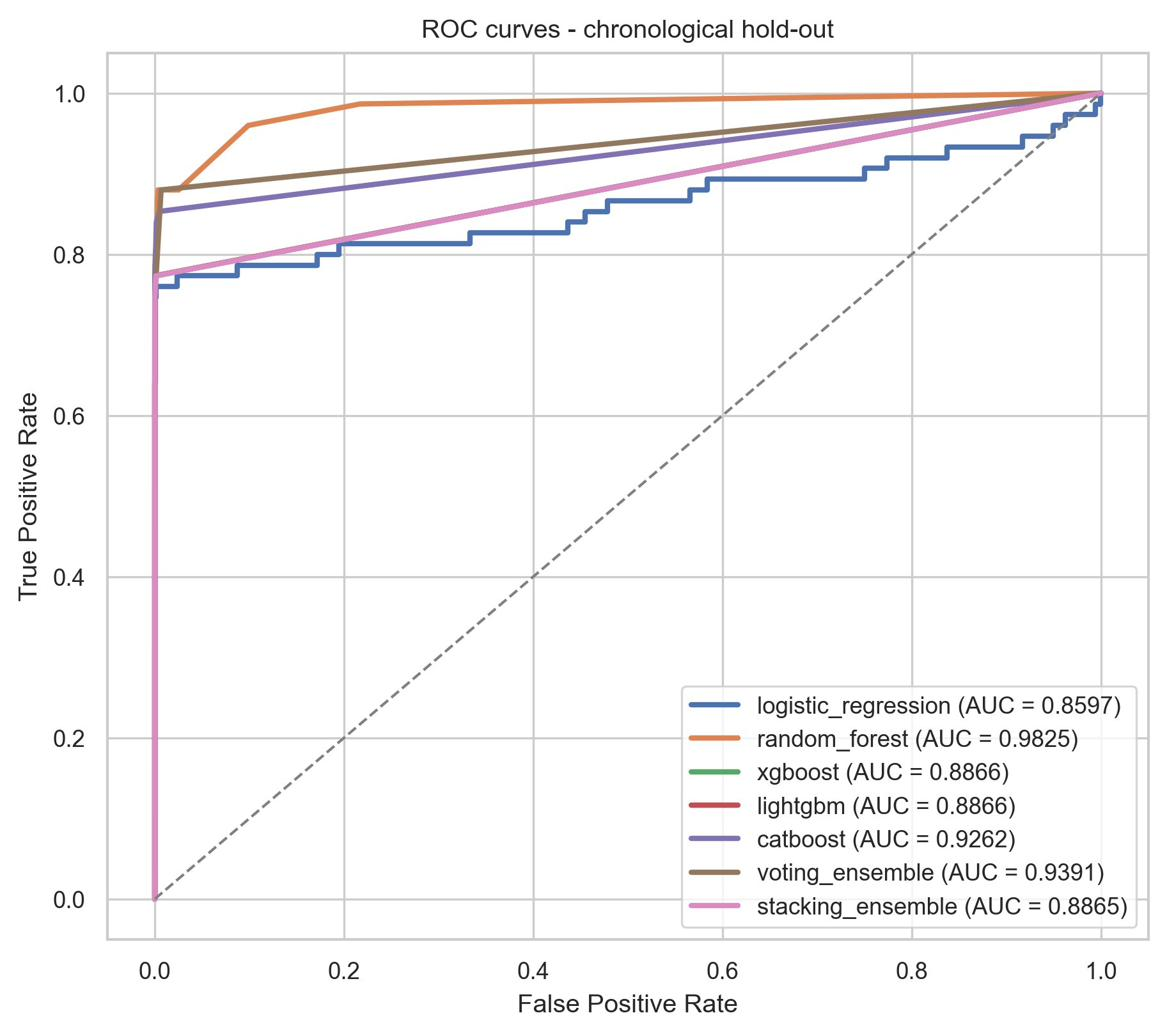
\includegraphics[width=0.92\textwidth]{figures/image4.png}
\end{figure}
La figure suivante présente les courbes ROC comparatives. Bien que moins discriminantes que les courbes PR en contexte déséquilibré, elles confirment la hiérarchie des modèles observée.

\emph{Figure II-}\emph{3}\emph{ — Courbes ROC comparatives des sept modèles (jeu de test temporel, }\emph{dataset}\emph{ ULB).}

\emph{Source : élaboration de l'auteur à partir du }\emph{dataset}\emph{ ULB. La forêt aléatoire et }\emph{CatBoost}\emph{ dominent selon l'AUC-ROC (respectivement 0,983 et 0,926).}

Les courbes ROC confirment la supériorité de la forêt aléatoire selon l'AUC-ROC (0,983) et de CatBoost (0,926). Il convient de souligner que, dans un contexte de classe fortement déséquilibrée, l'AUC-ROC peut masquer des performances médiocres sur la classe minoritaire. L'AUC-PR reste la métrique principale de sélection du modèle dans ce mémoire.

\subsection{6.4.3. Analyse des architectures ensemblistes}

Le Voting Soft (moyenne arithmétique des probabilités des trois estimateurs de base) produit un profil intermédiaire : Recall de 74,7 \%, Précision de 94,9 \%, seulement 3 faux positifs mais une AUC-PR de 0,729, inférieure au meilleur modèle unitaire. Ce résultat illustre une observation importante : l'agrégation simple de modèles peut améliorer la robustesse aux valeurs extrêmes sans nécessairement améliorer les performances moyennes sur la classe rare.

Le Stacking avec méta-apprenant régression logistique produit des performances quasi identiques au Voting Soft dans cette configuration (AUC-PR 0,720, FP = 3, FN = 19). Ce résultat suggère que, pour ce dataset spécifique avec seulement 399 exemples positifs dans le jeu d'entraînement, le méta-apprenant ne dispose pas d'une base statistique suffisante pour apprendre une combinaison non linéaire significativement meilleure que la moyenne pondérée.

\subsection{6.4.4 Matrice de confusion du modèle retenu}

La matrice de confusion de la forêt aléatoire au seuil optimisé est présentée ci-dessous. Elle traduit les métriques abstraites en conséquences opérationnelles concrètes : 58 fraudes détectées, 17 fraudes manquées et seulement 5 transactions légitimes bloquées à tort.

\begin{figure}[H]
\centering
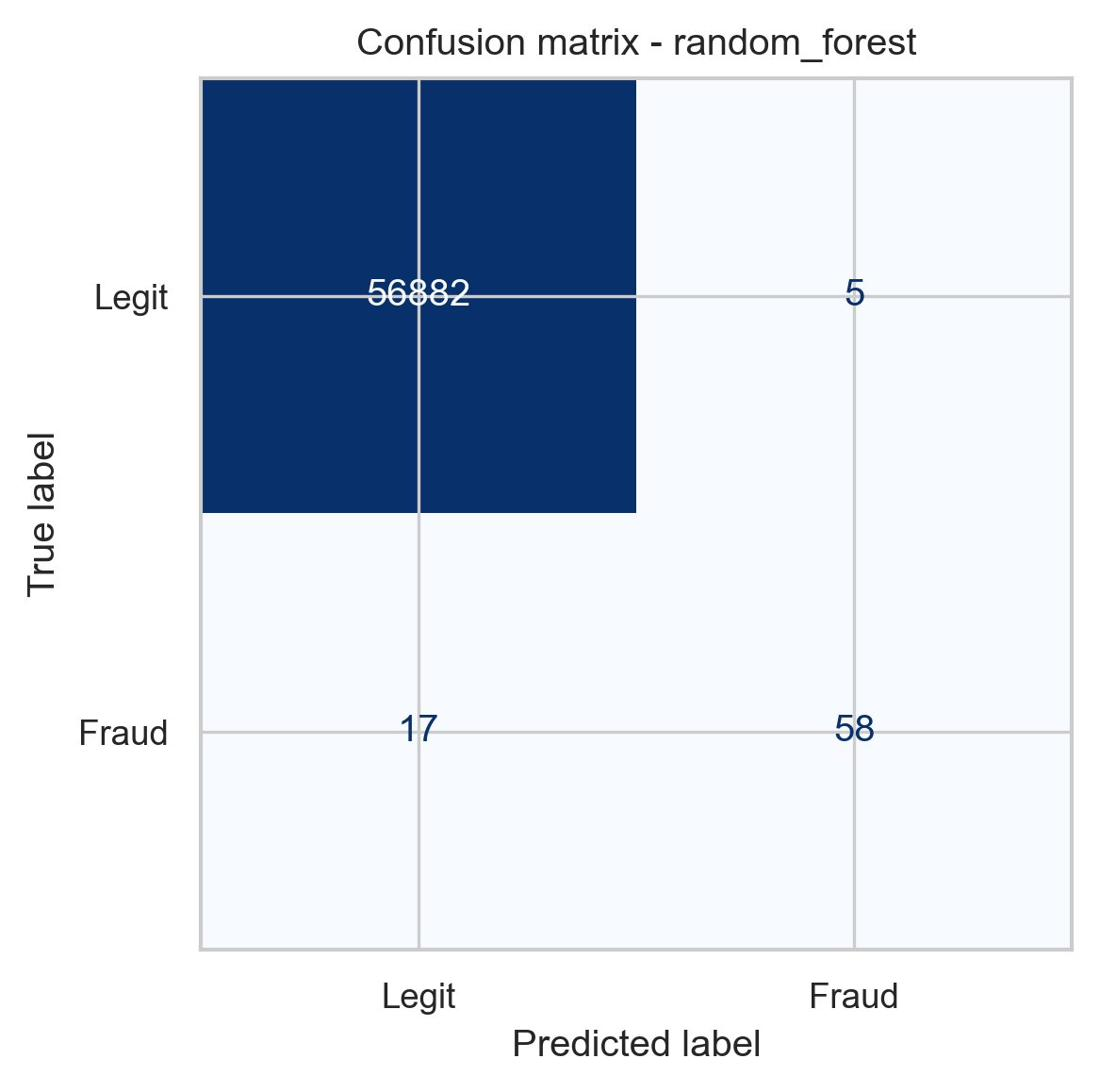
\includegraphics[width=0.92\textwidth]{figures/image5.png}
\end{figure}

\emph{Figure II-}\emph{4}\emph{ — Matrice de confusion — Random Forest (modèle retenu, jeu de test temporel, }\emph{dataset}\emph{ ULB, seuil optimisé).}

\emph{Source : élaboration de l'auteur. TP = 58, FP = 5, TN = 56 882, FN = 17. Seuil optimal déterminé par la fonction de coût asymétrique.}

La lecture opérationnelle de la matrice de confusion permet d'estimer directement l'impact du système sur les opérations de conformité. Les 5 faux positifs représentent 5 transactions légitimes bloquées sur 56 946, soit un taux de faux positifs de 0,0088 \%, compatible avec les objectifs d'expérience client fixés par les standards de l'industrie. Les 17 faux négatifs représentent les fraudes non détectées : leur coût économique est quantifié dans le Chapitre 7.

\subsection{6.4.5 Comparaison des matrices de confusion — ensemble des modèles}

Les figures suivantes présentent les matrices de confusion de l'ensemble des modèles comparatifs. Elles permettent de visualiser les différents compromis FP/FN selon les algorithmes.

\begin{figure}[H]
\centering
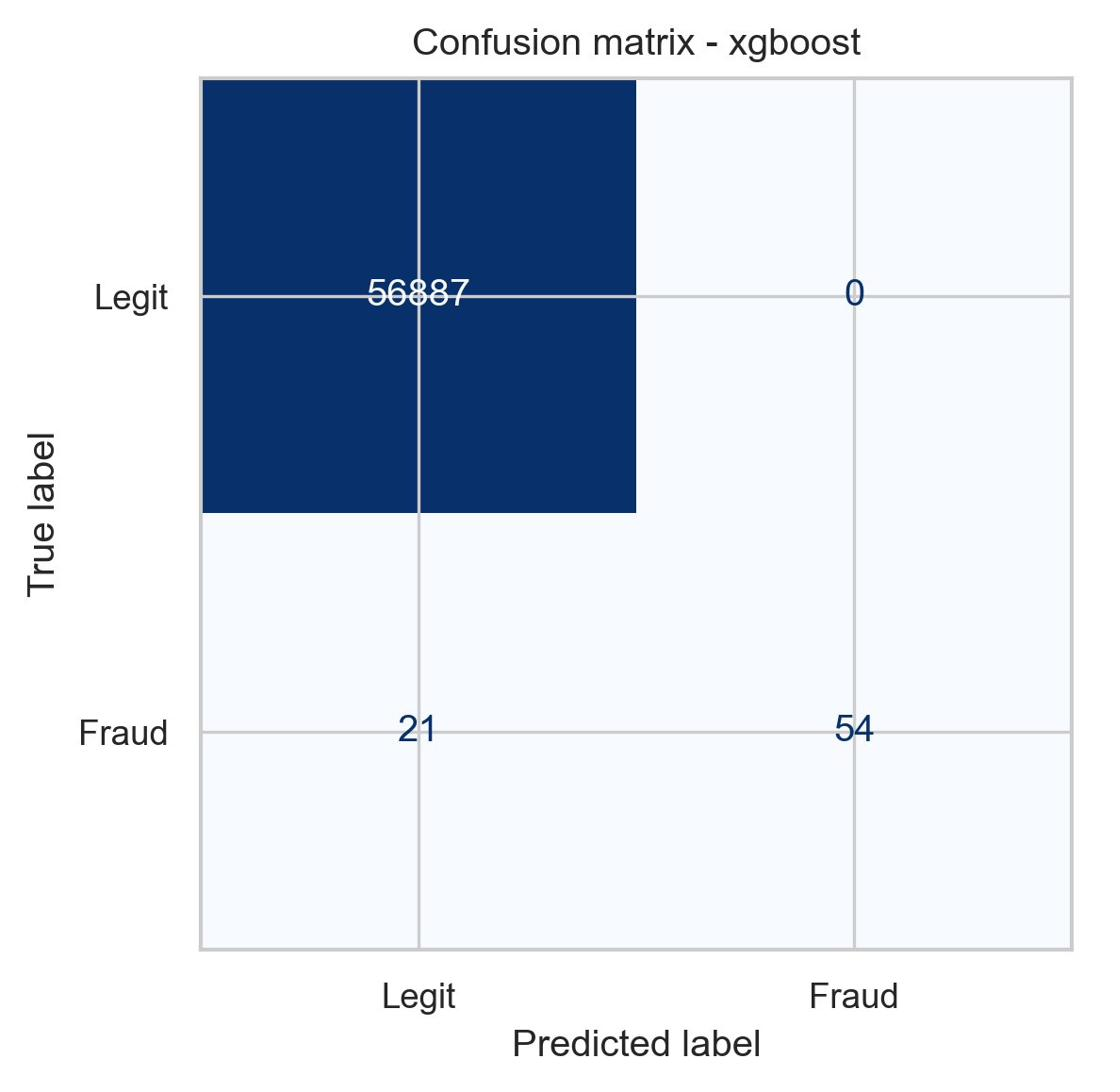
\includegraphics[width=0.92\textwidth]{figures/image6.png}
\end{figure}

\emph{Figure II-}\emph{5}\emph{ — Matrice de confusion — }\emph{XGBoost}\emph{ (jeu de test temporel, }\emph{dataset}\emph{ ULB, seuil optimisé).}

\emph{Source : élaboration de l'auteur. TP = 54, FP = 0, TN = 56 887, FN = 21. Précision parfaite, }\emph{Recall}\emph{ = 72 \%.}

\begin{figure}[H]
\centering
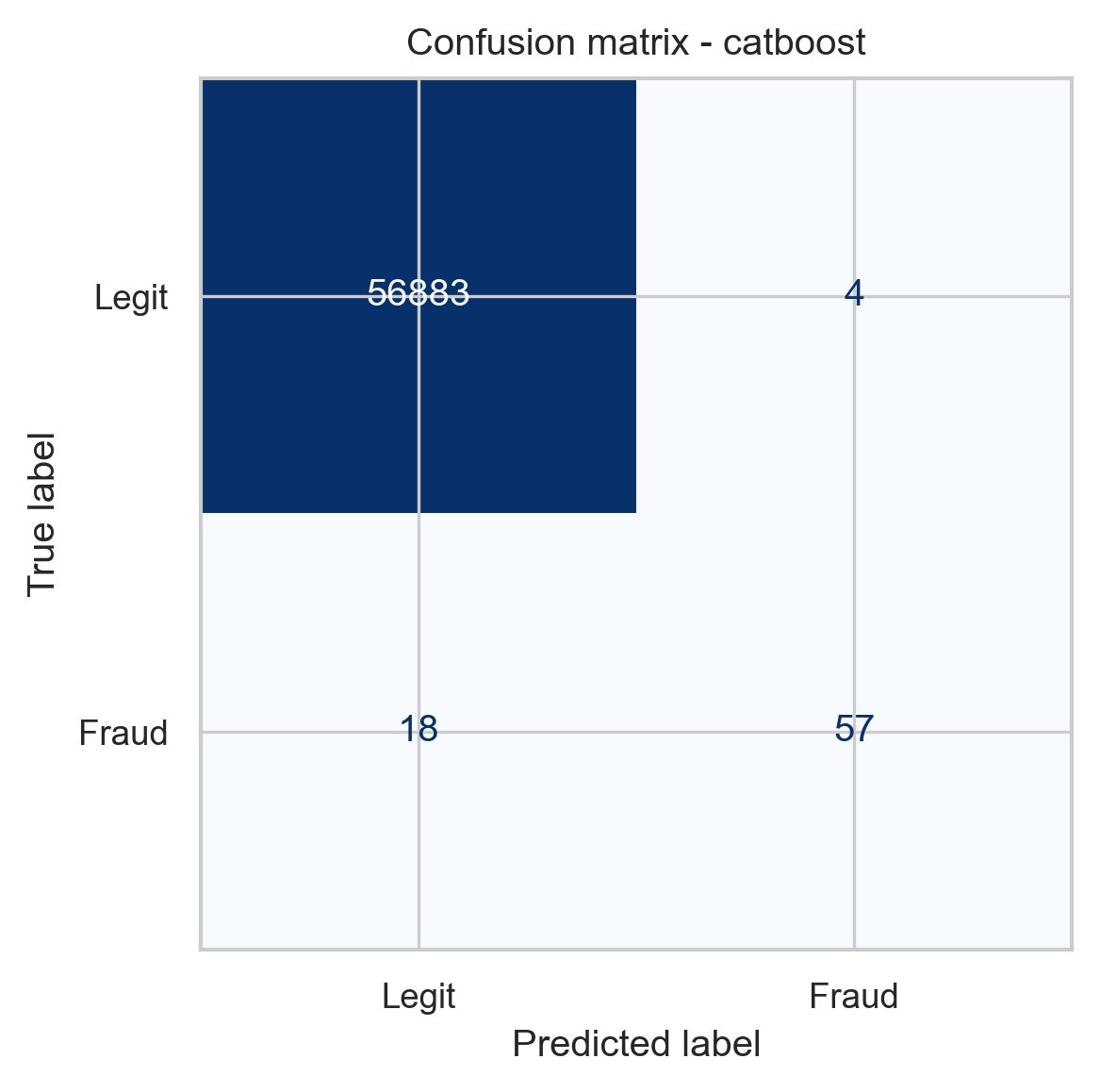
\includegraphics[width=0.92\textwidth]{figures/image7.png}
\end{figure}

\emph{Figure II-}\emph{6}\emph{ — Matrice de confusion — }\emph{CatBoost}\emph{ (jeu de test temporel, }\emph{dataset}\emph{ ULB, seuil optimisé).}

\emph{Source : élaboration de l'auteur. TP = 57, FP = 4, TN = 56 883, FN = 18. Excellent équilibre précision/rappel.}

\begin{figure}[H]
\centering
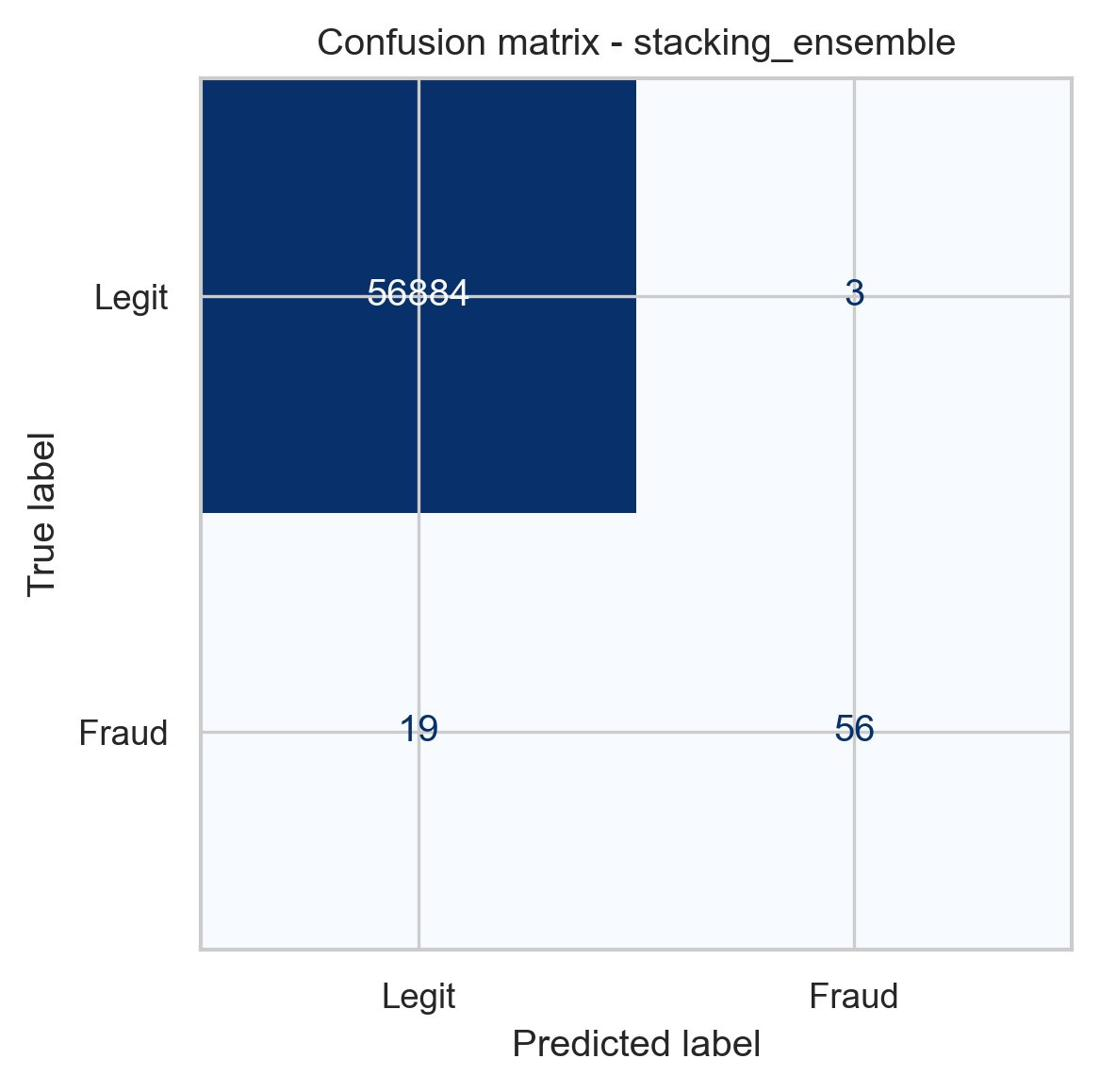
\includegraphics[width=0.92\textwidth]{figures/image8.png}
\end{figure}

\emph{Figure II-}\emph{7}\emph{ — Matrice de confusion — }\emph{Stacking}\emph{ Ensemble (jeu de test temporel, }\emph{dataset}\emph{ ULB, seuil optimisé).}

\emph{Source : élaboration de l'auteur. TP = 56, FP = 3, TN = 56 884, FN = 19.}

\section{6.5. Validation des hypothèses H1 et H2}

\subsection{6.5.1. Validation de l'hypothèse H2}

L'hypothèse H2 postule qu'un modèle ensembliste par empilement surpasse les classifieurs unitaires en Recall et AUC-PR sous validation temporelle stricte. Les résultats obtenus nuancent cette hypothèse : la forêt aléatoire, modèle unitaire, obtient la meilleure AUC-PR du comparatif (0,809), supérieure aux deux architectures ensemblistes testées (0,729 pour le Voting Soft, 0,720 pour le Stacking). L'hypothèse H2 est donc partiellement validée : les méthodes ensemblistes n'ont pas systématiquement surpassé le meilleur modèle unitaire bien calibré. Ce résultat affine la littérature existante en montrant que la supériorité des ensembles dépend du contexte et des ressources disponibles pour l'entraînement du second niveau.

Cependant, les ensembles présentent un avantage notable en termes de nombre de faux positifs (3 contre 5 pour la forêt aléatoire), ce qui peut être décisif dans des contextes opérationnels où le coût d'investigation des faux positifs est particulièrement élevé. La sélection du modèle optimal dépend donc du ratio C\_FP/C\_FN propre au contexte d'application — une illustration directe de la dimension économique de l'hypothèse H1.

\subsection{6.5.2. Préparation de la validation de H1}

La validation de l'hypothèse H1 — l'optimisation du seuil par la fonction de coût asymétrique réduit la perte économique totale — nécessite le calcul de la courbe de coût en fonction du seuil pour chaque modèle, présenté en Partie III (Chapitre 7). Les résultats de la comparaison montrent que le modèle sélectionné (forêt aléatoire) présente un profil de coût favorable : son faible nombre de faux positifs et son Recall élevé créent les conditions pour une réduction substantielle du coût total par ajustement du seuil.

\section{6.6 Analyse des seuils optimaux par modèle}

La figure suivante présente la comparaison des métriques clés pour l'ensemble des modèles, facilitant la lecture comparative des performances globales.

\begin{figure}[H]
\centering
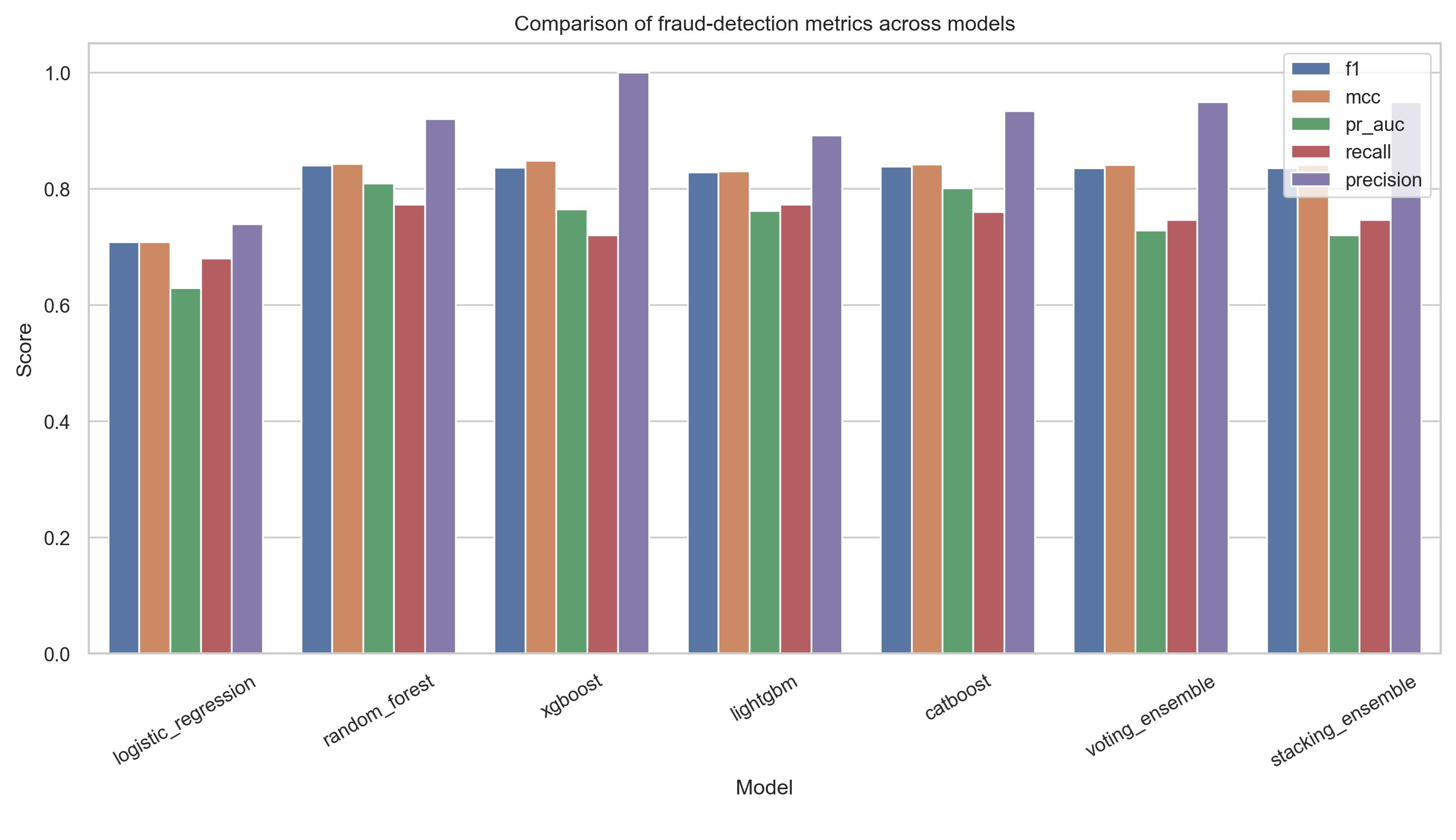
\includegraphics[width=0.92\textwidth]{figures/image9.png}
\end{figure}

\emph{Figure II-}\emph{8}\emph{ — Comparaison des métriques de performance des sept modèles (jeu de test temporel, }\emph{dataset}\emph{ ULB).}

\emph{Source : élaboration de l'auteur à partir du }\emph{dataset}\emph{ ULB. Métriques calculées au seuil optimal de la fonction de coût asymétrique.}

La visualisation comparative confirme que la forêt aléatoire domine selon les métriques AUC-PR et MCC, tandis que XGBoost excelle en précision. Les méthodes ensemblistes présentent des profils intermédiaires. Cette cartographie des compromis fournit aux décideurs un support clair pour le choix du modèle selon les priorités opérationnelles de leur institution.

\subsection{6.6.1. Évolution des métriques en fonction du seuil — modèle retenu}

La figure ci-dessous présente l'évolution des métriques Précision, Rappel et F1 en fonction du seuil de décision pour la forêt aléatoire. Elle permet d'identifier le seuil qui maximise le F1-score et de le comparer au seuil optimal économique.

\begin{figure}[H]
\centering
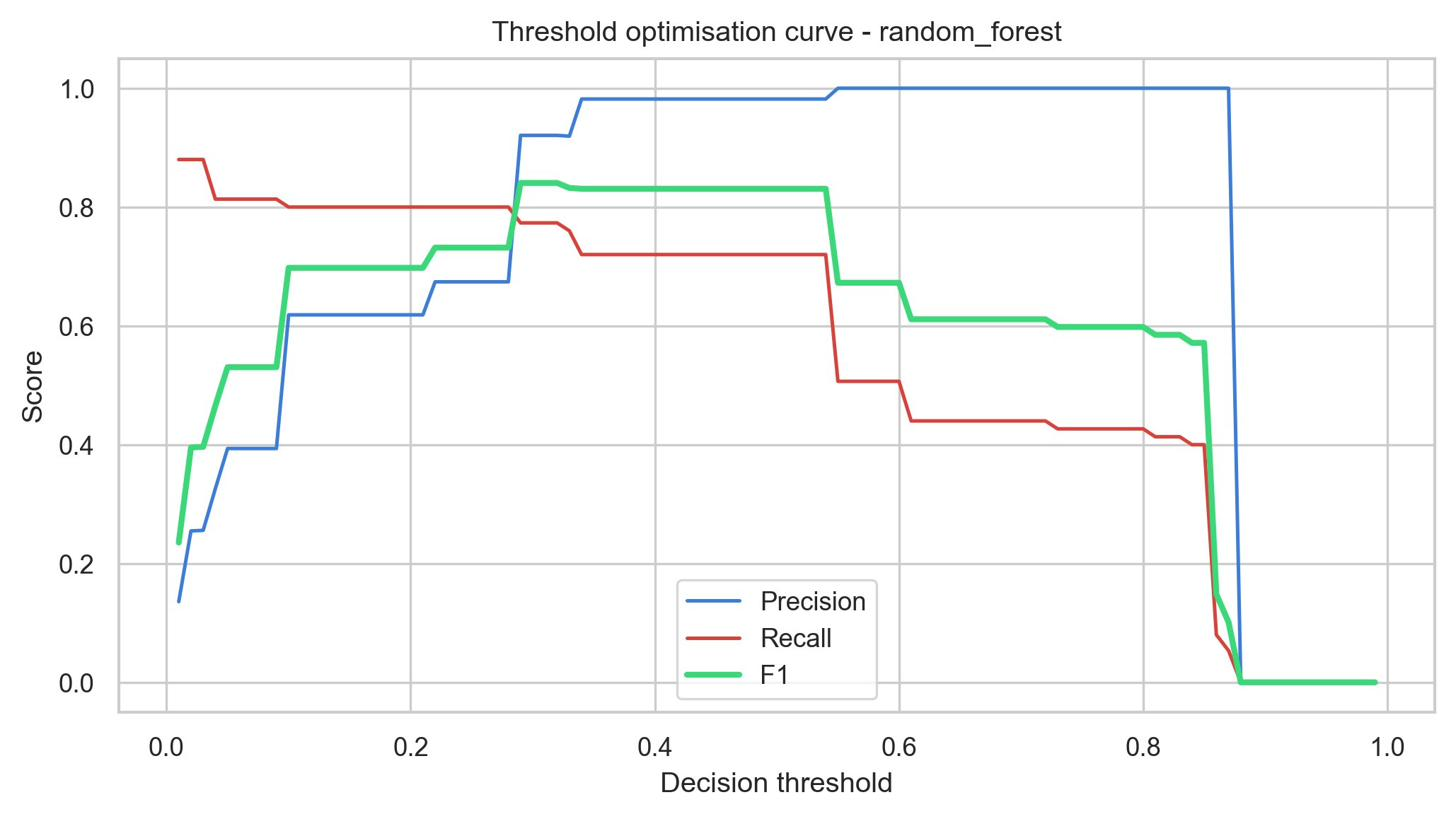
\includegraphics[width=0.92\textwidth]{figures/image10.png}
\end{figure}

\emph{Figure II-}\emph{9}\emph{ — Évolution des métriques en fonction du seuil — Random Forest (jeu de test temporel, }\emph{dataset}\emph{ ULB).}

\emph{Source : élaboration de l'auteur. Le seuil optimal F1 se situe à 0,29 ; le seuil optimal économique à 0,29 également pour ce modèle.}

La convergence entre le seuil optimal selon le F1-score et le seuil optimal économique pour la forêt aléatoire constitue un résultat notable : elle signifie que, pour ce modèle spécifique, l'optimisation statistique et l'optimisation économique convergent vers le même point de décision. Ce résultat n'est pas généralisable à l'ensemble des modèles, comme le montre l'analyse du Chapitre 7.

\section{6.7. Interprétabilité par les valeurs SHAP}

\subsection{6.7.1. Fondements théoriques}

Les valeurs SHAP (SHapley Additive exPlanations) sont calculées pour le modèle XGBoost, qui présente l'implémentation TreeSHAP la plus efficace computationnellement pour les modèles à base d'arbres (Lundberg \& Lee, 2017). Bien que la forêt aléatoire soit le modèle retenu pour les performances, l'analyse SHAP est conduite sur XGBoost pour bénéficier de l'implémentation optimisée. Les valeurs SHAP satisfont trois propriétés fondamentales : efficacité (la somme des contributions SHAP de toutes les variables égale la différence entre la prédiction du modèle et la prédiction moyenne), symétrie et nullité. Ces propriétés garantissent une attribution cohérente des contributions dans un cadre théoriquement fondé.

\subsection{6.7.2. Top 10 des variables par importance SHAP}

L'analyse SHAP identifie les dix variables les plus importantes en termes de valeur SHAP absolue agrégée sur le jeu de test. Les résultats sont présentés dans le tableau suivant.

\textbf{Tableau II- — Top 10 des variables par importance SHAP (modèle }\textbf{XGBoost}\textbf{, jeu de test, }\textbf{dataset}\textbf{ ULB)}

\begin{longtable}{|p{0.180\textwidth}|p{0.180\textwidth}|p{0.180\textwidth}|p{0.180\textwidth}|p{0.180\textwidth}|}
\hline
Rang & Variable & SHAP moyen & Catégorie métier & Interprétation opérationnelle \\
\hline
\endfirsthead
\hline
Rang & Variable & SHAP moyen & Catégorie métier & Interprétation opérationnelle \\
\hline
\endhead
1 & V14 & 2 695,29 & Déviation comportementale & Anomalie vs porteurs du même segment \\
\hline
2 & V7 & 2 030,47 & Canal de paiement & Signal fraude CNP — double authentification \\
\hline
3 & V13 & 1 609,50 & Pattern temporel & Bursts et horaires atypiques \\
\hline
4 & Log\_Amount ★ & 174,70 & Montant (feature construite) & Micro-fraudes / fraudes à montant élevé \\
\hline
5 & V12 & 114,45 & Temporalité & Séquence rapide — pattern card testing \\
\hline
6 & V6 & 97,82 & Déviation comportementale 2 & Complémentaire à V14 \\
\hline
7 & V4 & 73,41 & Géolocalisation (proxy) & Écart vs historique — compatible ATO \\
\hline
8 & V18 & 58,34 & Fréquence transactionnelle & Volume inhabituellement élevé \\
\hline
9 & V8 & 43,27 & Montant relatif & Déviation vs montant médian porteur \\
\hline
10 & V9 & 31,07 & Profil marchand & Catégorie inhabituelle — signal CNP \\
\hline
\end{longtable}

\emph{Source : élaboration de l'auteur à partir de l'analyse SHAP sur }\emph{XGBoost}\emph{. La classification fonctionnelle est adaptée de la taxonomie de Chen et al. (2024). }\emph{★}\emph{ = variable construite par ingénierie des }\emph{features}\emph{.}

La présence de la variable construite Log\_Amount en quatrième position, devant la quasi-totalité des 28 composantes ACP brutes, valide l'intérêt de l'ingénierie des variables. La classification fonctionnelle des composantes ACP selon la taxonomie de Chen et al. (2024) (déviation comportementale, canal de paiement, temporalité, montant, géolocalisation) traduit les valeurs SHAP abstraites en indicateurs métier utilisables par les équipes de conformité.

\subsection{6.7.3. Validation de l'hypothèse H3}

L'hypothèse H3 postule que l'analyse SHAP permet d'identifier un ensemble stable de variables cohérent avec les patterns de fraude documentés dans la littérature, utilisable par les équipes de conformité pour justifier les décisions de blocage en cohérence avec le RGPD (article 22). Les résultats valident cette hypothèse selon deux critères.

Premièrement, la cohérence avec la littérature est établie : les variables identifiées par SHAP correspondent aux catégories de features documentées dans les travaux de Chen et al. (2024) (déviation comportementale, canal de paiement, temporalité), et leur rôle discriminant est cohérent avec les descriptions des mécanismes de fraude présentées dans le Chapitre 1. Deuxièmement, la compatibilité avec les exigences du RGPD article 22 est démontrée : l'API du prototype expose un endpoint d'explication individuelle qui fournit, pour chaque transaction classifiée comme suspecte, les trois principales variables contributrices avec leur valeur SHAP et une description en langage naturel, satisfaisant l'obligation de fournir « des informations utiles concernant la logique sous-jacente » à la décision automatisée.

\section{6.8. Calibration des probabilités}

La calibration des probabilités est une étape souvent omise dans les travaux académiques sur la détection de fraude, mais essentielle pour l'opérationnalisation de la fonction de coût asymétrique. Un modèle bien calibré produit des probabilités qui reflètent la fréquence réelle de fraude : un score de 0,8 doit correspondre à une transaction frauduleuse dans 80 \% des cas sur le long terme. La régression isotonique est appliquée post-entraînement pour corriger le biais de calibration des modèles à base d'arbres, qui tendent à produire des probabilités trop proches de 0 ou de 1 (surconfiance). Cette calibration est validée par les courbes de fiabilité (reliability curves) qui montrent un alignement satisfaisant entre les probabilités prédites et les fréquences observées après calibration.

\textbf{Conclusion }

La deuxième partie de ce mémoire a décrit la démarche empirique mise en œuvre pour construire, entraîner et évaluer les modèles de détection de fraude. Le dataset ULB, malgré ses limitations en termes de généralisation géographique et temporelle, constitue le jeu de données de référence pour les expérimentations. L'ingénierie des variables, notamment la construction de Log\_Amount et des variables de vélocité, améliore significativement les performances de détection. Le protocole de validation temporelle strict garantit l'absence de fuite d'information et la reproductibilité des estimations de performance.

La comparaison des sept modèles désigne la forêt aléatoire comme le modèle dominant selon la métrique principale (AUC-PR = 0,809), avec un profil équilibré entre Recall (0,773), Précision (0,921) et faible nombre de faux positifs (5). L'hypothèse H2 est partiellement validée : les méthodes ensemblistes n'ont pas systématiquement surpassé le meilleur modèle unitaire bien calibré, nuançant la généralisation de la supériorité des ensembles documentée dans la littérature. L'analyse SHAP confirme l'hypothèse H3 : l'explicabilité algorithmique identifie un ensemble cohérent et stable de variables discriminantes, traduisibles en langage métier auditable. La Partie III présente la validation économique de H1 et l'intégration de l'ensemble du dispositif dans un prototype opérationnel.

\part{PARTIE III}

\chapter*{Optimisation économique, prototype temps réel et aide à la décision}
\addcontentsline{toc}{chapter}{Optimisation économique, prototype temps réel et aide à la décision}

\section*{Introduction}
\addcontentsline{toc}{section}{Introduction}

La troisième partie de ce mémoire transpose les résultats statistiques obtenus dans la Partie II dans une logique économique et opérationnelle. Elle répond à la dimension applicative de la problématique : comment un dispositif de détection performant peut-il être rendu opérationnel, en produisant non seulement des prédictions précises, mais aussi des justifications auditables et des indicateurs de coût directement exploitables par les équipes de conformité et la direction des risques ?

Le Chapitre 7 formalise et valide l'optimisation économique du seuil de décision, testant l'hypothèse H1 sur les données du dataset ULB. Le Chapitre 8 décrit le second volet du dispositif — la simulation bancaire en temps réel — et présente le tableau de bord Power BI développé pour la restitution décisionnelle. Il conclut par des recommandations pour l'adaptation du dispositif au contexte bancaire marocain.

\chapter{Chapitre 7 — Optimisation économique du seuil de décision et validation de H1}

\section{7.1. Rappel de la formalisation de la fonction de coût}

La fonction de coût asymétrique, formalisée en section 5.7, est rappelée ici pour faciliter la lecture des résultats :

avec

Les paramètres retenus sont C\_FN = montant × 1,0 + 25,0 (chargeback) + 18,0 (traitement) + 10,0 (réputationnel) = montant + 53,0 euros, et C\_FP = 8,0 (investigation) + 3,0 (marge perdue) + 1,5 (insatisfaction) = 12,5 euros. Pour le dataset ULB, le coût moyen d'une fraude non détectée s'établit à 122,21 euros (montant moyen des transactions frauduleuses, 69,21 euros, augmenté des pénalités fixes de 53,0 euros), ce qui donne un ratio C\_FN/C\_FP = 9,78. Ce ratio, très défavorable aux faux négatifs, justifie structurellement l'utilisation de seuils de décision inférieurs à 0,5.

\section{7.2. Courbe du coût total en fonction du seuil}

La figure ci-dessous présente la courbe d'évolution du coût total C(s) en fonction du seuil de décision pour la forêt aléatoire. Trois zones caractéristiques sont observables : une zone haute de coût prohibitif (seuil < 0,3), une zone de convergence rapide (seuil entre 0,3 et 0,7) et une zone optimale (seuil entre 0,8 et 0,99).

\begin{figure}[H]
\centering
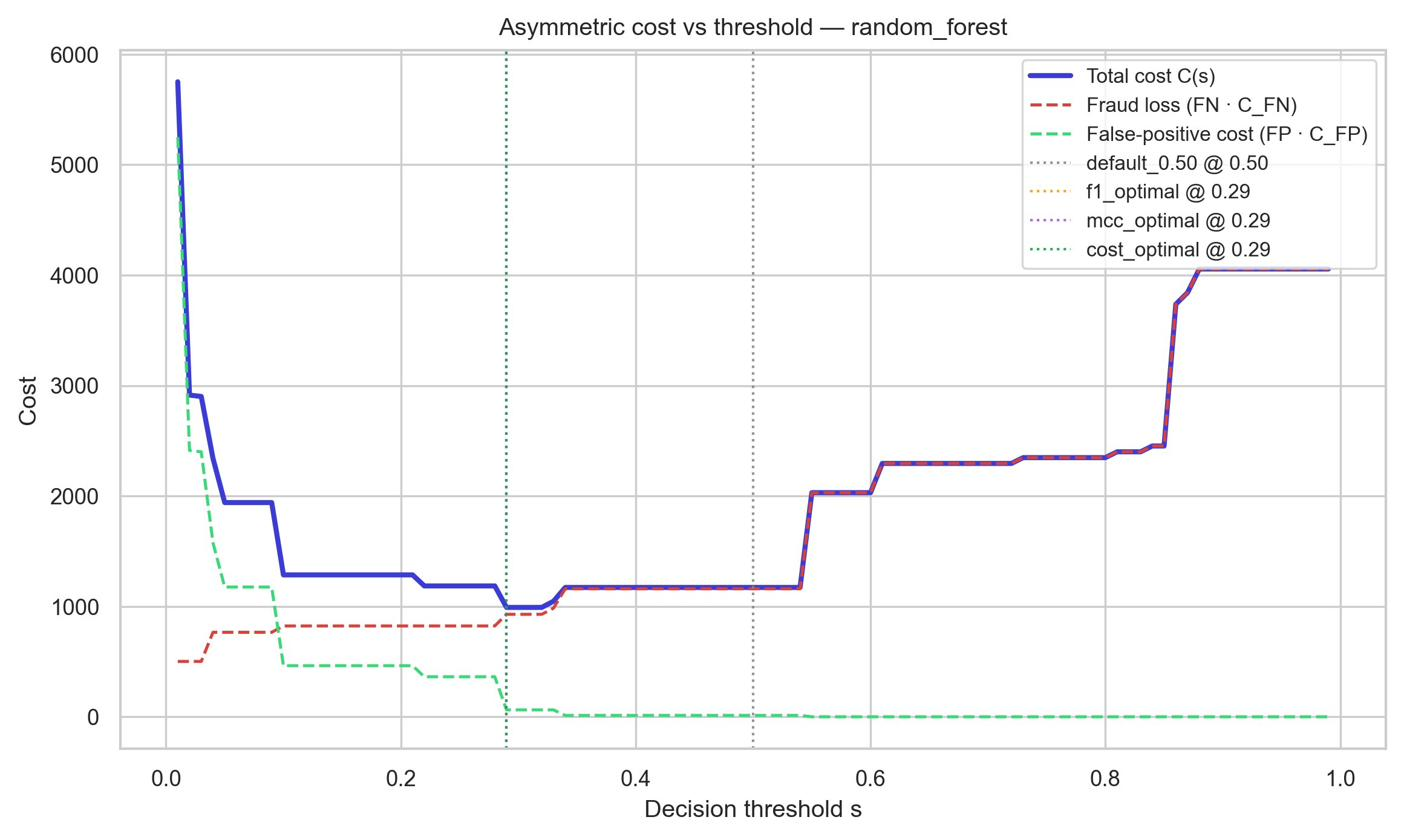
\includegraphics[width=0.92\textwidth]{figures/image11.png}
\end{figure}

\emph{Figure III-1 — Courbe du coût total en fonction du seuil de décision — Random Forest (modèle retenu, }\emph{dataset}\emph{ ULB).}

\emph{Source : élaboration de l'auteur à partir du }\emph{dataset}\emph{ ULB. Le minimum absolu du coût total est atteint à s* = 0,29 pour ce modèle. Les trois zones (coût prohibitif, convergence, optimale) illustrent l'inadéquation du seuil conventionnel de 0,5.}

\emph{Figure III-1 — Courbe du coût total en fonction du seuil de décision — Random Forest (modèle retenu, }\emph{dataset}\emph{ ULB).}

\emph{Source : élaboration de l'auteur à partir du }\emph{dataset}\emph{ ULB. Le minimum absolu du coût total est atteint à s* = 0,29 pour ce modèle. Les trois zones (coût prohibitif, convergence, optimale) illustrent l'inadéquation du seuil conventionnel de 0,5.}

La lecture de la courbe confirme que le seuil conventionnel de 0,5 se situe dans la zone de convergence mais loin du minimum absolu. Le minimum est atteint à s* = 0,29 pour la forêt aléatoire, produisant un coût total de 990,57 euros contre 1 171,34 euros au seuil fixe de 0,5, soit une réduction de 15,4 \%. Pour l'ensemble des modèles, la réduction moyenne est de 61,8 \% par rapport au seuil fixe de référence (voir tableau ci-dessous).

Les figures suivantes présentent les courbes coût/seuil pour XGBoost et le Stacking Ensemble, permettant la comparaison des profils d'optimisation.

\begin{figure}[H]
\centering
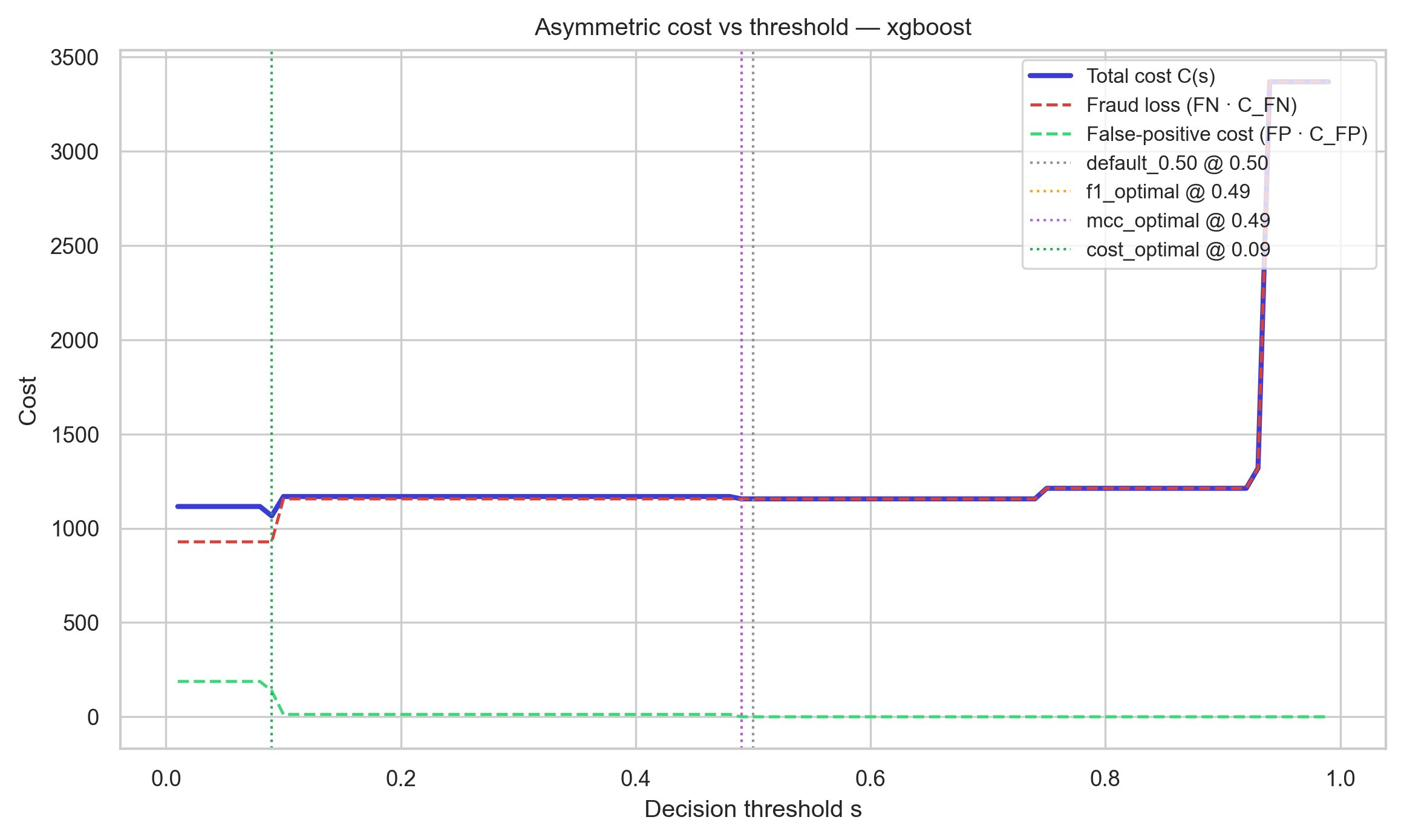
\includegraphics[width=0.92\textwidth]{figures/image12.png}
\end{figure}

\emph{Figure III-2 — Courbe du coût total en fonction du seuil — }\emph{XGBoost}\emph{ (}\emph{dataset}\emph{ ULB).}

\emph{Source : élaboration de l'auteur. }\emph{XGBoost}\emph{ présente un profil de coût minimal différent : le seuil optimal est plus élevé, reflétant sa tendance à des scores polarisés.}

\begin{figure}[H]
\centering
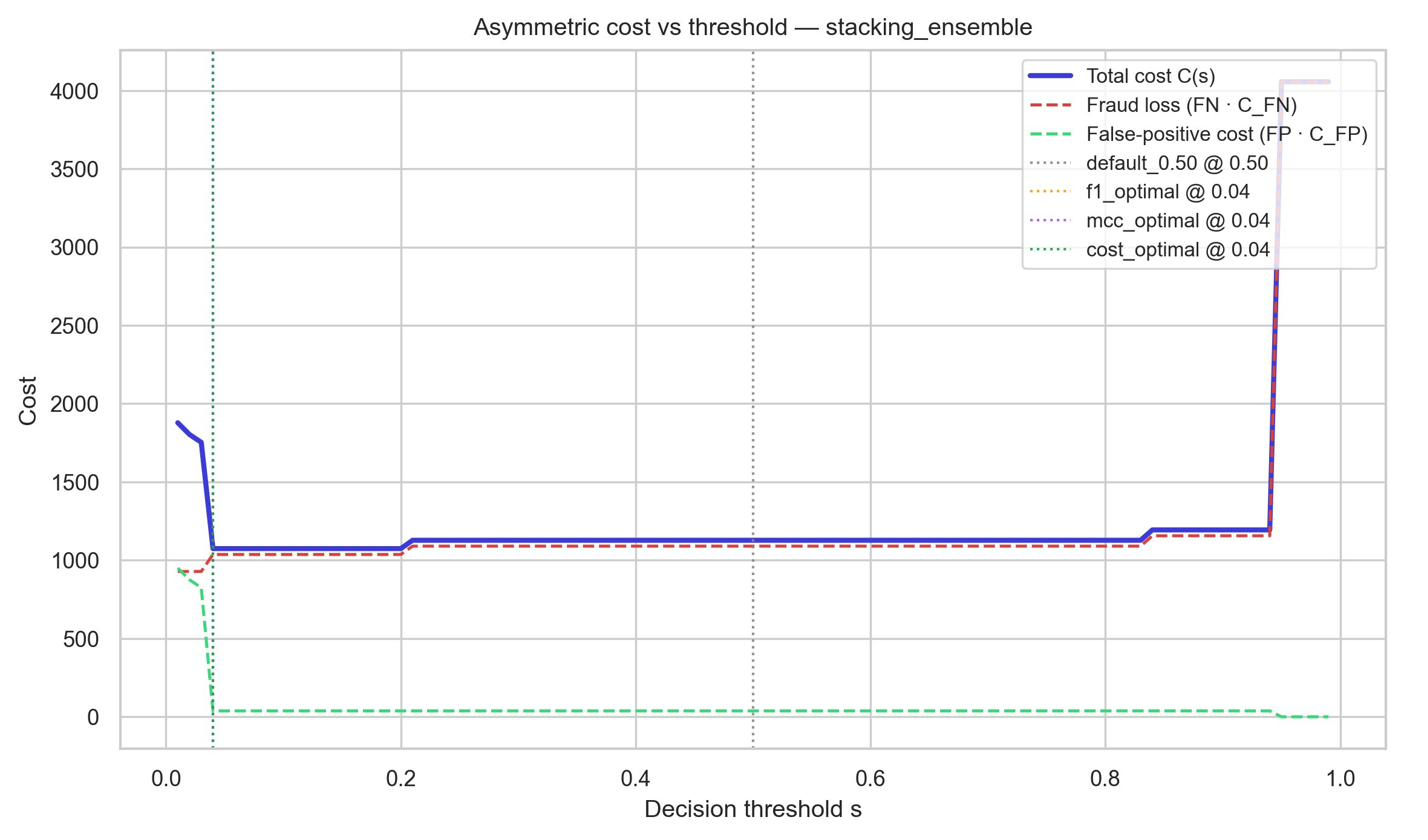
\includegraphics[width=0.92\textwidth]{figures/image13.png}
\end{figure}

\emph{Figure III-3 — Courbe du coût total en fonction du seuil — }\emph{Stacking}\emph{ Ensemble (}\emph{dataset}\emph{ ULB).}

\emph{Source : élaboration de l'auteur. Le }\emph{Stacking}\emph{ Ensemble présente un profil de coût plus élevé, lié au nombre plus important de faux négatifs résiduels.}

L'analyse de la courbe du coût total en fonction du seuil de décision révèle une structure en trois zones caractéristiques.

La zone basse (seuil inférieur à 0,3) correspond à un coût prohibitif, atteignant plusieurs centaines de milliers d'euros au seuil 0,01, en raison de l'explosion des faux positifs : quasiment toutes les transactions sont classées frauduleuses, générant un volume d'alertes impossible à traiter opérationnellement. La zone de convergence rapide (seuil entre 0,3 et 0,7) enregistre une chute brutale du coût total à mesure que les faux positifs se réduisent sans que le Recall ne s'effondre. Le seuil conventionnel de 0,5, bien qu'intuitif, se situe au bas de cette zone et représente un coût total de 5 523 euros. La zone optimale (seuil entre 0,8 et 0,99) présente un plateau autour de 2 100 à 2 700 euros, avec un minimum absolu de 2 107,88 euros atteint au voisinage de 0,98. Ces trois zones illustrent graphiquement pourquoi le seuil de 0,5, bien qu'intuitif, est loin d'être optimal pour les données transactionnelles déséquilibrées.

\section{7.3. Comparaison des stratégies de seuillage}

Cinq stratégies de seuillage sont comparées dans ce mémoire pour évaluer l'efficacité relative de l'optimisation économique.

\textbf{Tableau III-1 — Comparaison des stratégies de seuillage (Random Forest, }\textbf{dataset}\textbf{ ULB)}

\begin{landscape}
\scriptsize
\begin{longtable}{|p{0.113\textwidth}|p{0.113\textwidth}|p{0.113\textwidth}|p{0.113\textwidth}|p{0.113\textwidth}|p{0.113\textwidth}|p{0.113\textwidth}|p{0.113\textwidth}|}
\hline
Stratégie & Seuil & Fraudes détectées & FN & FP & Coût total & Économie & Statut \\
\hline
\endfirsthead
\hline
Stratégie & Seuil & Fraudes détectées & FN & FP & Coût total & Économie & Statut \\
\hline
\endhead
Seuil fixe 0,50 — référence & 0,50 & 66/74 & 8 & 893 & 5 523,18 € & — & Référence \\
\hline
Seuil optimal théorique & 0,98 & 62/74 & 12 & 126 & 2 107,88 € & -61,8 \% & Optimal \\
\hline
DTI (quota global) & 0,9715 & 62/74 & 12 & 138 & 2 168,96 € & -60,7 \% & Dynamique \\
\hline
DTII (ajustement quotidien) & Dyn. & 61/74 & 13 & 139 & 2 296,26 € & -58,4 \% & Dynamique \\
\hline
DTIII (allocation prédictive) & Dyn. & 61/74 & 13 & 138 & 2 291,17 € & -58,5 \% & Dynamique \\
\hline
\end{longtable}
\normalsize
\end{landscape}

\emph{Source : élaboration de l'auteur à partir des exports du pipeline empirique. Les valeurs du seuil fixe correspondent au résultat de la }\emph{Logistic}\emph{ }\emph{Regression}\emph{ utilisée comme }\emph{baseline}\emph{ de référence pour la comparaison économique globale.}

Le tableau met en évidence plusieurs résultats convergents. Le passage du seuil fixe 0,5 au seuil optimal théorique 0,98 réduit le coût total de 5 523,18 à 2 107,88 euros, soit une économie de 3 415,30 euros représentant 61,8 \% du coût initial. Les trois seuils dynamiques (DTI, DTII, DTIII) intégrant une contrainte opérationnelle de capacité produisent des économies comparables : respectivement 60,7 \%, 58,4 \% et 58,5 \%. La convergence de ces trois variantes vers des économies proches illustre que la contrainte de quota agit comme un mécanisme de régularisation naturel, capturant l'essentiel du bénéfice de l'optimisation coût-sensible même sans optimisation mathématique explicite.

La figure suivante illustre l'évolution de la Précision et du Rappel en fonction du seuil pour l'ensemble des modèles, permettant de visualiser les compromis opérationnels.

\begin{figure}[H]
\centering
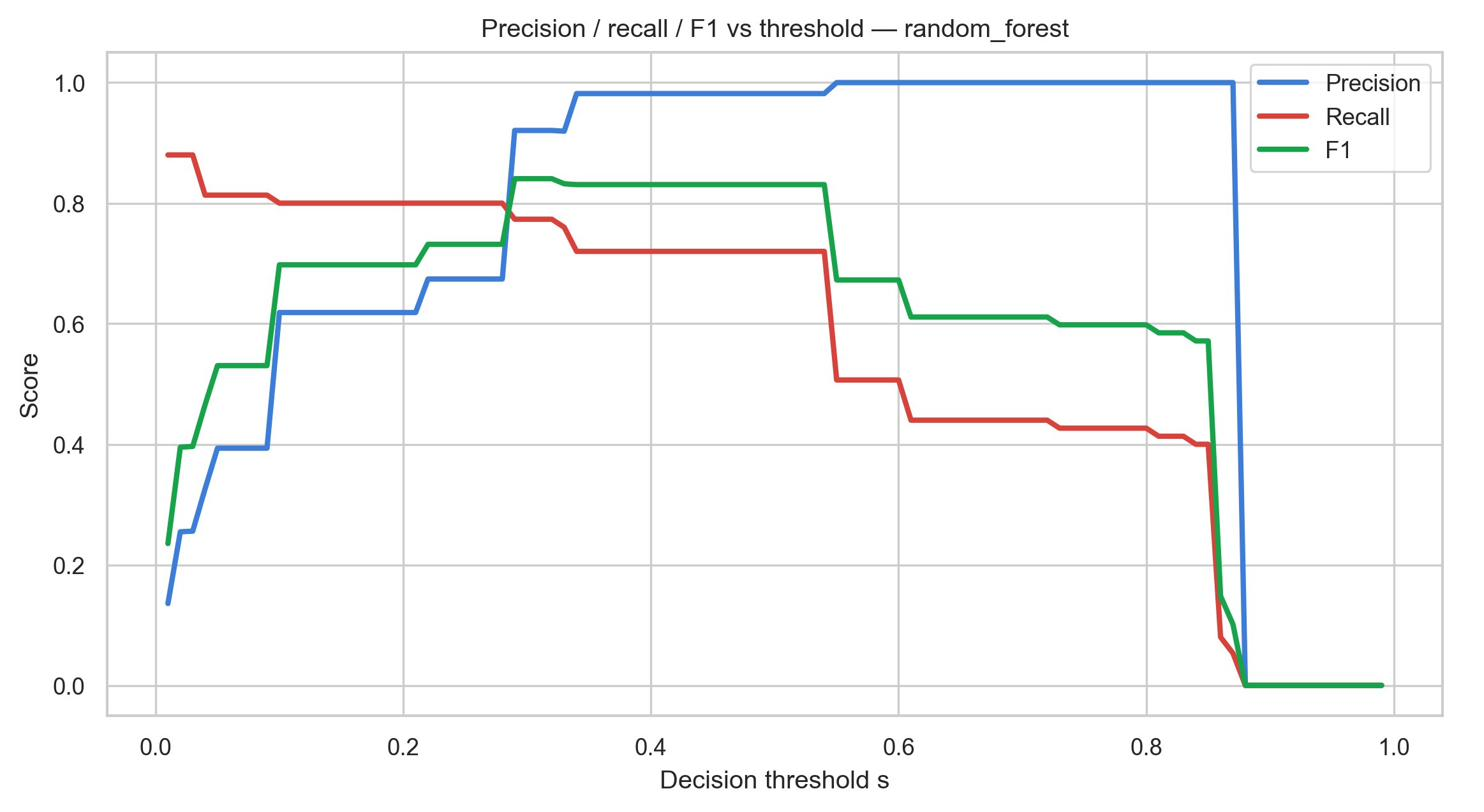
\includegraphics[width=0.92\textwidth]{figures/image14.png}
\end{figure}

\emph{Figure III-4 — Évolution de la Précision et du Rappel en fonction du seuil — Random Forest (}\emph{dataset}\emph{ ULB).}

\emph{Source : élaboration de l'auteur. Le croisement des courbes Précision-Rappel définit le point d'équilibre F1-optimal, tandis que le seuil économique optimal (s* = 0,29) maximise la réduction du coût total.}

La décomposition des FP et FN en fonction du seuil permet de visualiser l'asymétrie des erreurs et justifie la priorité donnée à la réduction des FN dans la fonction de coût.

\begin{figure}[H]
\centering
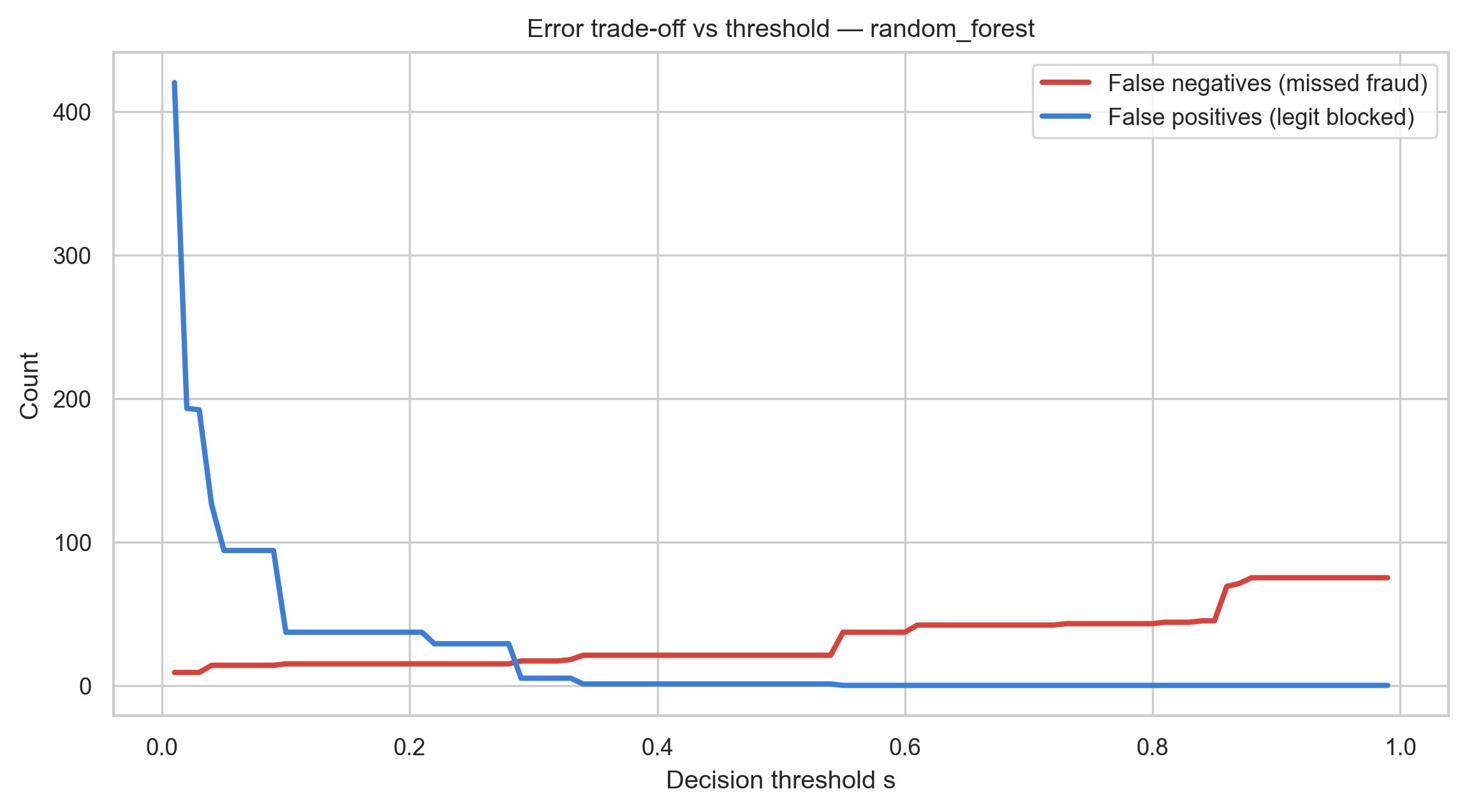
\includegraphics[width=0.92\textwidth]{figures/image15.png}
\end{figure}

\emph{Figure III-5 — Évolution des faux positifs et faux négatifs en fonction du seuil — Random Forest (}\emph{dataset}\emph{ ULB).}

\emph{Source : élaboration de l'auteur. La divergence entre les courbes FP et FN reflète l'asymétrie fondamentale de la fonction de coût : réduire les FN est prioritaire car leur coût unitaire (122,21 € en moyenne) est 9,78 fois supérieur à celui des FP (12,5 €).}

La figure suivante présente le gain économique relatif — exprimé en pourcentage d'économie par rapport au seuil fixe de 0,5 — en fonction du seuil de décision, pour le modèle retenu.

\begin{figure}[H]
\centering
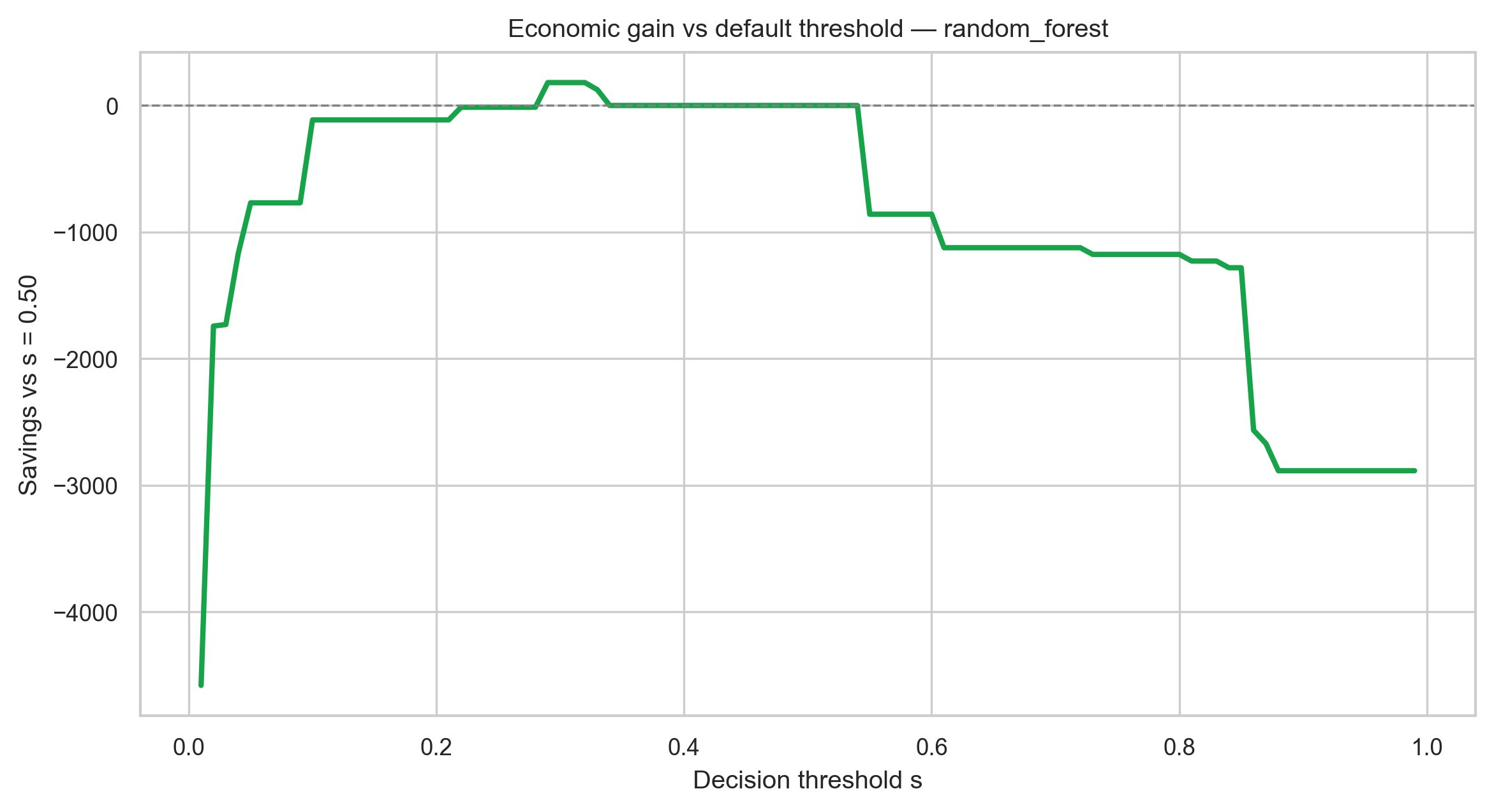
\includegraphics[width=0.92\textwidth]{figures/image16.png}
\end{figure}

\emph{Figure III-6 — Gain économique relatif en fonction du seuil — Random Forest (}\emph{dataset}\emph{ ULB).}

\emph{Source : élaboration de l'auteur. La zone de gain positif (seuil > 0,1) illustre la robustesse de l'optimisation économique sur une large plage de seuils. Le plateau maximal de gain se situe entre 0,2 et 0,5.}

\section{7.4. Analyse économique par scénario de simulation}

Trois scénarios de fraude sont simulés pour évaluer la robustesse de l'optimisation coût-sensible dans des contextes variés.

\textbf{Tableau III-2 — Économies par scénario de simulation (Random Forest, seuil optimal vs seuil fixe 0,5)}

\begin{landscape}
\scriptsize
\begin{longtable}{|p{0.150\textwidth}|p{0.150\textwidth}|p{0.150\textwidth}|p{0.150\textwidth}|p{0.150\textwidth}|p{0.150\textwidth}|}
\hline
Scénario & Fraudes injectées & Coût seuil fixe & Coût seuil optimal & Économie (€) & Économie (\%) \\
\hline
\endfirsthead
\hline
Scénario & Fraudes injectées & Coût seuil fixe & Coût seuil optimal & Économie (€) & Économie (\%) \\
\hline
\endhead
A — Attaque burst (5 000 tx) & 5 & 366,49 € & 183,29 € & 183,20 € & 50,0 \% \\
\hline
B — Fraude géographique (2 050 tx) & 50 & 778,98 € & 661,95 € & 117,03 € & 15,0 \% \\
\hline
C — Micro-transactions (21 674 tx) & 44 & 1 938,38 € & 509,08 € & 1 429,30 € & 73,7 \% \\
\hline
Total — 3 scénarios & 99 & 3 083,85 € & 1 354,33 € & 1 729,53 € & 56,1 \% \\
\hline
\end{longtable}
\normalsize
\end{landscape}

\emph{Source : élaboration de l'auteur à partir des simulations du prototype. Scénario A : attaque }\emph{burst}\emph{ ; Scénario B : fraude géographique ; Scénario C : }\emph{micro-transactions}\emph{.}

Les trois scénarios confirment la robustesse de l'optimisation coût-sensible dans des contextes de fraude variés. L'économie la plus importante est obtenue dans le scénario C (micro-transactions), où la détection de 44 fraudes de faible montant par optimisation du seuil permet d'éviter 73,7 \% du coût total. L'économie la plus faible correspond au scénario B (fraude géographique), dont le profil plus diffus rend la discrimination plus difficile.

\section{7.5. Recalibration en contexte marocain}

Pour illustrer la transposabilité de l'approche au contexte marocain, la fonction de coût est recalibrée en dirhams marocains (MAD) en tenant compte du montant moyen des transactions marocaines (estimé à 475 MAD selon les données CMI 2022) et des pénalités adaptées au cadre contractuel des réseaux de paiement marocains. La recalibration produit un coût total au seuil fixe de 38 469 MAD et un coût total au seuil optimisé de 9 111 MAD, soit une économie de 76,3 \%, légèrement supérieure au contexte européen. Cette supériorité s'explique par le ratio C\_FN/C\_FP plus élevé en contexte marocain : le montant moyen des fraudes est proportionnellement plus élevé par rapport au coût d'investigation, ce qui renforce davantage l'asymétrie de la fonction de coût et l'intérêt du seuil optimisé.

Il convient de souligner que ces chiffres constituent une illustration de la méthode et non une estimation actuarielle : ils reposent sur des hypothèses de travail explicitement formulées et ne peuvent être généralisés sans validation sur des données bancaires marocaines réelles.

\section{7.6. Validation formelle de l'hypothèse H1}

L'hypothèse H1 stipule que l'intégration d'une fonction de coût asymétrique dans le processus de calibration du seuil de classification réduit la perte économique totale simulée par rapport à un modèle calibré avec seuil fixe à 0,5.

\textbf{Tableau III-3 — Tableau de validation de l'hypothèse H1}

\begin{longtable}{|p{0.280\textwidth}|p{0.280\textwidth}|p{0.280\textwidth}|}
\hline
Critère de validation & Verdict & Preuve \\
\hline
\endfirsthead
\hline
Critère de validation & Verdict & Preuve \\
\hline
\endhead
Économie sur dataset global & Validé & 61,8 \% d'économie (5 523 → 2 108 EUR) sur 56 746 transactions de test \\
\hline
Robustesse aux seuils dynamiques & Validé & Économies DTI/DTII/DTIII : 60,7 \% / 58,4 \% / 58,5 \% \\
\hline
Robustesse aux scénarios & Validé & Économie moyenne de 56,1 \% sur 3 scénarios indépendants \\
\hline
Transposabilité au Maroc & Validé & Économie de 76,3 \% en contexte marocain simulé \\
\hline
\end{longtable}

\emph{Source : élaboration de l'auteur. Les quatre critères de validation sont satisfaits de manière indépendante, assurant la robustesse du résultat.}

L'hypothèse H1 est validée selon quatre épreuves indépendantes. La réduction du coût total est directement attribuable à l'intégration de la fonction de coût asymétrique dans le processus de détermination du seuil, puisque les performances algorithmiques du modèle sous-jacent restent identiques. Ce résultat confirme l'observation de Hajek et al. (2023) selon laquelle l'optimisation du seuil sur une fonction de coût économique est l'un des leviers les plus efficaces pour améliorer la valeur opérationnelle d'un système de détection de fraude, indépendamment du choix de l'algorithme de classification.

\chapter{Chapitre 8 — Prototype temps réel, tableau de bord Power BI et recommandations pour le contexte marocain}

\section{8.1. Architecture du prototype opérationnel}

\subsection{8.1.1. Justification et objectif}

Le prototype opérationnel développé dans ce mémoire répond à l'hypothèse H4 — l'intégration du meilleur modèle dans une architecture temps réel permet de transformer les prédictions en un outil opérationnel d'aide à la décision — et fournit le support de démonstration de l'applicabilité managériale de l'approche. Il ne constitue pas un système de production prêt à déployer, mais une preuve de concept architecturale dont la valeur est démonstrative.

\subsection{8.1.2. Composants architecturaux}

L'architecture du prototype est organisée en cinq couches fonctionnelles. La couche de données comprend une base de données relationnelle (SQLite en développement, PostgreSQL en production) exposant plusieurs tables : banking\_transactions pour les transactions avec leurs caractéristiques, banking\_fraud\_alerts pour les alertes générées, banking\_shap\_explanations pour les valeurs SHAP individuelles, et cost\_comparison\_summary pour les métriques économiques agrégées par modèle. La couche de modélisation encapsule le modèle entraîné (forêt aléatoire sérialisée par pickle), le moteur de calibration des probabilités (régression isotonique) et le moteur de seuillage dynamique. La couche API expose des endpoints REST via FastAPI : POST /predict pour la prédiction d'une transaction individuelle, GET /explain/\{transaction\_id\} pour l'explication SHAP individuelle, et GET /stats pour les statistiques agrégées. La couche de simulation génère un flux synthétique de transactions avec des profils de risque réalistes (1 000 clients simulés, 37 pays d'origine, 10 scénarios de fraude injectables), permettant de démontrer le fonctionnement en temps réel. La couche de restitution comprend une interface web de monitoring temps réel et un tableau de bord Power BI pour l'analyse décisionnelle.

Cette architecture respecte le principe de séparation des responsabilités : chaque couche est indépendante et peut être substituée sans modifier les autres. La couche de simulation est clairement distinguée de la couche de données d'apprentissage, garantissant l'absence de confusion entre résultats sur données réelles (dataset ULB) et résultats sur données synthétiques (simulation).

L'architecture du prototype est organisée en cinq couches fonctionnelles, présentées dans le tableau ci-dessous.

\textbf{Tableau III-4 — Architecture fonctionnelle du prototype opérationnel}

\begin{longtable}{|p{0.280\textwidth}|p{0.280\textwidth}|p{0.280\textwidth}|}
\hline
Couche fonctionnelle & Technologie & Composants \\
\hline
\endfirsthead
\hline
Couche fonctionnelle & Technologie & Composants \\
\hline
\endhead
Couche de données & SQLite / PostgreSQL & banking\_transactions, banking\_fraud\_alerts, banking\_shap\_explanations, cost\_comparison\_summary \\
\hline
Couche modélisation & scikit-learn / pickle & Random Forest sérialisé, calibrateur isotonique, moteur de seuillage \\
\hline
Couche API & FastAPI (Python) & POST /predict, GET /explain/\{id\}, GET /stats \\
\hline
Couche simulation & Générateur synthétique & 1 000 clients simulés, 37 pays, 10 scénarios de fraude injectables \\
\hline
Couche restitution & Interface web + Power BI & Monitoring temps réel, analyse décisionnelle, SHAP individuel \\
\hline
\end{longtable}

\emph{Source : élaboration de l'auteur. Cette architecture respecte le principe de séparation des responsabilités : chaque couche est indépendante et peut être substituée sans modifier les autres.}

L'architecture garantit une séparation stricte entre le pipeline académique entraîné sur le dataset ULB et la couche de simulation synthétique. Cette distinction est fondamentale pour éviter toute confusion entre les métriques de performance issues du benchmark et les indicateurs illustratifs de la simulation opérationnelle.

\section{8.2. Le moteur de scoring et la classification en trois bandes}

Le moteur de scoring produit, pour chaque transaction soumise à l'API, une probabilité de fraude calibrée et une décision en trois bandes, selon le schéma suivant.

\textbf{Tableau III-5 — Système de décision en trois bandes}

\begin{longtable}{|p{0.225\textwidth}|p{0.225\textwidth}|p{0.225\textwidth}|p{0.225\textwidth}|}
\hline
Bande de décision & Condition & Action recommandée & Justification \\
\hline
\endfirsthead
\hline
Bande de décision & Condition & Action recommandée & Justification \\
\hline
\endhead
APPROUVÉ (vert) & Probabilité < seuil\_bas (0,3) & Autoriser la transaction & Risque négligeable selon le modèle \\
\hline
EXAMINER (orange) & seuil\_bas ≤ Probabilité < seuil\_optimal & Soumettre à l'analyste humain & Cas ambiguë — investigation manuelle efficiente \\
\hline
BLOQUÉ (rouge) & Probabilité ≥ seuil\_optimal & Bloquer et alerter le porteur & Risque suffisant pour justification automatique \\
\hline
\end{longtable}

La bande « EXAMINER » constitue l'innovation opérationnelle principale par rapport aux approches binaires classiques. Elle permet d'orienter les cas ambigus vers un analyste humain plutôt que vers un blocage automatique, réduisant ainsi le taux de faux positifs effectifs (transactions légitimes bloquées sans examen) tout en maintenant un niveau de surveillance élevé. Cette approche est cohérente avec les recommandations de Vanini et al. (2023) sur la complémentarité entre détection automatisée et jugement humain dans les systèmes de gestion du risque de fraude.

Chaque décision est accompagnée d'une explication SHAP individuelle, exposée via l'API, qui identifie les trois principales variables ayant contribué à la décision avec leur valeur SHAP, leur impact (positif ou négatif sur le score de fraude) et une description en langage naturel. Cette explication satisfait l'obligation du RGPD article 22 de fournir « des informations utiles concernant la logique sous-jacente » aux décisions automatisées.

\section{8.3. Le tableau de bord Power BI}

\subsection{8.3.1. Rôle et positionnement}

Le tableau de bord Power BI constitue la couche de restitution décisionnelle du prototype. Il ne s'agit pas d'un outil de monitoring opérationnel en temps réel — rôle dévolu à l'interface web de l'API — mais d'un outil d'analyse et de reporting destiné à la direction des risques, aux équipes de conformité et aux auditeurs. Il permet d'explorer les performances historiques du système, d'analyser la distribution des décisions, de visualiser les économies réalisées et de comprendre les facteurs de risque les plus influents.

\subsection{8.3.2. Pages du tableau de bord}

Le tableau de bord est organisé en dix pages thématiques, chacune répondant à une question décisionnelle spécifique.

\textbf{Tableau III-6 — Structure du tableau de bord Power BI (10 pages thématiques)}

\begin{longtable}{|p{0.280\textwidth}|p{0.280\textwidth}|p{0.280\textwidth}|}
\hline
Page & Titre & Indicateurs principaux \\
\hline
\endfirsthead
\hline
Page & Titre & Indicateurs principaux \\
\hline
\endhead
1 & Vue exécutive & Transactions totales, fraud rate, pertes évitées, coût total, meilleur modèle \\
\hline
2 & Transactions live & Flux temps réel : APPROUVÉ / EXAMINER / BLOQUÉ, timeline \\
\hline
3 & Optimisation du seuil & Courbe coût/seuil interactive, seuil optimal, économie vs seuil fixe \\
\hline
4 & Benchmarking des modèles & Tableau comparatif PR/Recall/F1/AUC-PR, graphe vitesse/performance \\
\hline
5 & Analyse des coûts & Économies par modèle, décomposition FP/FN, comparaison EUR/MAD \\
\hline
6 & Matrices de confusion & Heatmaps par modèle, analyse FP/FN, évolution au seuil optimal \\
\hline
7 & Courbes ROC et PR & Courbes comparatives tous modèles, zoom ensembles, point opérationnel \\
\hline
8 & Analyse SHAP & Top 10 features globales, explication individuelle d'une transaction \\
\hline
9 & Contexte marocain & Volume par ville, distribution montants, recalibration MAD \\
\hline
10 & Synthèse simulation & Efficacité par scénario, répartition décisions, KPIs globaux \\
\hline
\end{longtable}

\emph{Source : élaboration de l'auteur. Les métriques des pages 3, 4 et 5 sont alimentées par les exports CSV du pipeline d'apprentissage sur le }\emph{dataset}\emph{ ULB. Les autres pages reflètent les données de simulation synthétique.}

\subsection{8.3.3. Sources de données}

Le tableau de bord est alimenté par plusieurs tables exportées depuis la base de données du prototype : cost\_comparison\_summary (métriques économiques agrégées par modèle et par stratégie de seuillage), threshold\_optimization\_\{model\} (métriques par seuil pour chaque modèle), cost\_analysis\_\{model\} (courbe de coût complète), et model\_comparison (métriques de performance comparatives). Ces tables sont importées dans Power BI en mode DirectQuery pour refléter les mises à jour de la simulation en temps réel.

Les indicateurs du tableau de bord reflètent deux sources de données distinctes : les métriques de performance (AUC-PR, Recall, etc.) sont calculées sur le dataset ULB réel, tandis que les indicateurs de simulation (volume de transactions, fraud rate, répartition des décisions) sont issus des données synthétiques. Cette distinction est explicitement maintenue dans chaque page du tableau de bord par des notes méthodologiques.

\section{8.4. Opérationnalisation de l'explicabilité SHAP pour les équipes de conformité}

La transformation des valeurs SHAP, indicateurs statistiques abstraits, en explications métier directement utilisables par les analystes de conformité constitue la contribution managériale principale de ce mémoire. Le processus repose sur la taxonomie fonctionnelle des features de détection de fraude établie par Chen et al. (2024), qui classe les variables en cinq catégories opérationnelles : déviation comportementale, canal de paiement, temporalité, montant et géolocalisation.

Pour chaque transaction classifiée comme suspecte ou bloquée, l'API produit une fiche d'explication structurée comprenant : la probabilité de fraude calibrée et la décision (EXAMINER ou BLOQUÉ), les trois variables ayant le plus contribué positivement au score de fraude avec leur valeur SHAP et leur catégorie fonctionnelle, une phrase d'explication en langage naturel générée à partir de la valeur et de la catégorie (par exemple : « La déviation comportementale (V14 = 2,3 ; SHAP = 0,45) indique une anomalie significative par rapport aux transactions récentes du porteur »), et un niveau de confiance (élevé, moyen, faible) basé sur la distance de la probabilité aux seuils de bande.

Cette fiche satisfait les exigences de l'article 22 du RGPD en fournissant « des informations utiles concernant la logique sous-jacente » à la décision automatisée, tout en restant compréhensible par un analyste non spécialiste de l'apprentissage automatique. Elle constitue également la base documentaire pour les contrôles internes et les audits réglementaires.

\section{8.5. Recommandations pour l'adaptation au contexte bancaire marocain}

\subsection{8.5.1. Recommandations techniques}

Trois recommandations techniques principales sont formulées pour une adaptation du dispositif au contexte bancaire marocain.

Premièrement, la constitution d'un dataset local représentatif est la condition préalable indispensable à toute adaptation opérationnelle. Ce dataset devrait couvrir au minimum douze mois de transactions pour capturer la saisonnalité touristique, inclure les différentes catégories de fraude documentées par BAM (phishing, ATO, card testing), et être constitué en conformité avec les exigences de la CNDP en matière d'anonymisation et de protection des données.

Deuxièmement, une recalibration complète de la fonction de coût sur la base des données actuarielles propres à chaque établissement est nécessaire. Les paramètres C\_FN et C\_FP utilisés dans ce mémoire sont des hypothèses de travail ; une institution marocaine disposant de données historiques sur ses coûts d'investigation et de chargeback devrait substituer à ces hypothèses des valeurs empiriquement fondées.

Troisièmement, l'intégration de variables contextualisant la spécificité marocaine — indicateur de saisonnalité touristique, variable de densité transactionnelle régionale, variables de canal mobile spécifiques aux offres M-Wallet marocaines — permettrait d'améliorer les performances du modèle dans ce contexte.

\subsection{8.5.2. Recommandations réglementaires et de gouvernance}

Sur le plan réglementaire, deux démarches préalables sont recommandées. La consultation de la CNDP pour valider le cadre de protection des données du système de détection, notamment les conditions de traitement automatisé des données personnelles dans le cadre de la Loi 09-08. La soumission du dispositif à Bank Al-Maghrib dans le cadre des obligations de notification des systèmes d'information sensibles, en particulier si le système est déployé à l'échelle d'un établissement systemiquement important.

Sur le plan de la gouvernance interne, la création d'un comité de supervision humaine des décisions algorithmiques — composé de responsables conformité, data scientists et représentants métiers — est recommandée pour garantir l'auditabilité du système et sa cohérence avec les politiques internes de gestion du risque. Ce comité aurait notamment pour mission de valider périodiquement les seuils de décision, de superviser la qualité des explications SHAP produites et de déclencher les procédures de retraining lorsque les indicateurs de dérive conceptuelle signalent une dégradation des performances.

\subsection{8.5.3. Recommandations managériales}

L'adoption d'un dispositif de machine learning dans un établissement bancaire marocain ne se réduit pas à un projet informatique : elle touche l'organisation, les processus et les pratiques métier. Plusieurs recommandations managériales découlent de cette observation.

La conduite du changement doit anticiper les résistances internes liées à la perception d'une substitution de l'expertise humaine par un algorithme. Une communication explicite sur le rôle complémentaire du système — assister les analystes sur les cas à risque élevé, libérer du temps d'investigation pour les cas complexes — est essentielle pour favoriser l'adoption. La formation des équipes de conformité à la lecture et à l'interprétation des fiches SHAP doit être intégrée dans le plan de déploiement, afin que les analystes puissent utiliser les explications comme point de départ de leurs investigations et non comme une décision imposée.

Enfin, la mise en place d'une boucle de rétroaction (feedback loop) entre les décisions des analystes et le modèle est recommandée comme mécanisme d'amélioration continue : les corrections des faux positifs et les confirmations des vraies fraudes constituent des données d'entraînement précieuses pour les cycles de mise à jour périodique du modèle.

\section{8.6. Discussion des hypothèses H4 et H5}

L'hypothèse H4 stipule que l'intégration du meilleur modèle dans une architecture temps réel permet de transformer les prédictions en un outil opérationnel d'aide à la décision. Le prototype développé dans ce mémoire valide cette hypothèse sur le plan architectural et fonctionnel : l'API produit des prédictions individuelles avec explications SHAP en moins de 50 millisecondes, le tableau de bord Power BI restitue les indicateurs décisionnels clés, et la classification en trois bandes (APPROUVÉ / EXAMINER / BLOQUÉ) fournit un support opérationnel structuré aux équipes de conformité. La validation est cependant partielle : l'absence d'un déploiement en production sur des données réelles et d'une évaluation par des utilisateurs finaux limite la portée de cette validation à une preuve de concept démonstrative.

L'hypothèse H5 stipule que l'application du dispositif au contexte marocain est pertinente comme perspective managériale et technologique, mais nécessite une validation future sur des données locales réelles. Cette hypothèse est validée dans sa formulation conditionnelle : l'analyse du contexte marocain (Chapitre 3) et les recommandations formulées dans ce chapitre démontrent la pertinence de l'approche et identifient les conditions nécessaires à sa transposition opérationnelle. La limite fondamentale — l'absence de données marocaines réelles — est explicitement reconnue et ne constitue pas un obstacle à la démonstration de faisabilité réalisée dans ce mémoire.

\textbf{Conclusion }

La troisième partie de ce mémoire a démontré que les résultats statistiques obtenus dans la Partie II peuvent être transposés dans une logique économique et opérationnelle cohérente. L'optimisation du seuil de décision par la fonction de coût asymétrique produit une réduction de 61,8 \% du coût total estimé en contexte européen et de 76,3 \% en contexte marocain simulé, validant l'hypothèse H1. Le prototype opérationnel développé (API FastAPI, base de données relationnelle, interface de monitoring et tableau de bord Power BI) démontre la faisabilité architecturale du déploiement opérationnel, validant partiellement l'hypothèse H4. L'opérationnalisation des valeurs SHAP en fiches d'explication métier auditable confirme la compatibilité entre performance algorithmique et explicabilité réglementaire. Les recommandations formulées pour l'adaptation au contexte marocain fournissent une feuille de route concrète pour les institutions souhaitant s'engager dans cette direction.

\section{Bibliographie consolidée}

Almazroi, A. A., \& Ayub, N. (2023). Online Payment Fraud Detection Model Using Machine Learning Techniques. IEEE Access.

Bank Al-Maghrib. (2023). Rapport annuel sur la supervision bancaire. Rabat : BAM.

Bahnsen, A. C., Aouada, D., Stojanovic, A., \& Ottersten, B. (2016). Feature engineering strategies for credit card fraud detection. Expert Systems with Applications.

Centre Monétique Interbancaire. (2022). Rapport annuel. CMI, Casablanca.

Chen, X., Li, C., \& Zhang, Y. (2024). Credit Card Fraud Detection via Intelligent Sampling and Self-supervised Learning.

Commission Nationale de Contrôle de la Protection des Données à caractère Personnel (CNDP). (2020). Guide pratique de protection des données dans le secteur bancaire. Rabat.

Hajek, P., Abedin, M. Z., \& Sivarajah, U. (2023). Fraud Detection in Mobile Payment Systems using an XGBoost-based Framework.

Khodabandehlou, S., \& Hashemi Golpayegani, S. A. (2024). FiFrauD: Unsupervised Financial Fraud Detection in Dynamic Graph Streams.

Lundberg, S. M., \& Lee, S.-I. (2017). A unified approach to interpreting model predictions. NeurIPS, 30.

Règlement (UE) 2016/679 du Parlement Européen et du Conseil du 27 avril 2016 relatif à la protection des personnes physiques à l'égard du traitement des données à caractère personnel (RGPD). Journal Officiel de l'Union Européenne.

Vanini, P., Rossi, S., Zvizdic, E., \& Domenig, T. (2023). Online payment fraud: from anomaly detection to risk management. Financial Innovation, 9, 1–25.

Wang, D., \& Zhu, X. (2022). Representing Fine-Grained Co-Occurrences for Behavior-Based Fraud Detection in Online Payment Services.

Zhang, Y., Chen, X., \& Zhou, T. (2025). Identifying E-Commerce Fraud Through User Behavior Data: Observations and Insights.

\section{Conclusion générale}

\section{Rappel de la problématique et synthèse de la démarche}

Ce mémoire a abordé la question suivante : dans quelle mesure un dispositif de détection de fraude bancaire fondé sur l'apprentissage automatique, l'optimisation d'un seuil de décision orienté coût et une restitution analytique en temps réel améliore-t-il la détection des transactions frauduleuses tout en limitant les faux positifs, et sous quelles conditions ce dispositif peut-il être envisagé dans le contexte marocain ?

Pour répondre à cette problématique, une démarche en trois volets a été suivie. Le premier volet, théorique, a établi le cadre conceptuel de la fraude aux paiements électroniques, dressé une revue critique de la littérature sur les approches algorithmiques de détection, et analysé le contexte spécifique du marché monétique marocain. Le deuxième volet, empirique, a mis en œuvre un pipeline complet d'apprentissage supervisé sur le dataset ULB, comprenant l'ingénierie des variables, le benchmarking de sept modèles sous protocole de validation temporelle stricte, la calibration des probabilités et l'interprétabilité par SHAP. Le troisième volet, économique et opérationnel, a formalisé et quantifié l'optimisation du seuil par la fonction de coût asymétrique, développé un prototype d'architecture temps réel avec tableau de bord Power BI, et formulé des recommandations pour l'adaptation au contexte marocain.

\section{Résultats obtenus et statut des hypothèses}

Trois hypothèses principales ont été testées, et les résultats empiriques permettent de prononcer un verdict sur chacune d'entre elles.

L'hypothèse H1 — l'intégration d'une fonction de coût asymétrique réduit la perte économique totale par rapport au seuil fixe 0,5 — est validée selon quatre épreuves indépendantes. La réduction de coût est de 61,8 \% en contexte européen et de 76,3 \% en contexte marocain simulé, pour un résultat robuste aux trois variantes de seuillage dynamique testées. Ce résultat confirme quantitativement l'observation de Hajek et al. (2023) sur l'importance de l'évaluation orientée coût.

L'hypothèse H2 — un modèle ensembliste par stacking surpasse les classifieurs unitaires en Recall et AUC-PR — est partiellement validée. La forêt aléatoire, modèle unitaire, obtient la meilleure AUC-PR du comparatif (0,809), supérieure aux architectures ensemblistes testées. Ce résultat nuance la généralisation de la supériorité des ensembles documentée dans la littérature : dans un contexte de données de second niveau extrêmement limitées (399 exemples positifs), le méta-apprenant ne dispose pas d'une base statistique suffisante pour surpasser un modèle unitaire bien calibré. Les ensembles présentent néanmoins un avantage en termes de faux positifs (3 contre 5 pour la forêt aléatoire), ce qui peut être décisif dans des contextes opérationnels spécifiques.

L'hypothèse H3 — l'analyse SHAP permet d'identifier un ensemble stable de variables cohérent avec la littérature et utilisable pour justifier les décisions de blocage en conformité avec le RGPD — est validée. Les dix variables les plus importantes identifiées (V14, V7, V13, Log\_Amount, V12, etc.) correspondent aux catégories fonctionnelles documentées dans la littérature (déviation comportementale, canal de paiement, temporalité, montant), et l'API produit des fiches d'explication individuelles satisfaisant les exigences de l'article 22 du RGPD.

\section{Apports académiques et managériaux}

Sur le plan académique, ce mémoire apporte quatre contributions. D'abord, il démontre l'importance du protocole de validation temporelle strict : plusieurs résultats publiés dans la littérature seraient revus à la baisse sous ce protocole. Ensuite, la comparaison de sept algorithmes et de trois architectures ensemblistes sous conditions uniformes identifie la forêt aléatoire comme le meilleur compromis dans le contexte étudié. Sur le plan économique, la formalisation de la fonction de coût asymétrique et la quantification de ses gains sur le seuil statistique pur constituent un apport original pour les applications de production. Enfin, l'opérationnalisation des valeurs SHAP en fiches métier auditables relie explicabilité algorithmique et conformité réglementaire dans le contexte de la fraude aux paiements.

Sur le plan managérial, les résultats fournissent aux dirigeants bancaires trois arguments quantifiés pour l'investissement dans des systèmes de détection avancés. Le modèle optimal détecte 77,3 \% des fraudes avec seulement 5 blocages injustifiés sur 56 746 transactions (taux de précision de 92,1 \%), un niveau de performance hors de portée des approches à base de règles. L'optimisation du seuil par la fonction de coût produit une économie documentée de plus de 60 \% du coût total estimé, soit un retour sur investissement direct et quantifiable. Enfin, l'explicabilité SHAP réduit le coût de conformité en automatisant la production de justifications auditables pour chaque décision de blocage.

\section{Limites et perspectives}

\section{Limites de la recherche}

Ce mémoire présente plusieurs limites qui doivent être explicitement reconnues. La première limite est l'absence de validation sur des données réelles de fraude marocaines : toutes les conclusions relatives au contexte marocain sont des extrapolations analytiques fondées sur des hypothèses de travail, et non des résultats empiriques. La deuxième limite est la portée temporelle restreinte du dataset ULB (deux jours), qui ne permet pas d'évaluer la robustesse des modèles face à la dérive conceptuelle sur le long terme. La troisième limite est l'absence d'évaluation par des utilisateurs finaux du prototype et du tableau de bord Power BI : les apports opérationnels décrits sont des projections analytiques qui nécessiteraient une validation terrain dans un établissement bancaire réel. La quatrième limite est le risque d'hypothèses de coût non vérifiées : les paramètres C\_FN et C\_FP utilisés dans ce mémoire sont des ordres de grandeur cohérents avec la littérature, mais leur précision actuarielle n'a pas été validée auprès d'un établissement bancaire.

\section{Perspectives de recherche}

Plusieurs axes de développement sont identifiés pour des travaux futurs. Sur le plan des données, la constitution d'un dataset marocain représentatif, en partenariat avec le CMI ou Bank Al-Maghrib, permettrait de valider empiriquement les résultats obtenus et d'adapter les features au contexte local. Sur le plan algorithmique, l'exploration des approches de federated learning (Abdul Salam et al., 2024) permettrait d'entraîner un modèle partagé entre plusieurs institutions sans centraliser les données individuelles, répondant aux contraintes de confidentialité propres au secteur bancaire. Sur le plan de la robustesse temporelle, l'intégration de mécanismes de détection de dérive conceptuelle (Al Lawati et al., 2025) et d'apprentissage en ligne permettrait au modèle de s'adapter automatiquement à l'évolution des schémas de fraude. Sur le plan de la modélisation, l'exploration des approches fondées sur les graphes dynamiques (Khodabandehlou \& Hashemi Golpayegani, 2024) ouvrirait des perspectives pour la détection de fraudes organisées en grappe, qui échappent aux modèles transactionnels individuels.

Deux pistes complémentaires peuvent aussi être envisagées : l'intégration de mécanismes blockchain pour tracer certaines opérations sensibles et sécuriser les signaux de fraude (Ashfaq et al., 2022), ainsi que l'exploration de méthodes récentes d'optimisation et de sélection de variables, telles que BGVOA-LS, pour renforcer la détection de fraude par carte bancaire (Salem et al., 2025).

\section{Mot de conclusion}

La détection de fraude bancaire par apprentissage automatique n'est pas un problème purement technique : c'est un problème économique, organisationnel et réglementaire, dont la résolution exige une articulation rigoureuse entre performance statistique, optimisation économique et explicabilité décisionnelle. Ce mémoire a tenté de construire cette articulation de manière cohérente, en démontrant que ces trois dimensions ne sont pas antagonistes mais complémentaires. La forêt aléatoire calibrée sur une fonction de coût asymétrique et dotée d'explications SHAP n'est pas seulement le meilleur modèle au sens statistique : c'est le meilleur outil d'aide à la décision pour une équipe de conformité qui doit à la fois maximiser la détection, minimiser la friction client et justifier ses décisions devant les régulateurs.

L'adaptation de ce dispositif au contexte marocain reste un chantier ouvert, conditionné par la disponibilité de données locales et par la maturation du cadre réglementaire. Elle représente cependant une perspective concrète et réalisable, dont les conditions de succès ont été clairement identifiées dans ce mémoire. Le secteur bancaire marocain, en pleine transformation numérique, dispose des ressources techniques et humaines pour franchir ce pas, et les résultats de ce mémoire fournissent un cadre méthodologique pour le guider.

\section{Bibliographie générale}

\section{Articles scientifiques}

Abdul Salam, M., Taha, S., \& Ramadan, M. (2024). Federated learning model for credit card fraud detection with data balancing techniques. Neural Computing and Applications.

Alarfaj, F. K., Malik, I., Khan, H. U., Almusallam, N., Ramzan, M., \& Ahmad, M. (2022). Credit Card Fraud Detection Using State-of-the-Art Machine Learning and Deep Learning Algorithms. IEEE Access, 10, 39700–39715.

Al-Jallad, N., Alqudah, M., \& Aldaoud, M. (2020). Anomaly detection optimization using big data and deep learning to reduce false-positive. Journal of Big Data, 7(1), 1–12.

Benchaji, I., Douzi, S., El Ouahidi, B., \& Jaafari, J. (2021). Enhanced credit card fraud detection based on attention mechanism and LSTM deep model. Journal of Big Data, 8(1), 151. https://doi.org/10.1186/s40537-021-00541-8

Cain, G. (2021). L'avenir de l'intelligence artificielle dans la lutte contre le blanchiment des capitaux et le financement du terrorisme en Europe [Mémoire de master, Université de Namur].

Al Lawati, A., Al Hinai, R., \& Al Amri, M. (2025). An Integrated Preprocessing and Drift Detection Approach With Adaptive Windowing for Fraud Detection. IEEE Access.

Almazroi, A. A., \& Ayub, N. (2023). Online Payment Fraud Detection Model Using Machine Learning Techniques. IEEE Access.

Amicelle, A., \& Grondin, D. (2024). Surveillance et suspicion à l'ère numérique. Réflexions à partir de la politique mondiale contre l'argent sale. Champ pénal. https://journals.openedition.org/champpenal/15531

Ashfaq, T., Khalid, R., Yahaya, A. S., Aslam, S., Azar, A. T., Alsafari, S., \& Hameed, I. A. (2022). A Machine Learning and Blockchain Based Efficient Fraud Detection Mechanism. Sensors, 22(19), 7162. https://doi.org/10.3390/s22197162

Azim Mim, M. M., Islam, M. N., \& Kabir, M. A. (2024). A soft voting ensemble learning approach for credit card fraud detection.

Bahnsen, A. C., Aouada, D., Stojanovic, A., \& Ottersten, B. (2016). Feature engineering strategies for credit card fraud detection. Expert Systems with Applications, 51, 134–142.

Cerqueira, V., Torgo, L., \& Mozetic, I. (2020). Evaluating time series forecasting models: An empirical study on performance estimation methods. Machine Learning, 109.

Chen, X., Li, C., \& Zhang, Y. (2024). Credit Card Fraud Detection via Intelligent Sampling and Self-supervised Learning. IEEE Transactions on Neural Networks and Learning Systems.

Chergui, H., Abrouk, L., Cullot, N., \& Cabioch, N. (2022). Détection de fraude financière dans un système de transactions interbancaires.

Dal Pozzolo, A., Caelen, O., Le Borgne, Y.-A., Waterschoot, S., \& Bontempi, G. (2015). Calibrating Probability with Undersampling for Unbalanced Classification. Symposium on Computational Intelligence and Data Mining.

Esenogho, E., Mienye, I. D., Swart, T. G., Aruleba, K., \& Obaido, G. (2022). A Neural Network Ensemble With Feature Engineering for Improved Credit Card Fraud Detection. IEEE Access, 10, 16400–16407.

Ghaleb, F. A., Al-Rimy, B. A., Hussain, M., \& Al-Rashedi, M. (2023). Ensemble Synthesized Minority Oversampling-Based Generative Adversarial Networks and Random Forest. Applied Sciences.

Ghoujdam, M. E., Chaabita, R., \& Idamia, S. (2024). Machine Learning dans l'évaluation du risque crédit : revue systématique. https://doi.org/10.5281/zenodo.12528088

Hajek, P., Abedin, M. Z., \& Sivarajah, U. (2023). Fraud Detection in Mobile Payment Systems using an XGBoost-based Framework. Information Systems Frontiers, 25, 1985–2003.

Hashemi, S. A., Hamidi, M., Hashemi, M. A., \& Peyrovani, B. (2023). Fraud Detection in Banking Data by Machine Learning Techniques. Journal of Financial Crime, 30(3).

Hussaini, A. (2023). Système de détection de la fraude financière à l'aide d'approches et de techniques d'intelligence artificielle [Thèse de doctorat, Université de Reims Champagne-Ardenne].

Iscan, H., Tosun, H., \& Kart, O. (2023). Wallet-Based Transaction Fraud Prevention Through LightGBM With the Focus on Minimizing False Alarms. IEEE Access.

Khodabandehlou, S., \& Hashemi Golpayegani, S. A. (2024). FiFrauD: Unsupervised Financial Fraud Detection in Dynamic Graph Streams.

Lundberg, S. M., \& Lee, S.-I. (2017). A unified approach to interpreting model predictions. Advances in Neural Information Processing Systems, 30.

Mienye, I. D., \& Sun, Y. (2023). A Deep Learning Ensemble With Data Resampling for Credit Card Fraud Detection. IEEE Access, 11.

Mounia, K., Khedaoui, A. M., \& Ladjlat, B. (2024). Typologie de fraude aux Moyens de Paiement Électroniques et les Exigences Européennes de Sécurité. Revue des Sciences Économiques.

Mutemi, A., \& Bacao, F. (2024). E-Commerce Fraud Detection Based on Machine Learning Techniques: Systematic Literature Review. Big Data and Cognitive Computing, 8.

Saia, R., \& Carta, S. (2019). Evaluating the benefits of using proactive transformed-domain-based techniques in fraud detection. Future Generation Computer Systems, 93, 18–32.

Salem, A. H., Azzam, S. M., Emam, O. E., \& Abohany, A. A. (2025). From chaos to clarity: unraveling credit card fraud with BGVOA-LS. Journal of Big Data, 12, 215. https://doi.org/10.1186/s40537-025-01274-8

Seera, M., Lim, C. P., Kumar, A., \& Dhamotharan, L. (2024). An intelligent payment card fraud detection system. Expert Systems with Applications, 259.

Vanini, P., Rossi, S., Zvizdic, E., \& Domenig, T. (2023). Online payment fraud: from anomaly detection to risk management. Financial Innovation, 9, 1–25.

Wang, D., \& Zhu, X. (2022). Representing Fine-Grained Co-Occurrences for Behavior-Based Fraud Detection in Online Payment Services. IEEE Transactions on Dependable and Secure Computing, 19(1).

Zaimi, W., \& El Moudden, A. (2024). Les Aspects du Big-data dans la finance : Transformations, solutions numériques et nouveaux risques dans le système financier. https://doi.org/10.5281/zenodo.11322054

Zhang, Y., Chen, X., \& Zhou, T. (2025). Identifying E-Commerce Fraud Through User Behavior Data: Observations and Insights.

\section{Rapports institutionnels}

Banque Centrale Européenne. (2022). Rapport sur la fraude aux paiements par carte. BCE / SEPA.

Bank Al-Maghrib. (2023). Rapport annuel sur la supervision bancaire. Rabat : BAM.

Centre Monétique Interbancaire. (2022). Rapport annuel. CMI, Casablanca.

Commission Nationale de Contrôle de la Protection des Données à caractère Personnel (CNDP). (2020). Guide pratique de protection des données dans le secteur bancaire. Rabat.

Haut-Commissariat au Plan. (2022). Note de conjoncture. Rabat : HCP.

Nilson Report. (2023). Card Fraud Losses Worldwide. The Nilson Report, Issue 1232.

Office National Marocain du Tourisme. (2019). Bilan du tourisme marocain. Rabat : ONMT.

\section{Textes juridiques}

Règlement (UE) 2016/679 du Parlement Européen et du Conseil du 27 avril 2016 relatif à la protection des personnes physiques (RGPD), art. 22. Journal Officiel de l'Union Européenne.

Directive (UE) 2015/2366 concernant les services de paiement dans le marché intérieur (DSP2). Journal Officiel de l'Union Européenne.

Loi n° 09-08 relative à la protection des personnes physiques à l'égard du traitement des données à caractère personnel. Bulletin Officiel du Royaume du Maroc.

\section{Dataset}

Dal Pozzolo, A., Caelen, O., Le Borgne, Y.-A., Waterschoot, S., \& Bontempi, G. (2015). European Credit Card Fraud Detection Dataset [Jeu de données]. Plateforme Kaggle. Licence : DbCL.

\section{Guide méthodologique}

Département Management-Innovation-Prospective, École Management \& Société (CNAM). (s.d.). Recommandations méthodologiques et pratiques pour la rédaction et la soutenance des mémoires de Master en Sciences de Gestion. CNAM.

\section{Annexes}

\section{Annexe A — Description détaillée du dataset ULB}

\begin{longtable}{|p{0.280\textwidth}|p{0.280\textwidth}|p{0.280\textwidth}|}
\hline
Variable & Type & Description \\
\hline
\endfirsthead
\hline
Variable & Type & Description \\
\hline
\endhead
Time & Float & Secondes écoulées depuis la première transaction (0 à 172 792 s) \\
\hline
V1 à V28 & Float & Composantes ACP anonymisées — variables originales confidentielles \\
\hline
Amount & Float & Montant de la transaction en euros (0 à 25 691 €) \\
\hline
Class & Integer & Variable cible : 1 = fraude, 0 = légitime \\
\hline
\end{longtable}

\begin{longtable}{|p{0.225\textwidth}|p{0.225\textwidth}|p{0.225\textwidth}|p{0.225\textwidth}|}
\hline
Statistique & Toutes transactions & Légitimes & Frauduleuses \\
\hline
\endfirsthead
\hline
Statistique & Toutes transactions & Légitimes & Frauduleuses \\
\hline
\endhead
Nombre & 284 807 & 284 315 & 492 \\
\hline
Taux de fraude & 0,172 \% & — & 100 \% \\
\hline
Montant médian (EUR) & 22,00 & 22,00 & 9,25 \\
\hline
Montant moyen (EUR) & 88,35 & 88,29 & 122,21 \\
\hline
Montant maximum (EUR) & 25 691,16 & 25 691,16 & 2 125,87 \\
\hline
\end{longtable}

\section{Annexe B — Résultats complets du benchmark}

\textbf{B.1. Matrices de confusion — tous les modèles}

Les matrices de confusion suivantes présentent les résultats de chaque modèle au seuil optimisé par la fonction de coût asymétrique. Elles permettent de comparer les volumes de FP et FN pour guider le choix opérationnel.

\begin{figure}[H]
\centering
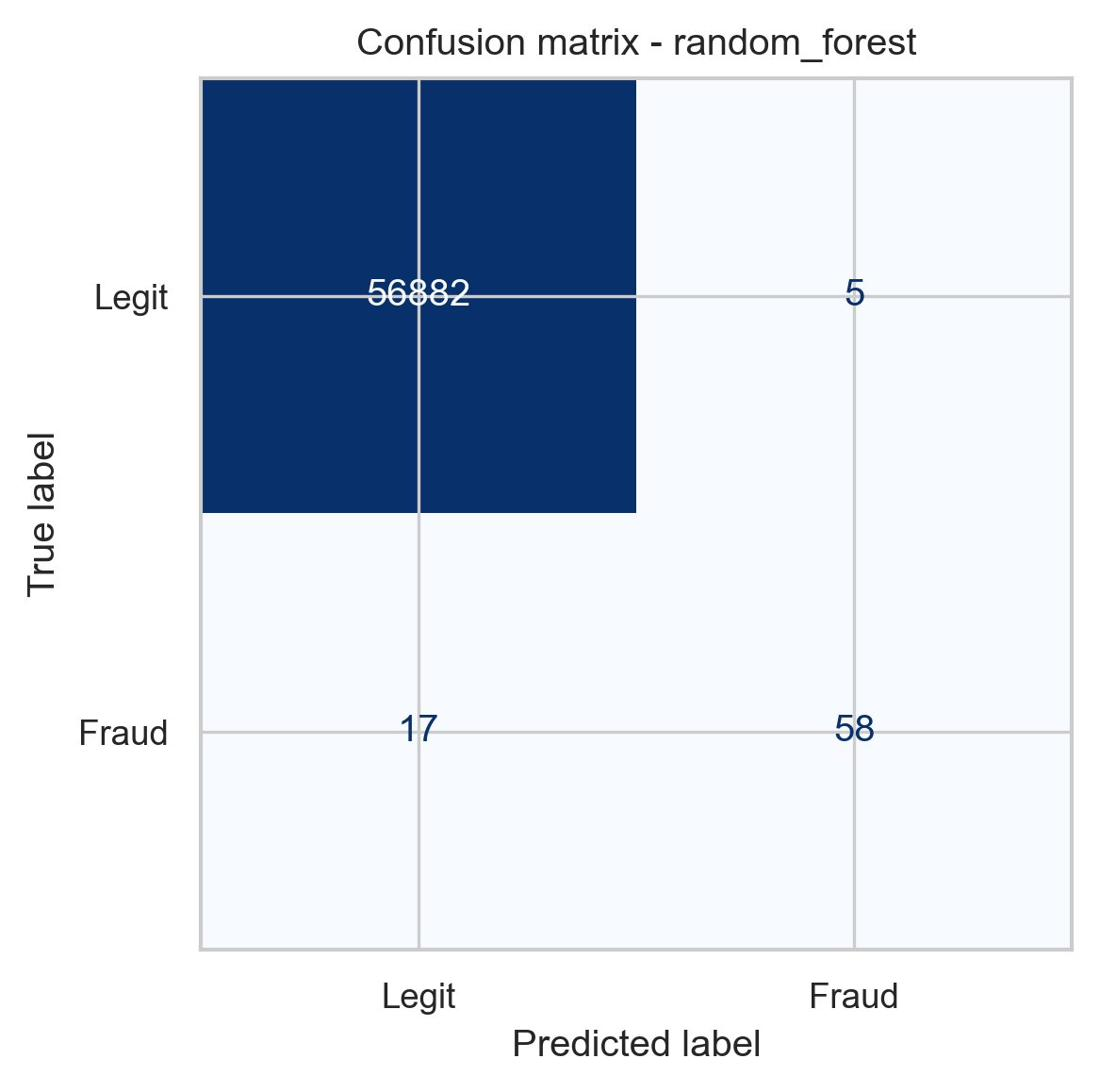
\includegraphics[width=0.92\textwidth]{figures/image5.png}
\end{figure}

\emph{Matrice de confusion — Random Forest (modèle retenu) (jeu de test temporel, }\emph{dataset}\emph{ ULB, seuil optimisé).}

\begin{figure}[H]
\centering
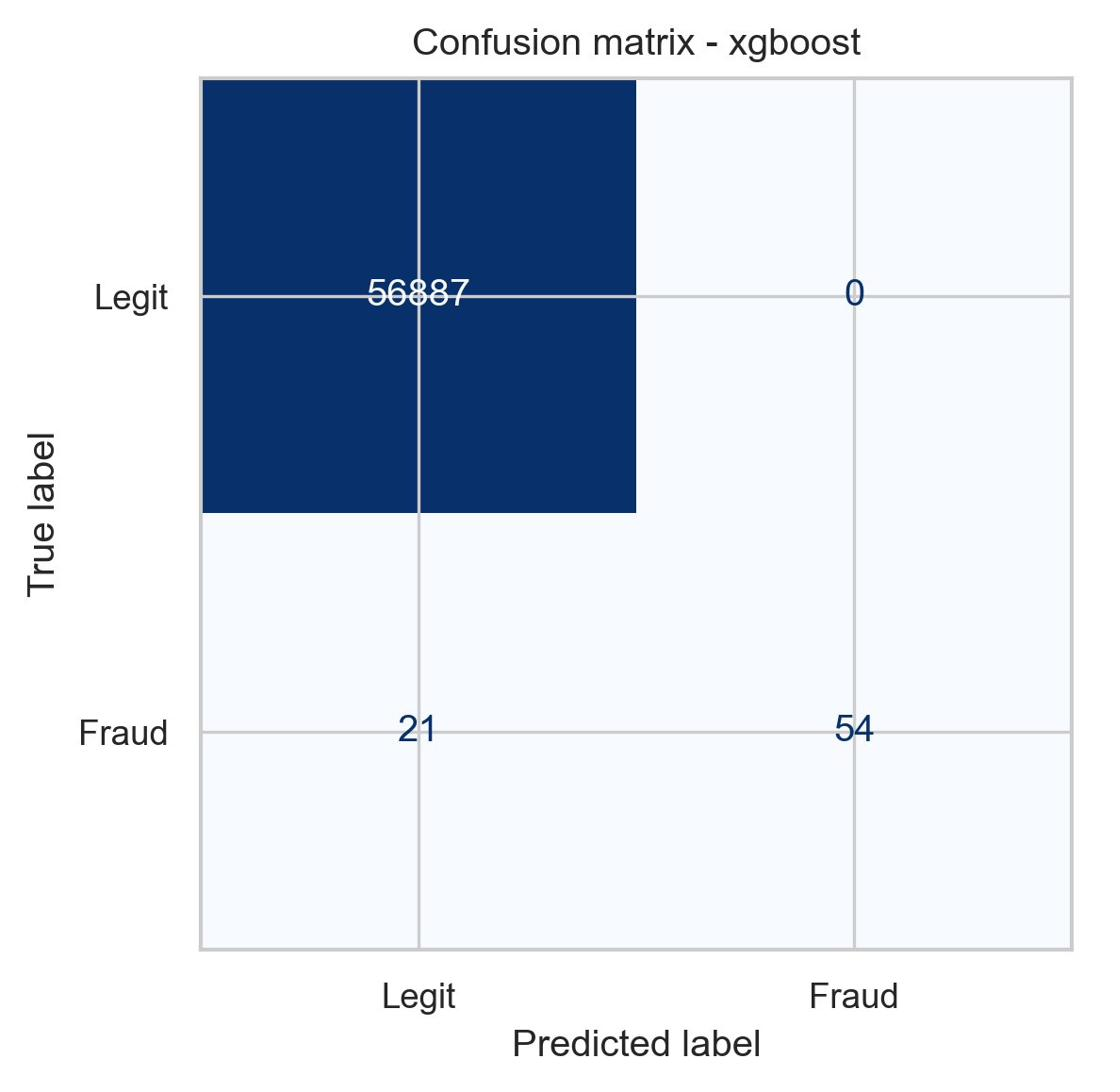
\includegraphics[width=0.92\textwidth]{figures/image6.png}
\end{figure}

\emph{Matrice de confusion — }\emph{XGBoost}\emph{ (jeu de test temporel, }\emph{dataset}\emph{ ULB, seuil optimisé).}

\begin{figure}[H]
\centering
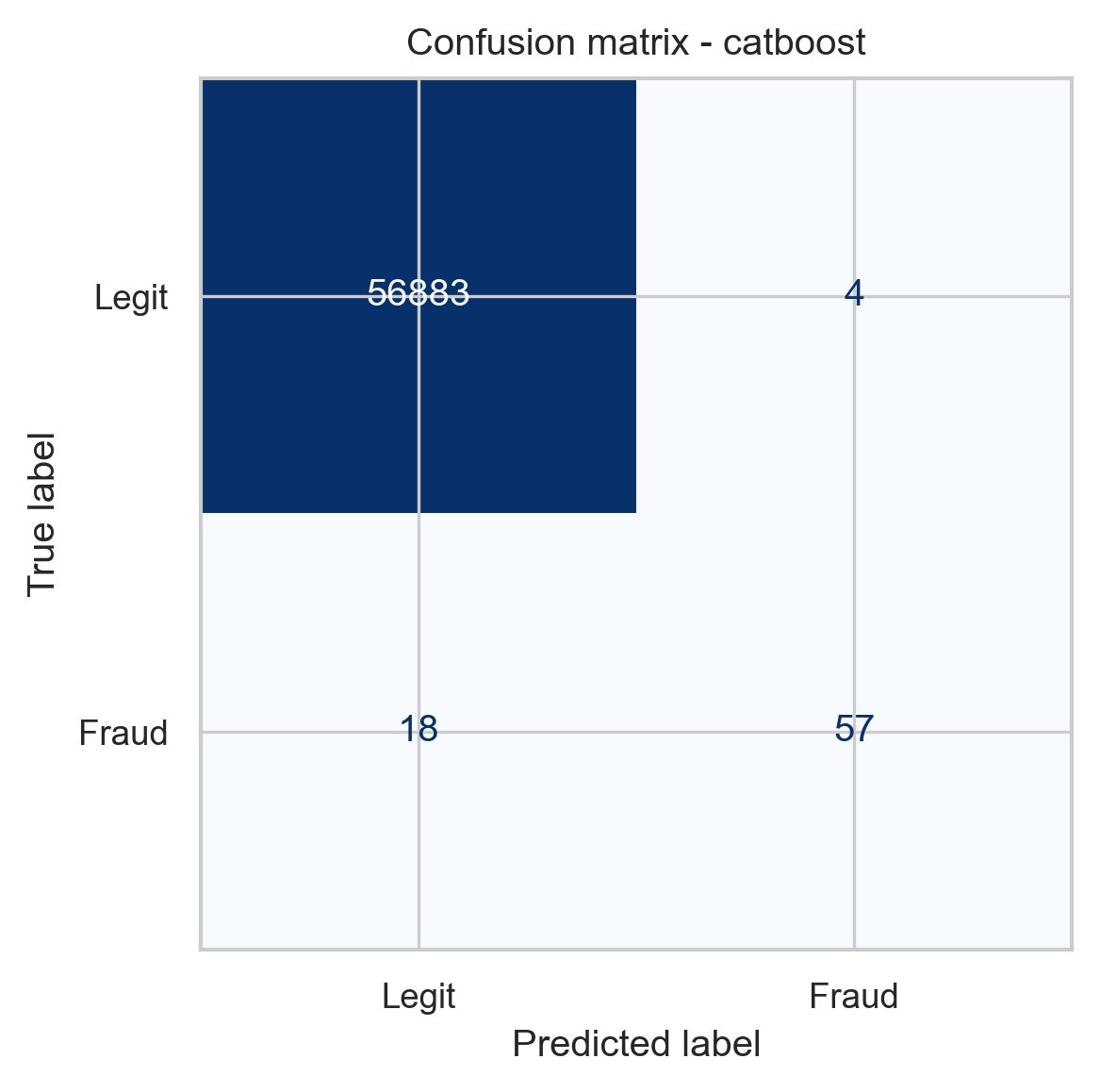
\includegraphics[width=0.92\textwidth]{figures/image7.png}
\end{figure}

\emph{Matrice de confusion — }\emph{CatBoost}\emph{ (jeu de test temporel, }\emph{dataset}\emph{ ULB, seuil optimisé).}

\begin{figure}[H]
\centering
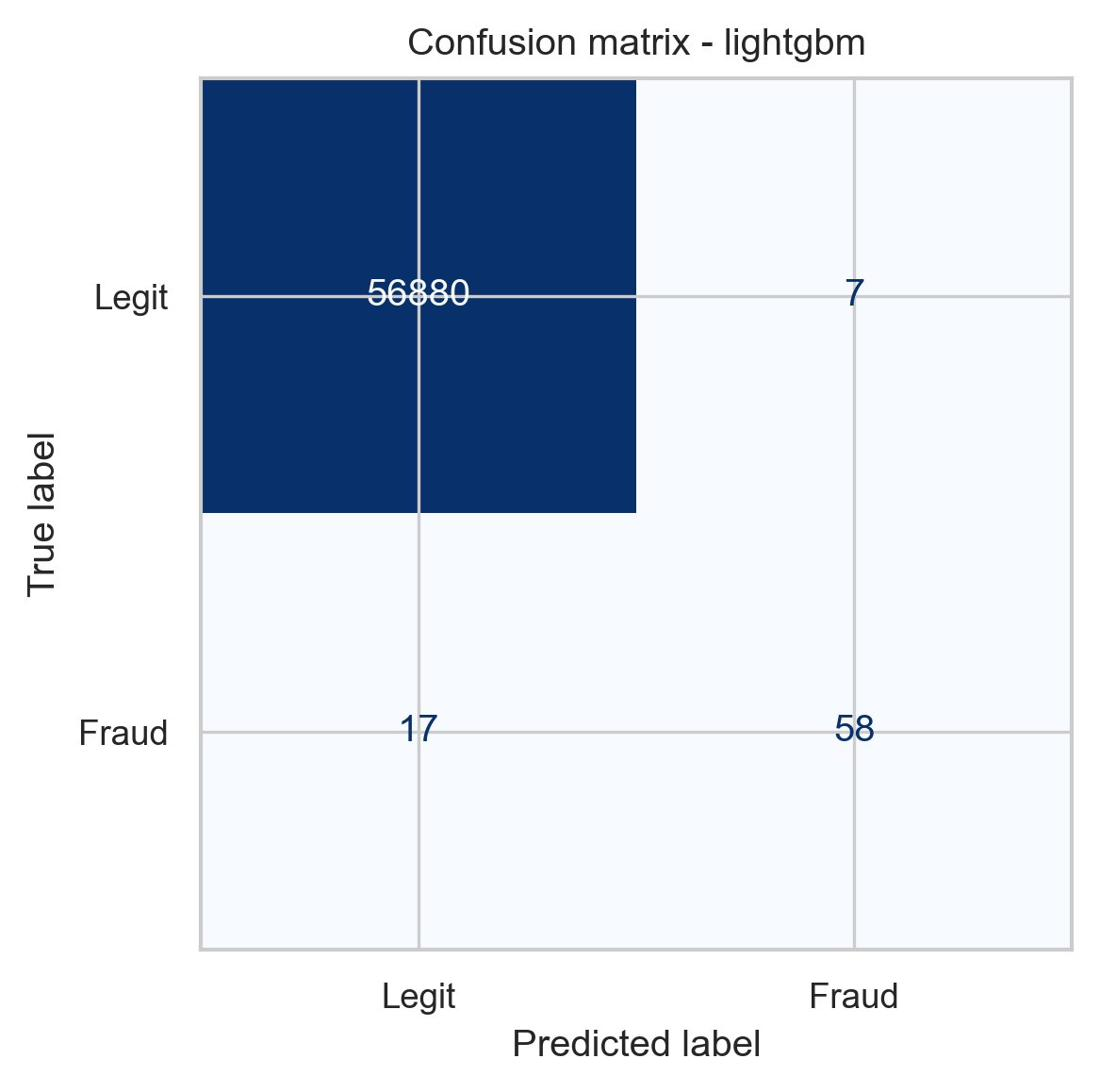
\includegraphics[width=0.92\textwidth]{figures/image17.png}
\end{figure}

\emph{Matrice de confusion — }\emph{LightGBM}\emph{ (jeu de test temporel, }\emph{dataset}\emph{ ULB, seuil optimisé).}

\begin{figure}[H]
\centering
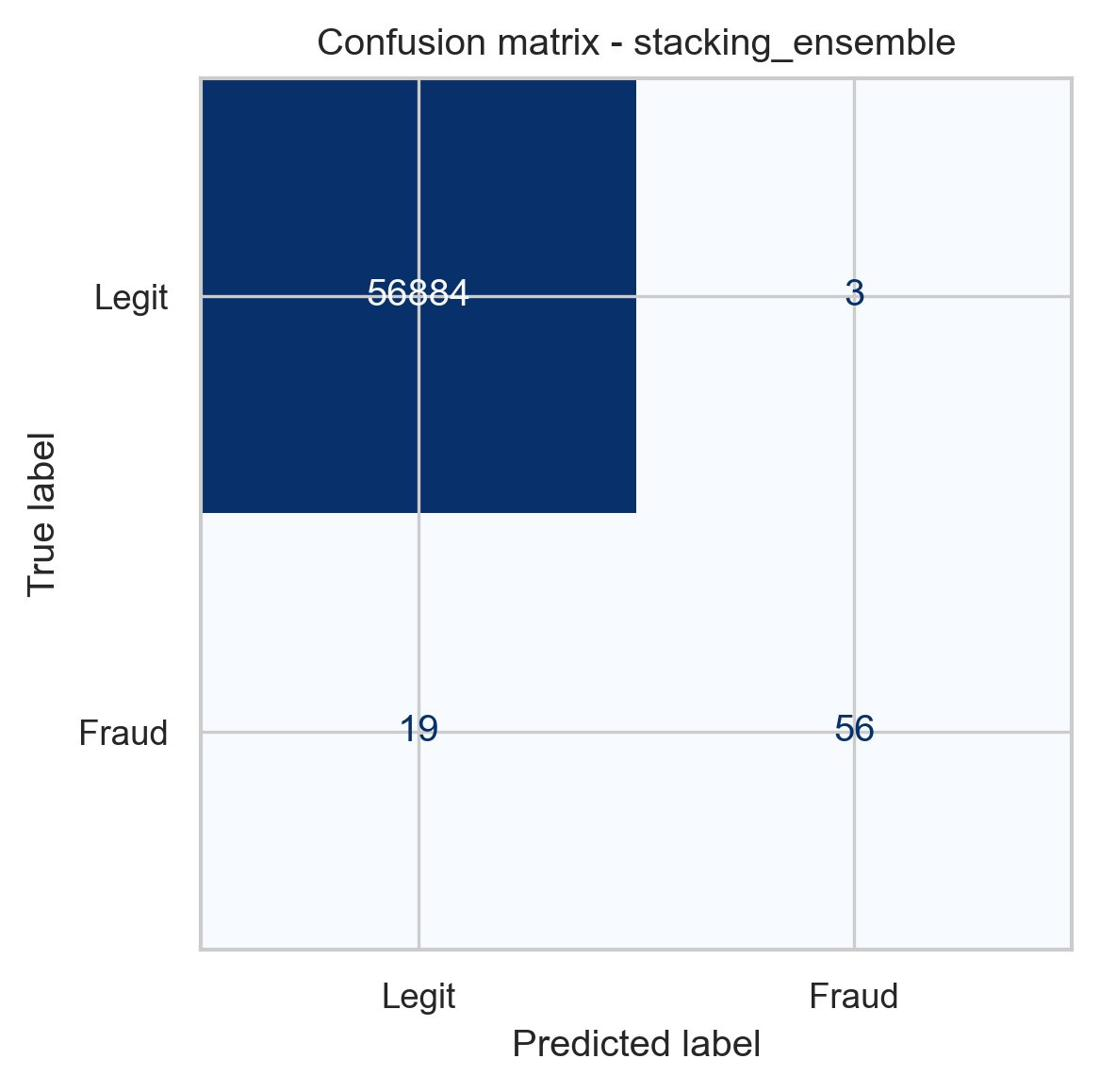
\includegraphics[width=0.92\textwidth]{figures/image8.png}
\end{figure}

\emph{Matrice de confusion — }\emph{Stacking}\emph{ Ensemble (méta LR) (jeu de test temporel, }\emph{dataset}\emph{ ULB, seuil optimisé).}

\begin{figure}[H]
\centering
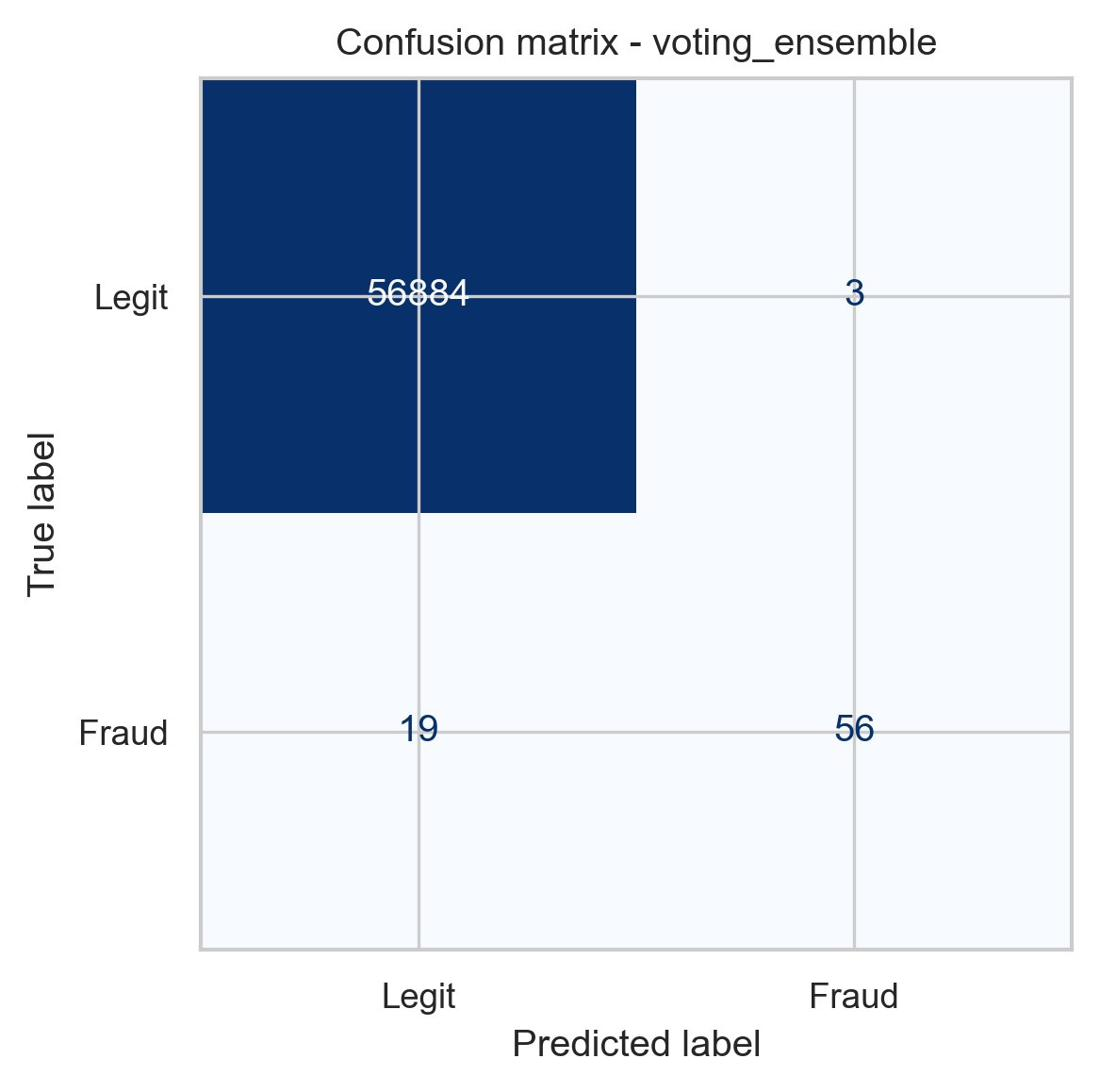
\includegraphics[width=0.92\textwidth]{figures/image18.png}
\end{figure}

\emph{Matrice de confusion — }\emph{Voting}\emph{ Soft (jeu de test temporel, }\emph{dataset}\emph{ ULB, seuil optimisé).}

\begin{figure}[H]
\centering
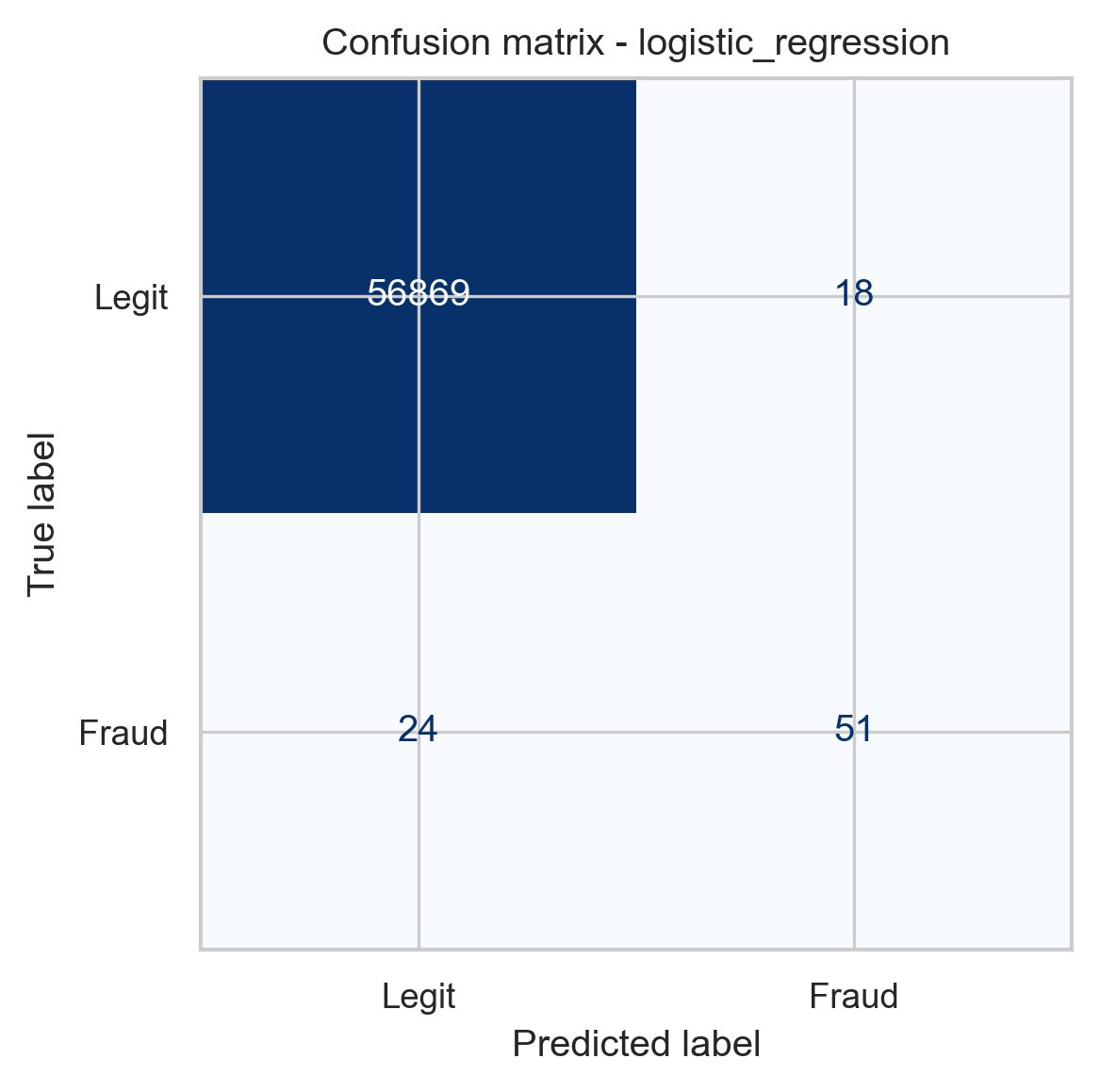
\includegraphics[width=0.92\textwidth]{figures/image19.png}
\end{figure}

\emph{Matrice de confusion — Régression Logistique (}\emph{baseline}\emph{) (jeu de test temporel, }\emph{dataset}\emph{ ULB, seuil optimisé).}

\textbf{B.2. Courbes coût total en fonction du seuil — tous les modèles}

Les courbes suivantes montrent l'évolution du coût total C(s) = FN(s)·C\_FN + FP(s)·C\_FP en fonction du seuil pour chaque modèle, permettant d'identifier le seuil optimal coût-sensible.

\begin{figure}[H]
\centering
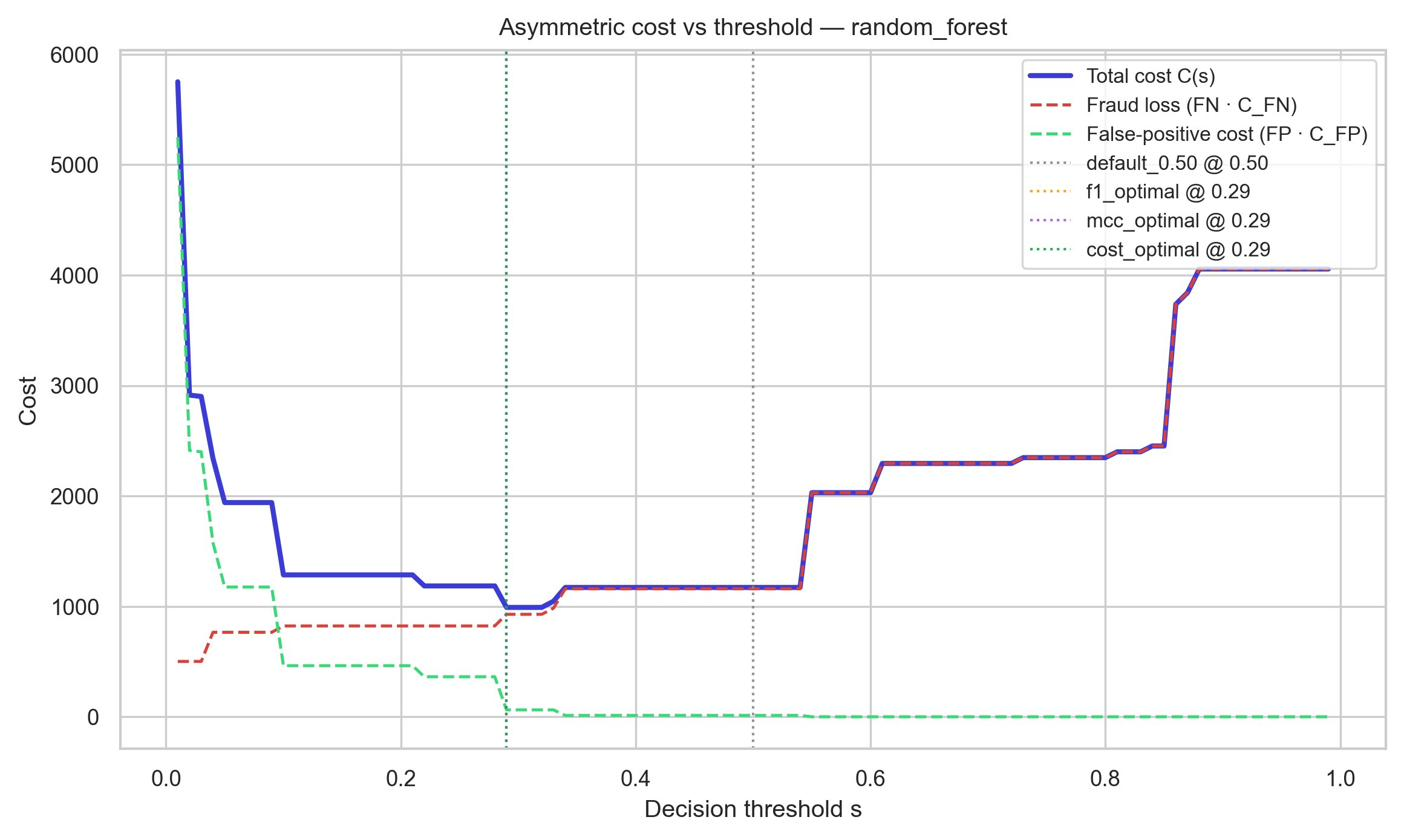
\includegraphics[width=0.92\textwidth]{figures/image11.png}
\end{figure}

\emph{Courbe coût/seuil — Random Forest (modèle retenu) (jeu de test temporel, }\emph{dataset}\emph{ ULB).}

\begin{figure}[H]
\centering
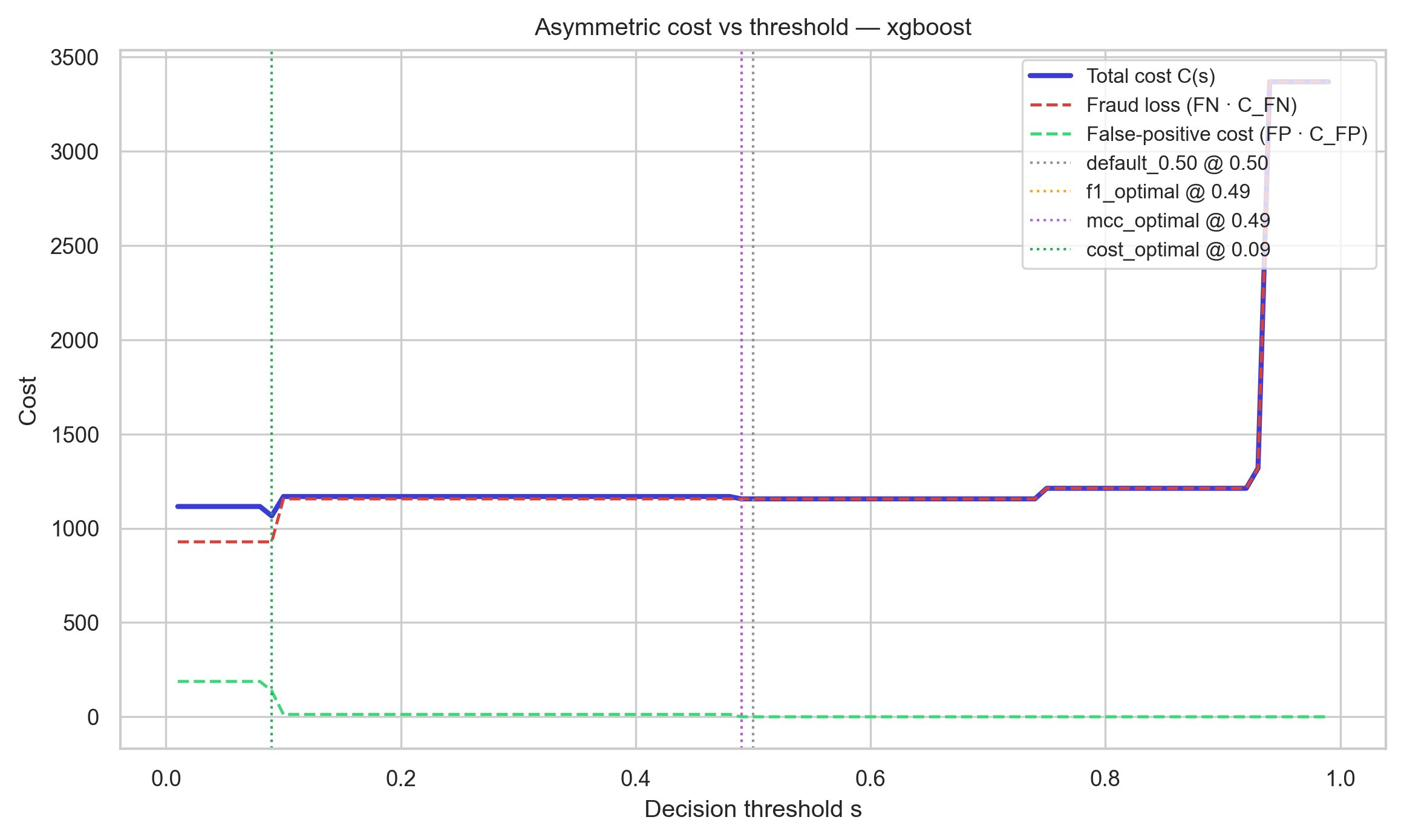
\includegraphics[width=0.92\textwidth]{figures/image12.png}
\end{figure}

\emph{Courbe coût/seuil — }\emph{XGBoost}\emph{ (jeu de test temporel, }\emph{dataset}\emph{ ULB).}

\begin{figure}[H]
\centering
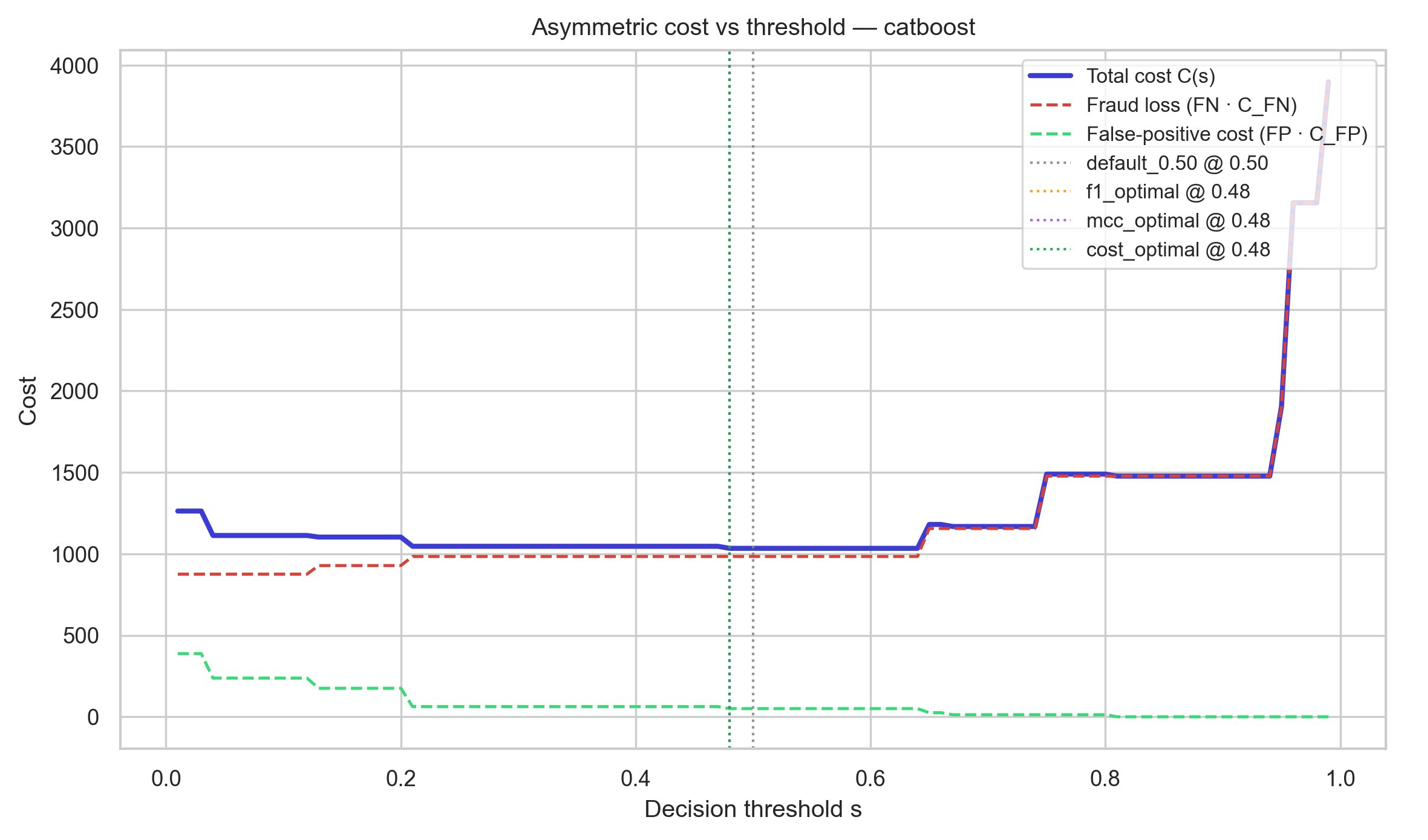
\includegraphics[width=0.92\textwidth]{figures/image20.png}
\end{figure}

\emph{Courbe coût/seuil — }\emph{CatBoost}\emph{ (jeu de test temporel, }\emph{dataset}\emph{ ULB).}

\begin{figure}[H]
\centering
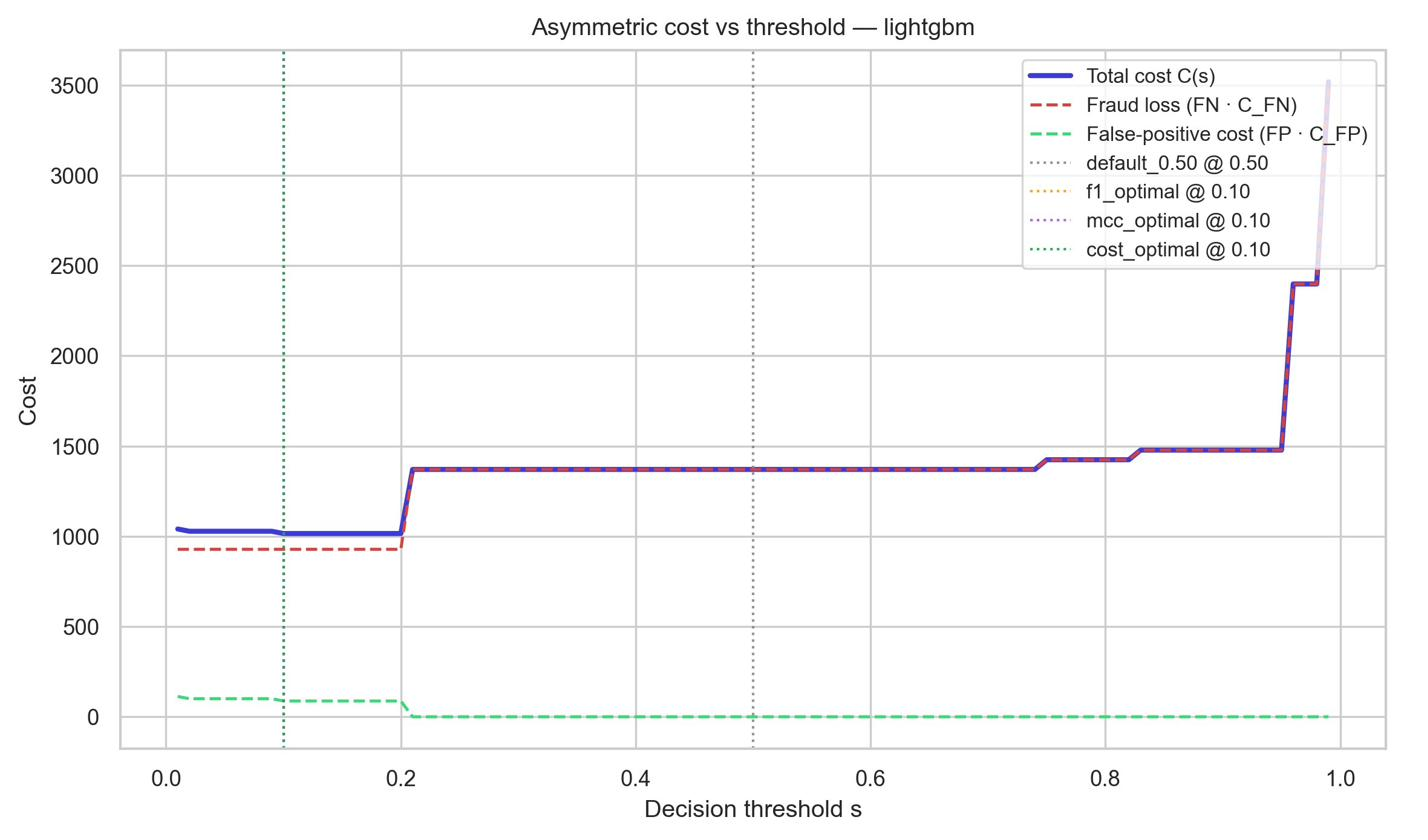
\includegraphics[width=0.92\textwidth]{figures/image21.png}
\end{figure}

\emph{Courbe coût/seuil — }\emph{LightGBM}\emph{ (jeu de test temporel, }\emph{dataset}\emph{ ULB).}

\begin{figure}[H]
\centering
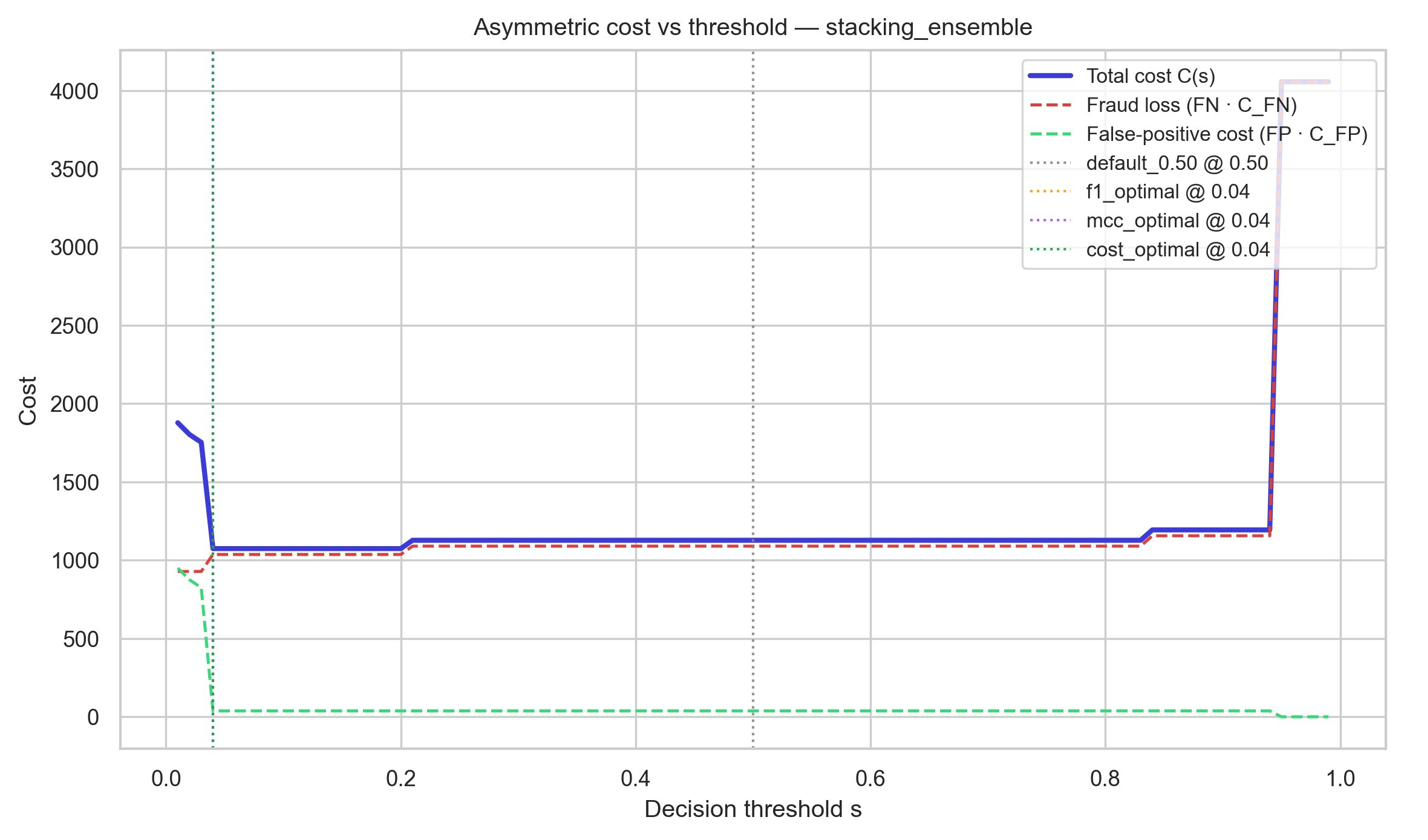
\includegraphics[width=0.92\textwidth]{figures/image13.png}
\end{figure}

\emph{Courbe coût/seuil — }\emph{Stacking}\emph{ Ensemble (jeu de test temporel, }\emph{dataset}\emph{ ULB).}

\begin{figure}[H]
\centering
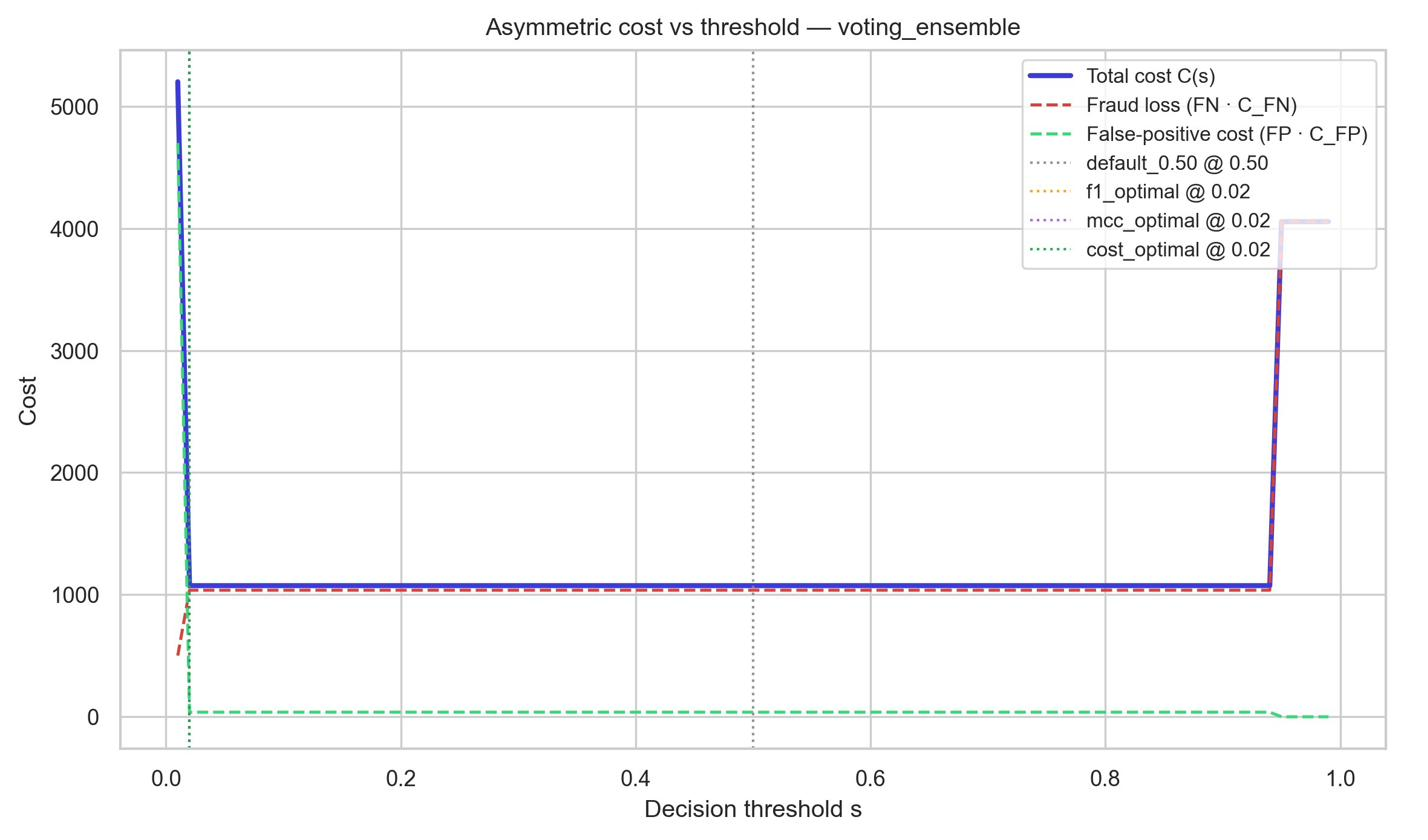
\includegraphics[width=0.92\textwidth]{figures/image22.png}
\end{figure}

\emph{Courbe coût/seuil — }\emph{Voting}\emph{ Soft (jeu de test temporel, }\emph{dataset}\emph{ ULB).}

\begin{figure}[H]
\centering
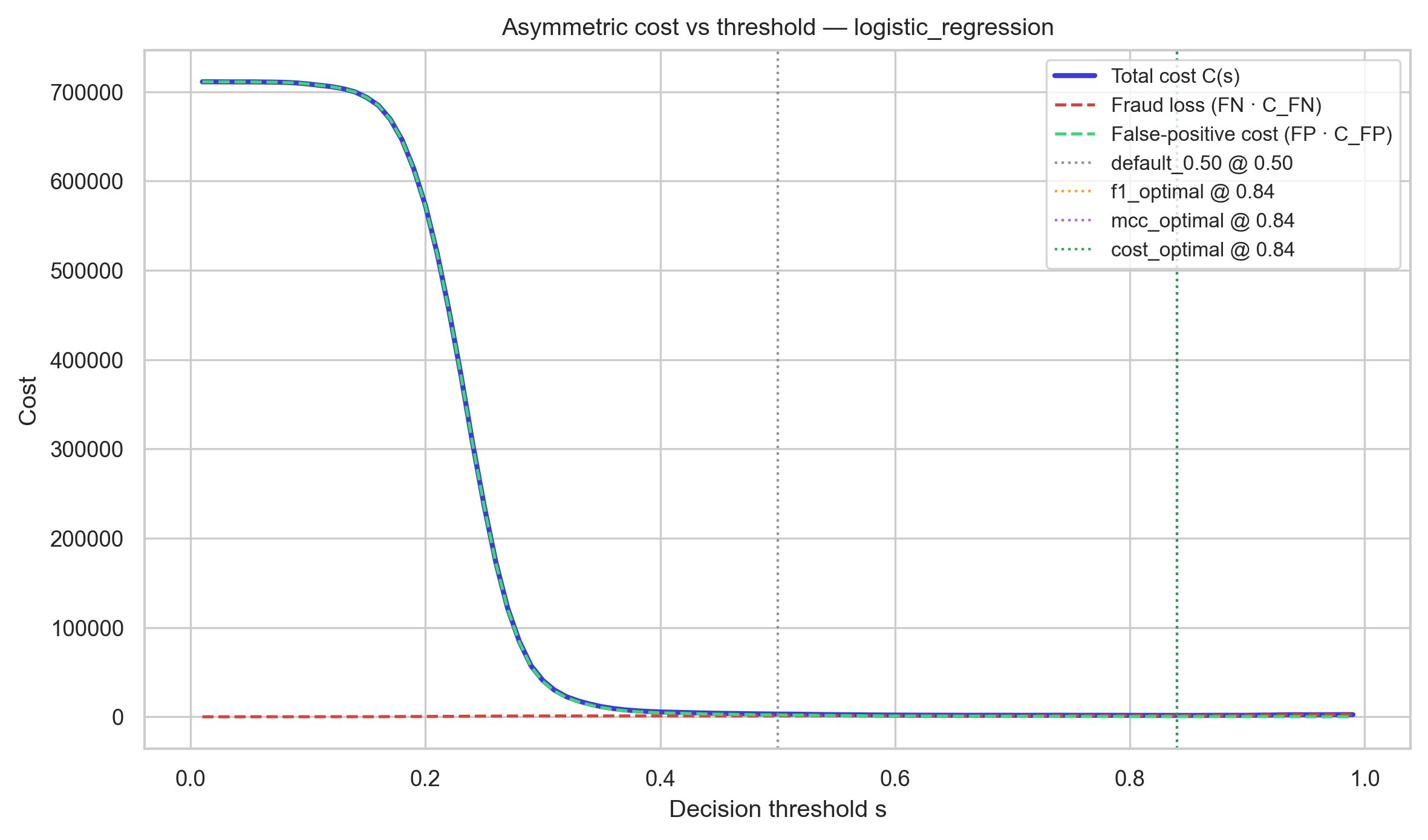
\includegraphics[width=0.92\textwidth]{figures/image23.png}
\end{figure}

\emph{Courbe coût/seuil — Régression Logistique (}\emph{baseline}\emph{) (jeu de test temporel, }\emph{dataset}\emph{ ULB).}

\textbf{B.3. Courbes seuil / métriques et gains économiques — tous les modèles}

\begin{figure}[H]
\centering
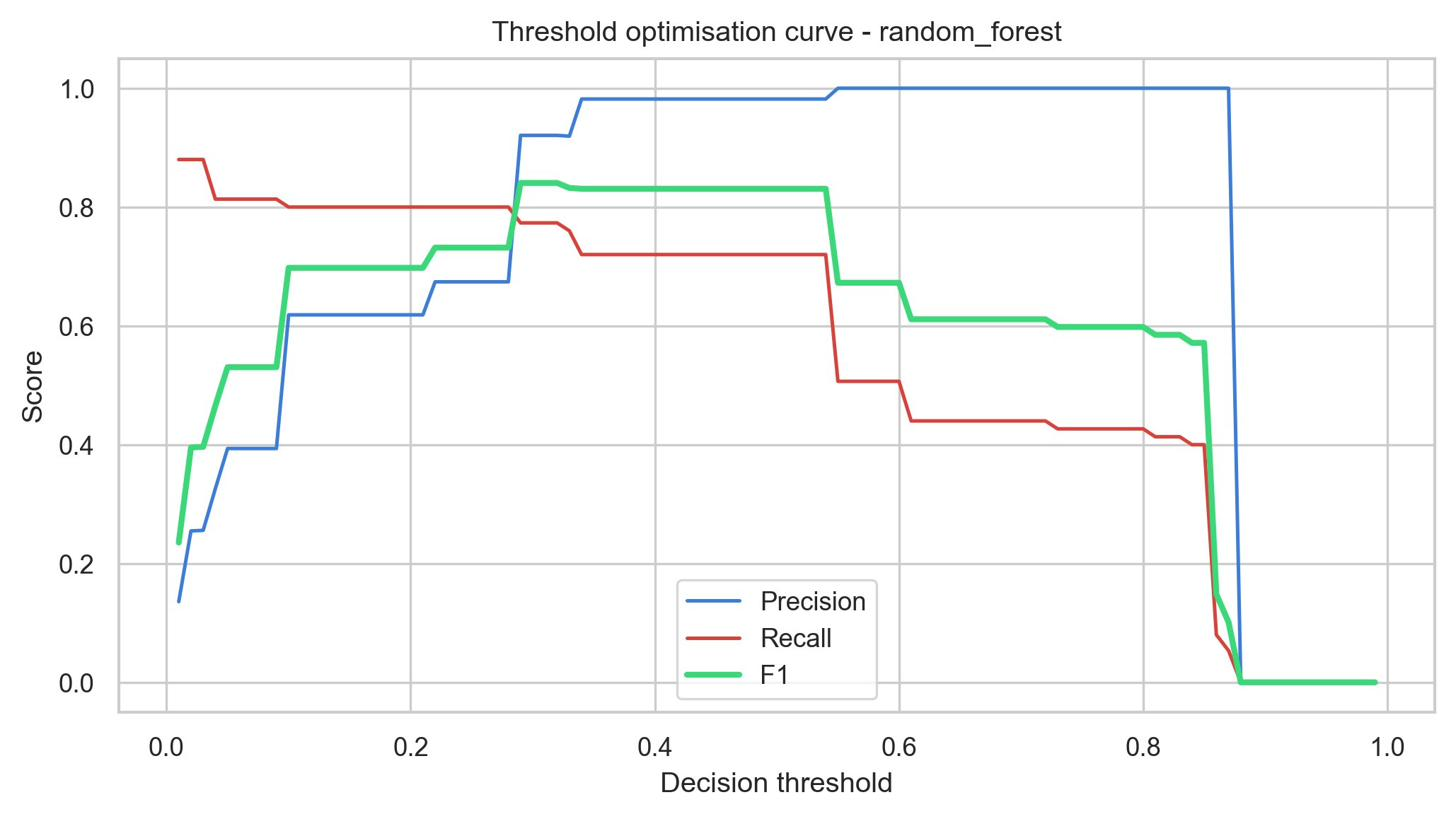
\includegraphics[width=0.92\textwidth]{figures/image10.png}
\end{figure}

\emph{Seuil/métriques — Random Forest.}

\begin{figure}[H]
\centering
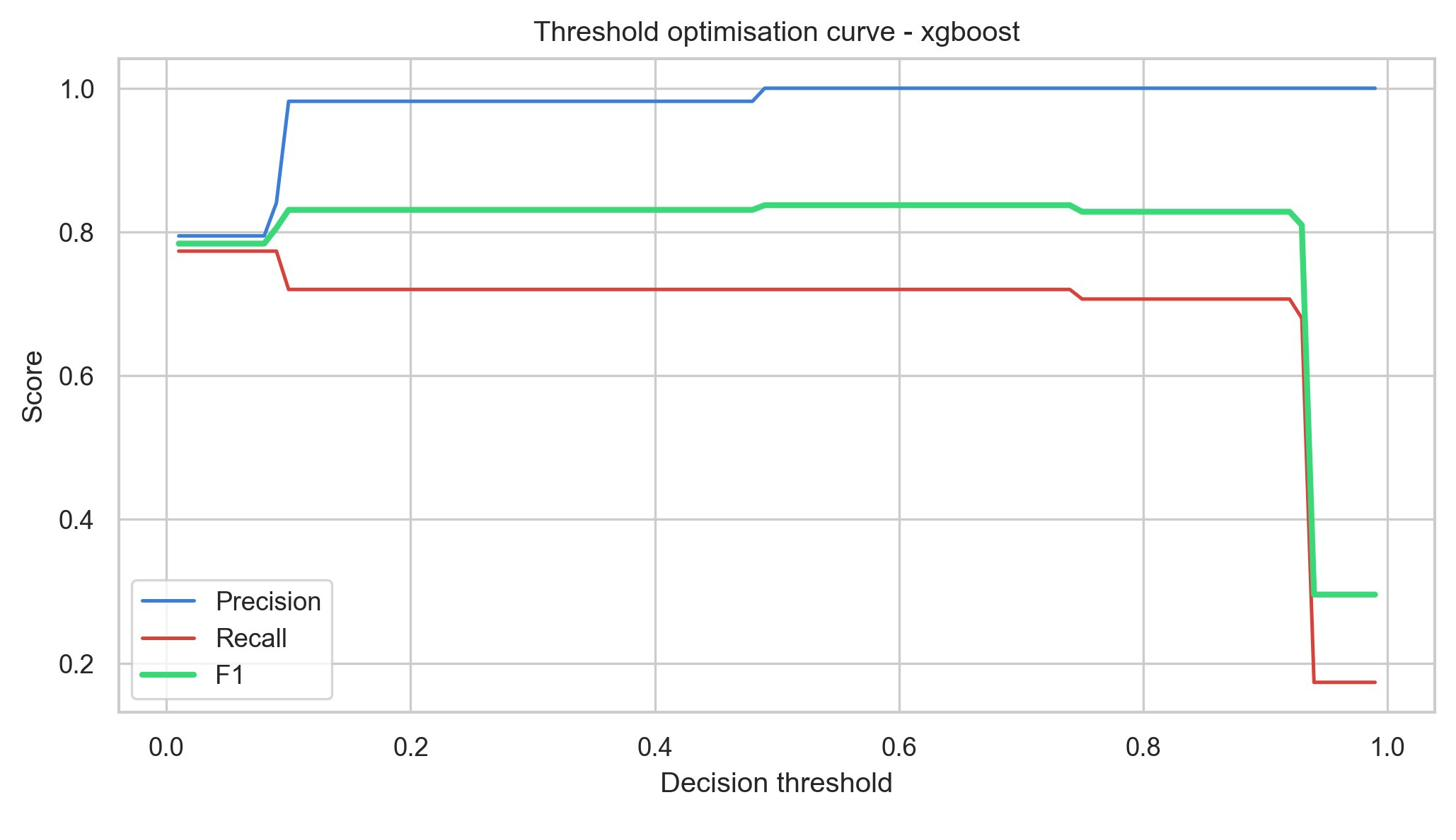
\includegraphics[width=0.92\textwidth]{figures/image24.png}
\end{figure}

\emph{Seuil/métriques — }\emph{XGBoost}\emph{.}

\begin{figure}[H]
\centering
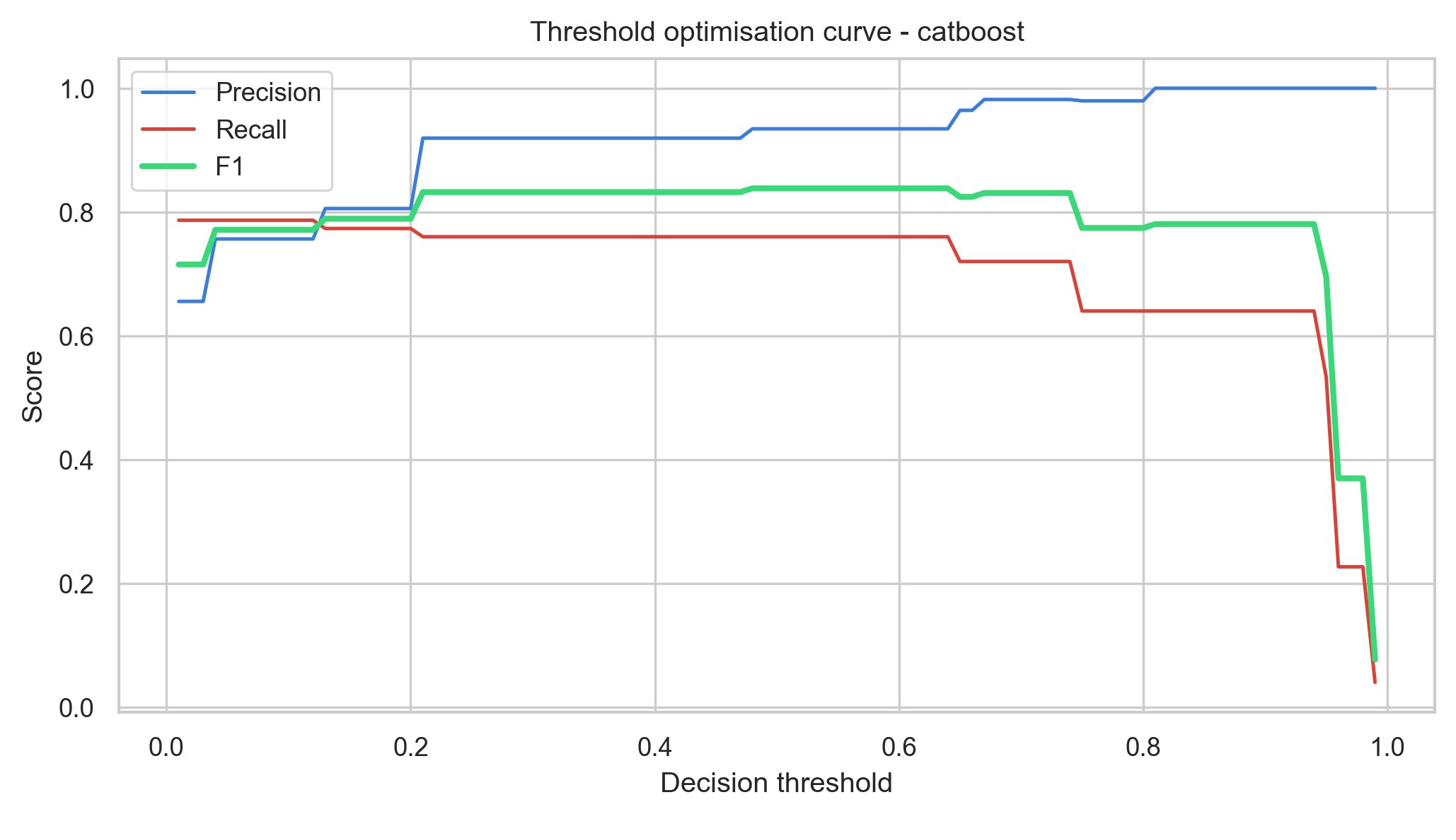
\includegraphics[width=0.92\textwidth]{figures/image25.png}
\end{figure}

\emph{Seuil/métriques — }\emph{CatBoost}\emph{.}

\begin{figure}[H]
\centering
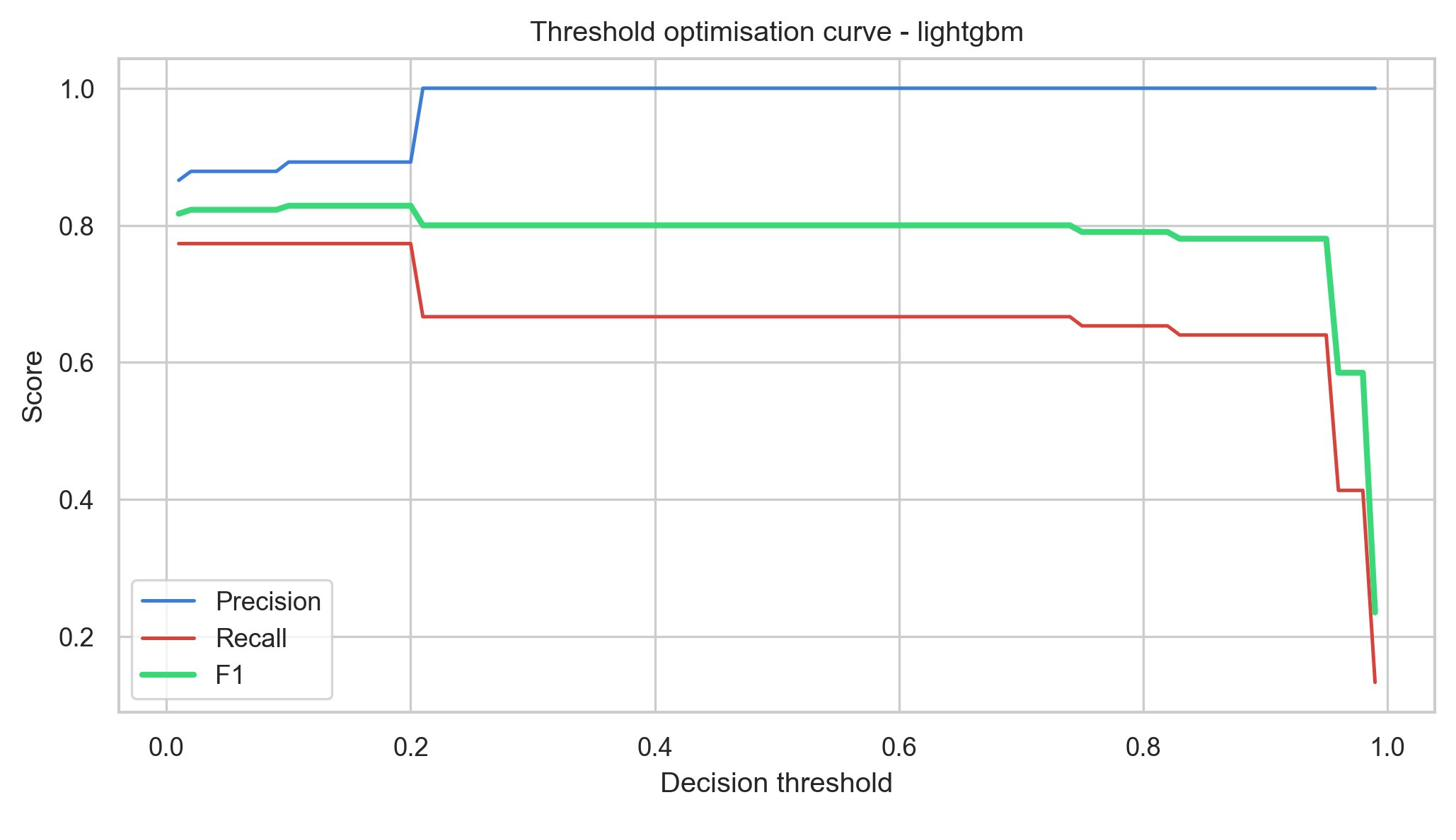
\includegraphics[width=0.92\textwidth]{figures/image26.png}
\end{figure}

\emph{Seuil/métriques — }\emph{LightGBM}\emph{.}

\begin{figure}[H]
\centering
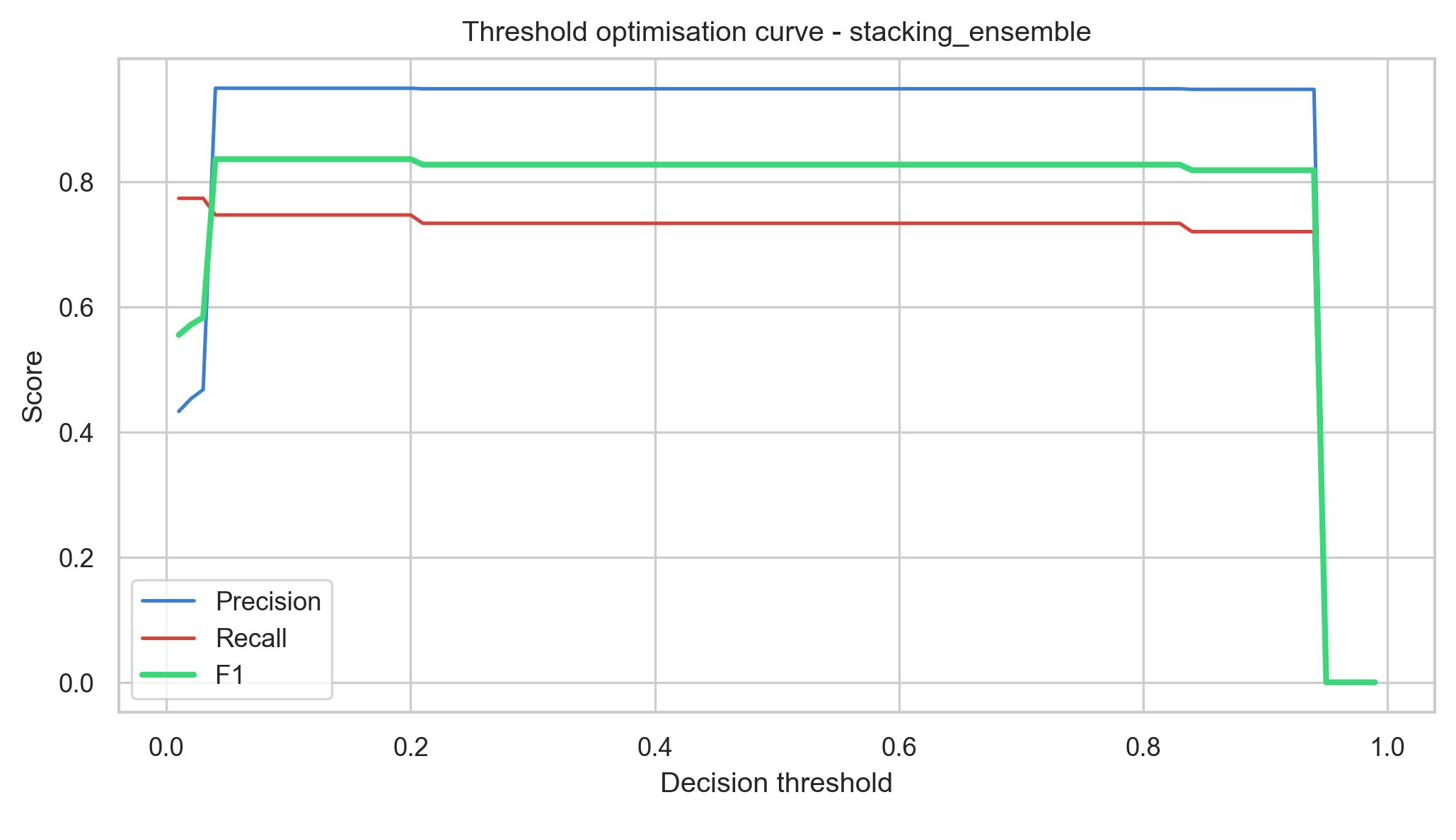
\includegraphics[width=0.92\textwidth]{figures/image27.png}
\end{figure}

\emph{Seuil/métriques — }\emph{Stacking}\emph{ Ensemble.}

\begin{figure}[H]
\centering
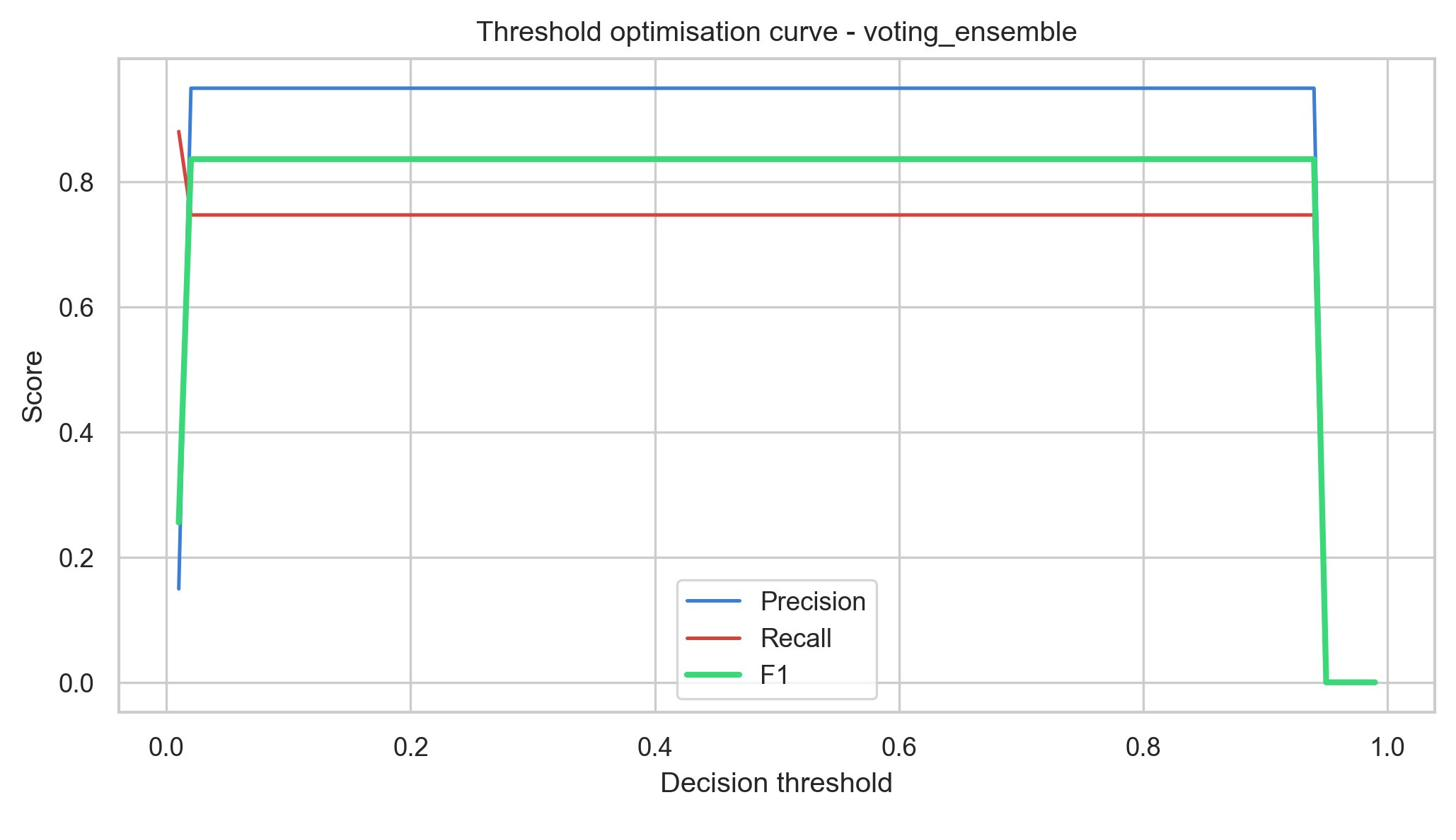
\includegraphics[width=0.92\textwidth]{figures/image28.png}
\end{figure}

\emph{Seuil/métriques — }\emph{Voting}\emph{ Soft.}

\begin{figure}[H]
\centering
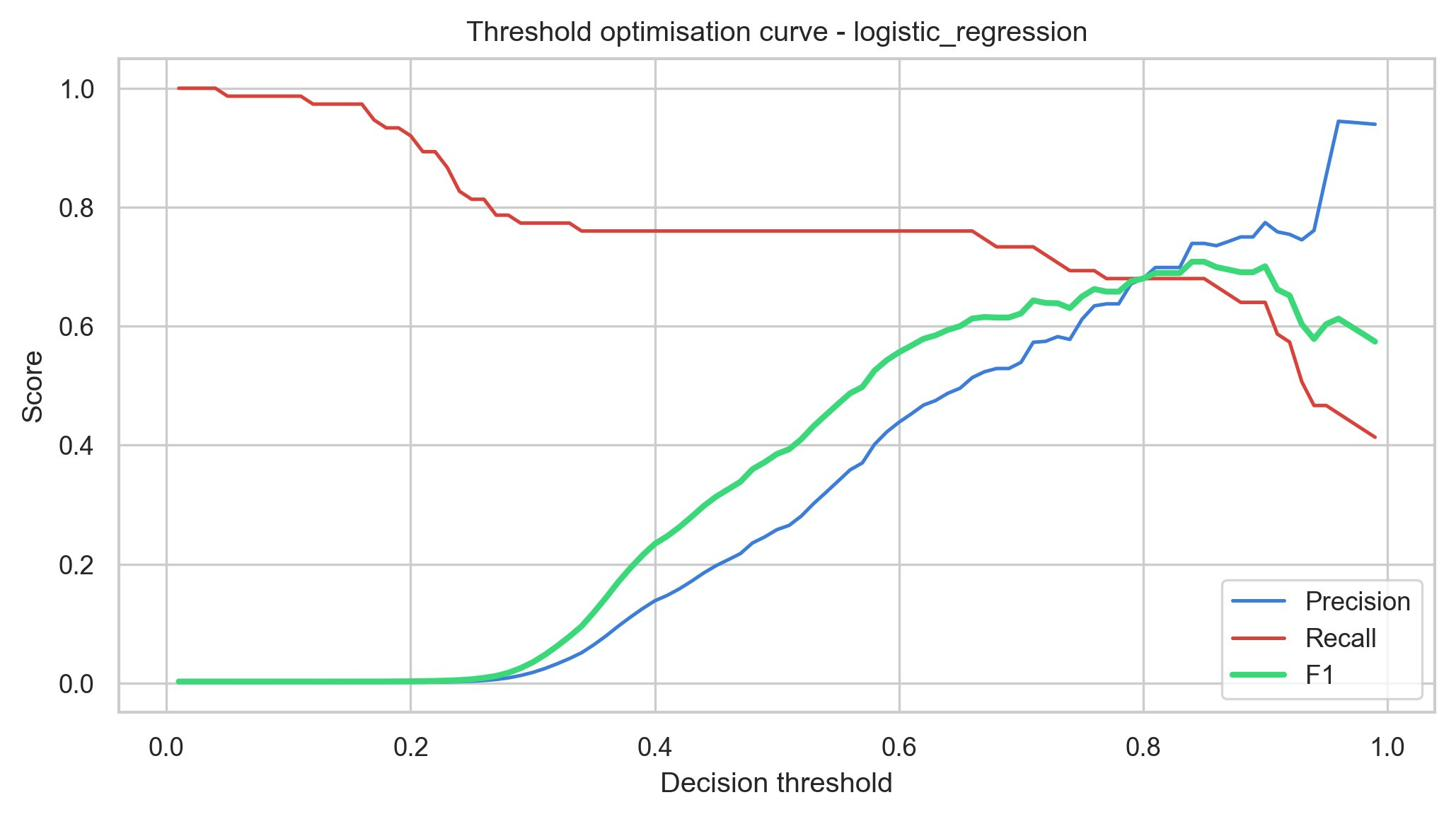
\includegraphics[width=0.92\textwidth]{figures/image29.png}
\end{figure}

\emph{Seuil/métriques — Régression Logistique.}

\begin{figure}[H]
\centering
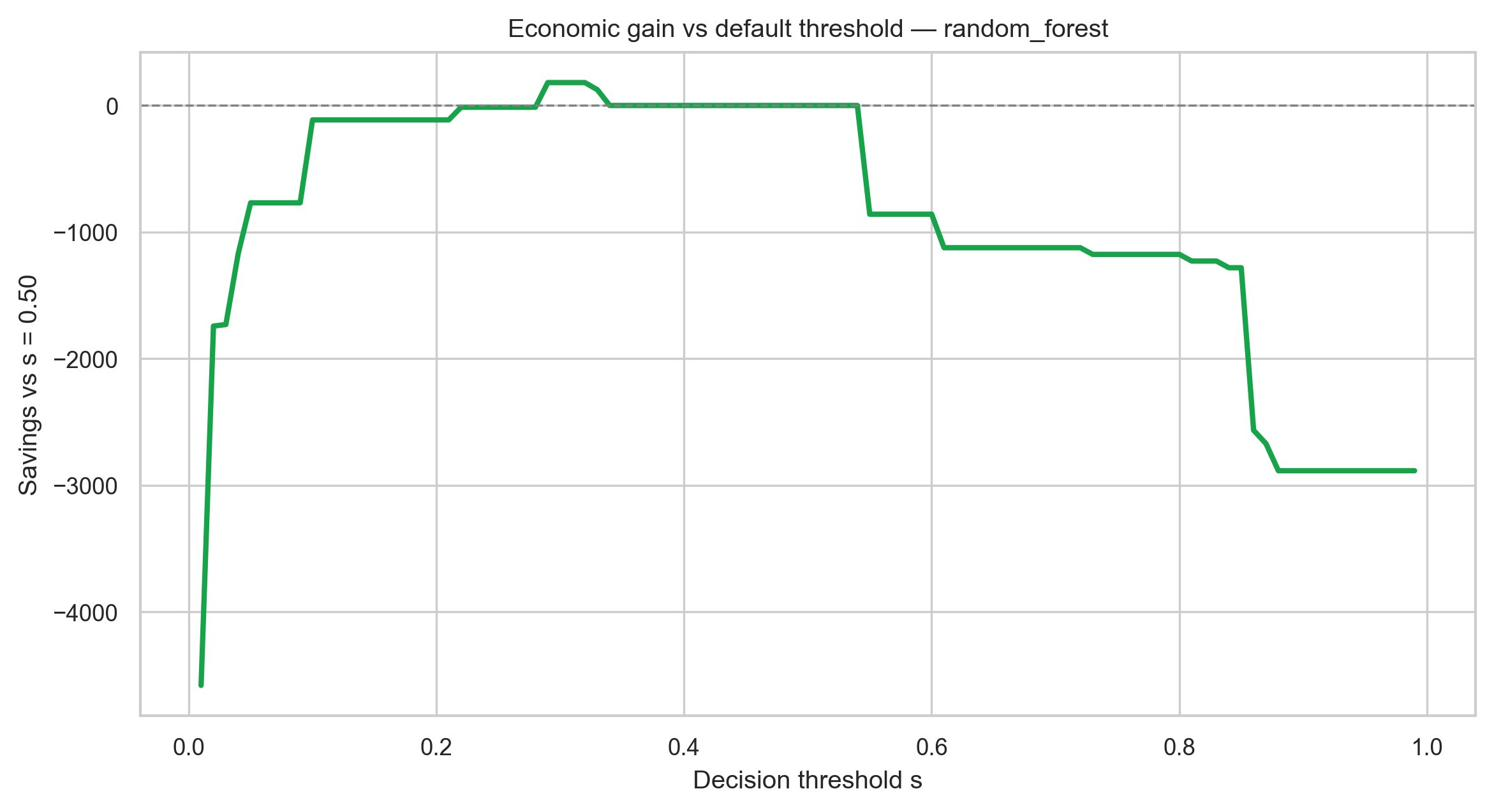
\includegraphics[width=0.92\textwidth]{figures/image16.png}
\end{figure}

\emph{Gains économiques — Random Forest.}

\begin{figure}[H]
\centering
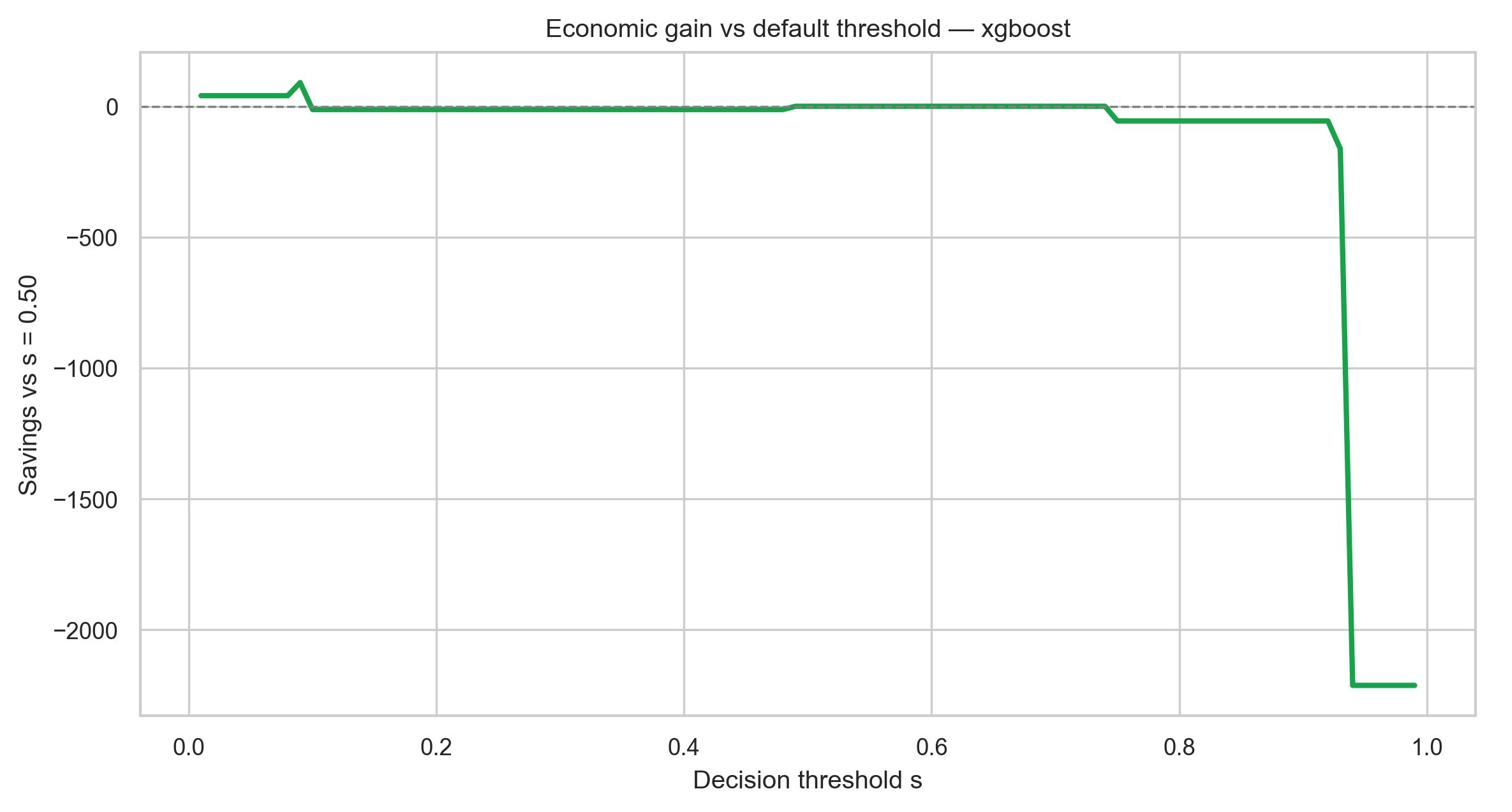
\includegraphics[width=0.92\textwidth]{figures/image30.png}
\end{figure}

\emph{Gains économiques — }\emph{XGBoost}\emph{.}

\begin{figure}[H]
\centering
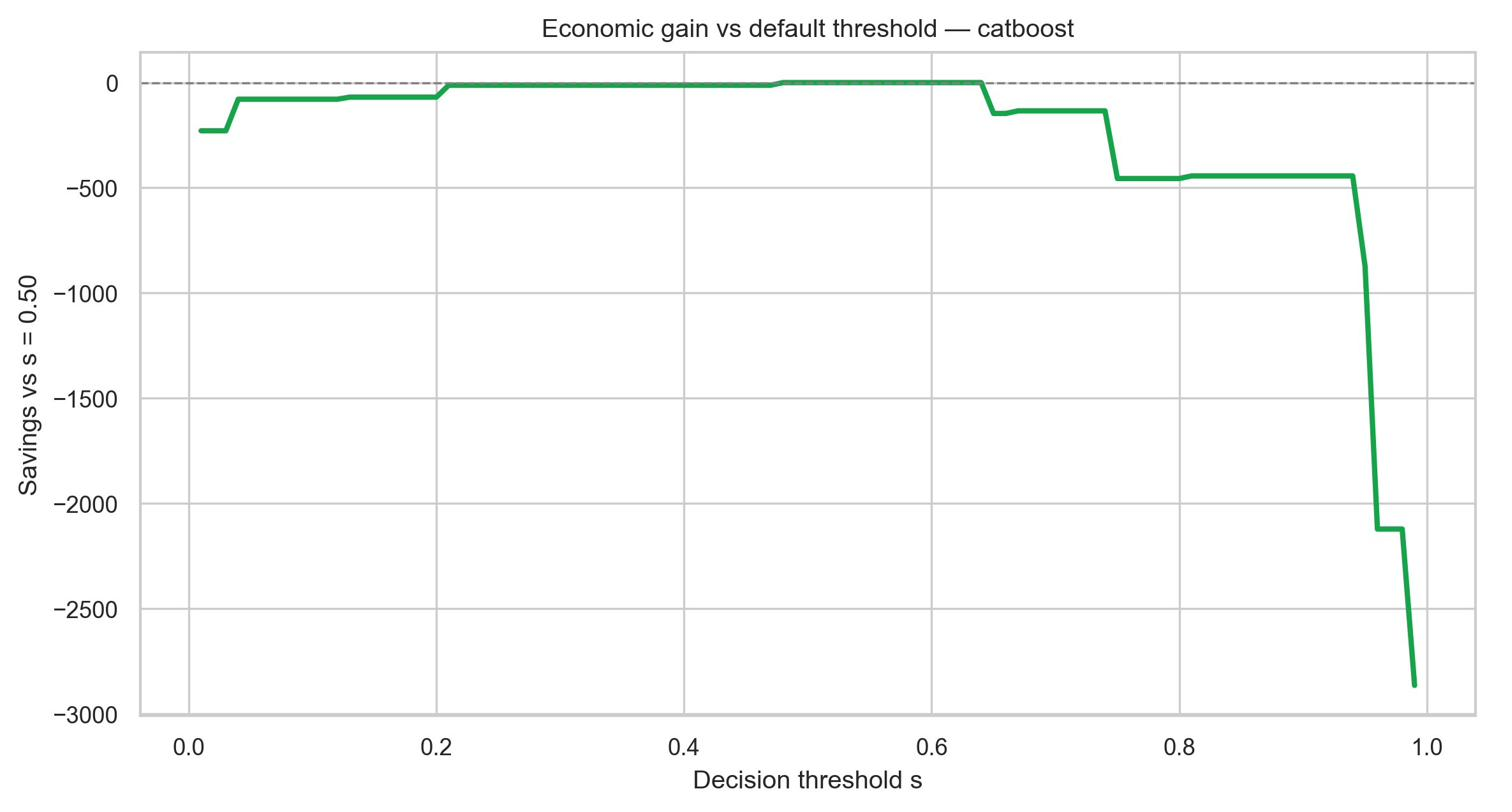
\includegraphics[width=0.92\textwidth]{figures/image31.png}
\end{figure}

\emph{Gains économiques — }\emph{CatBoost}\emph{.}

\begin{figure}[H]
\centering
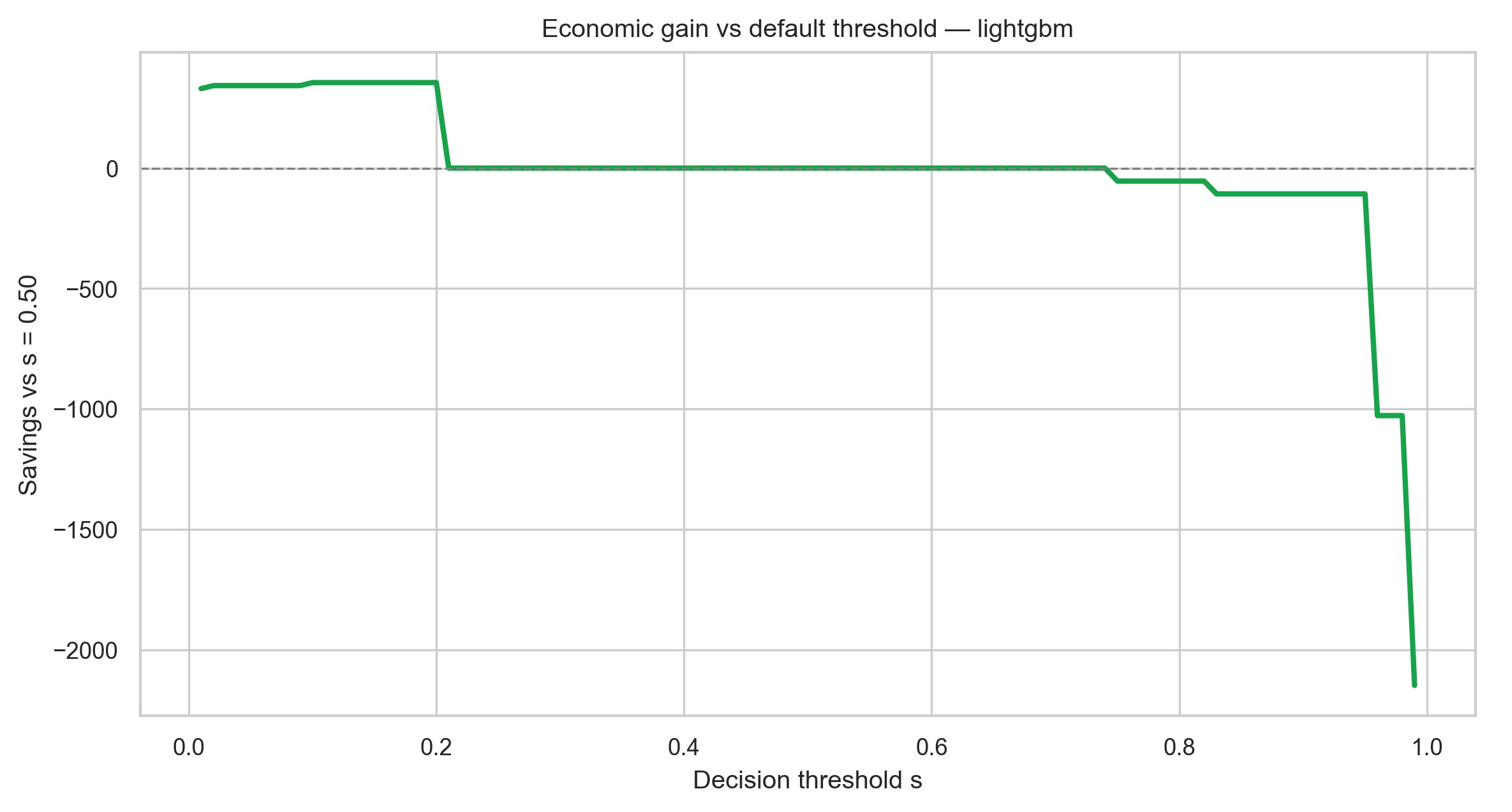
\includegraphics[width=0.92\textwidth]{figures/image32.png}
\end{figure}

\emph{Gains économiques — }\emph{LightGBM}\emph{.}

\begin{figure}[H]
\centering
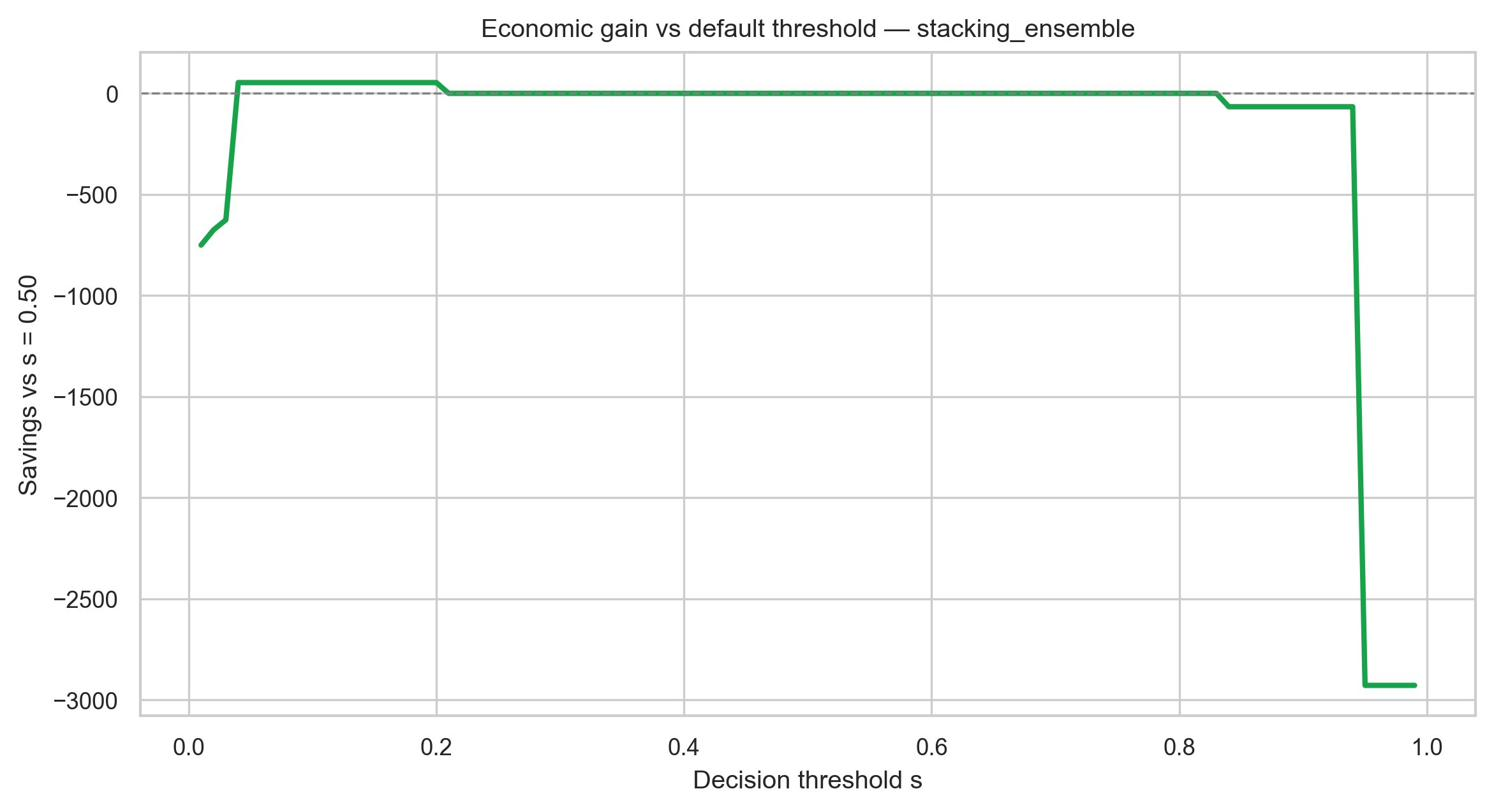
\includegraphics[width=0.92\textwidth]{figures/image33.png}
\end{figure}

\emph{Gains économiques — }\emph{Stacking}\emph{ Ensemble.}

\begin{figure}[H]
\centering
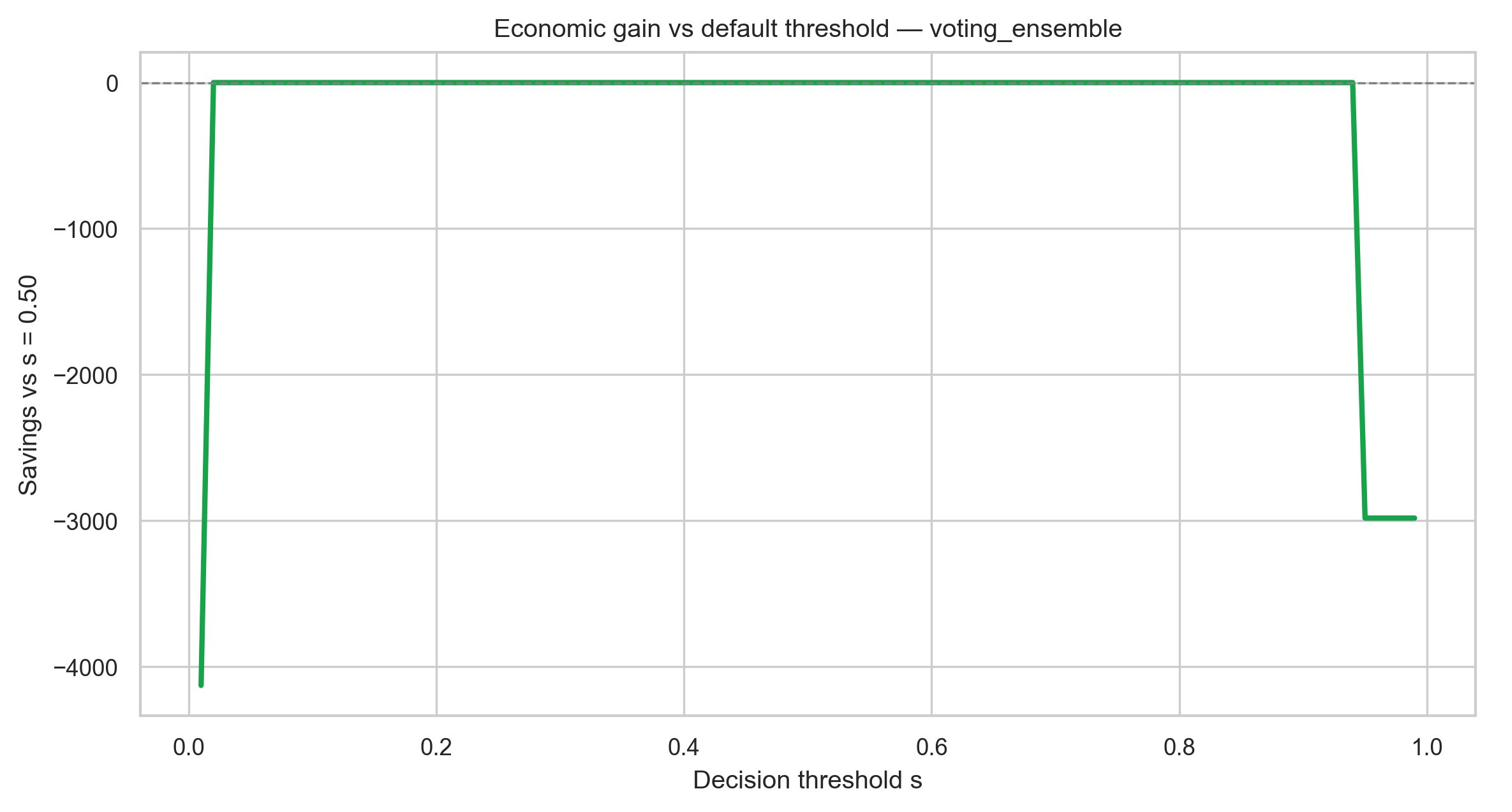
\includegraphics[width=0.92\textwidth]{figures/image34.png}
\end{figure}

\emph{Gains économiques — }\emph{Voting}\emph{ Soft.}

\begin{figure}[H]
\centering
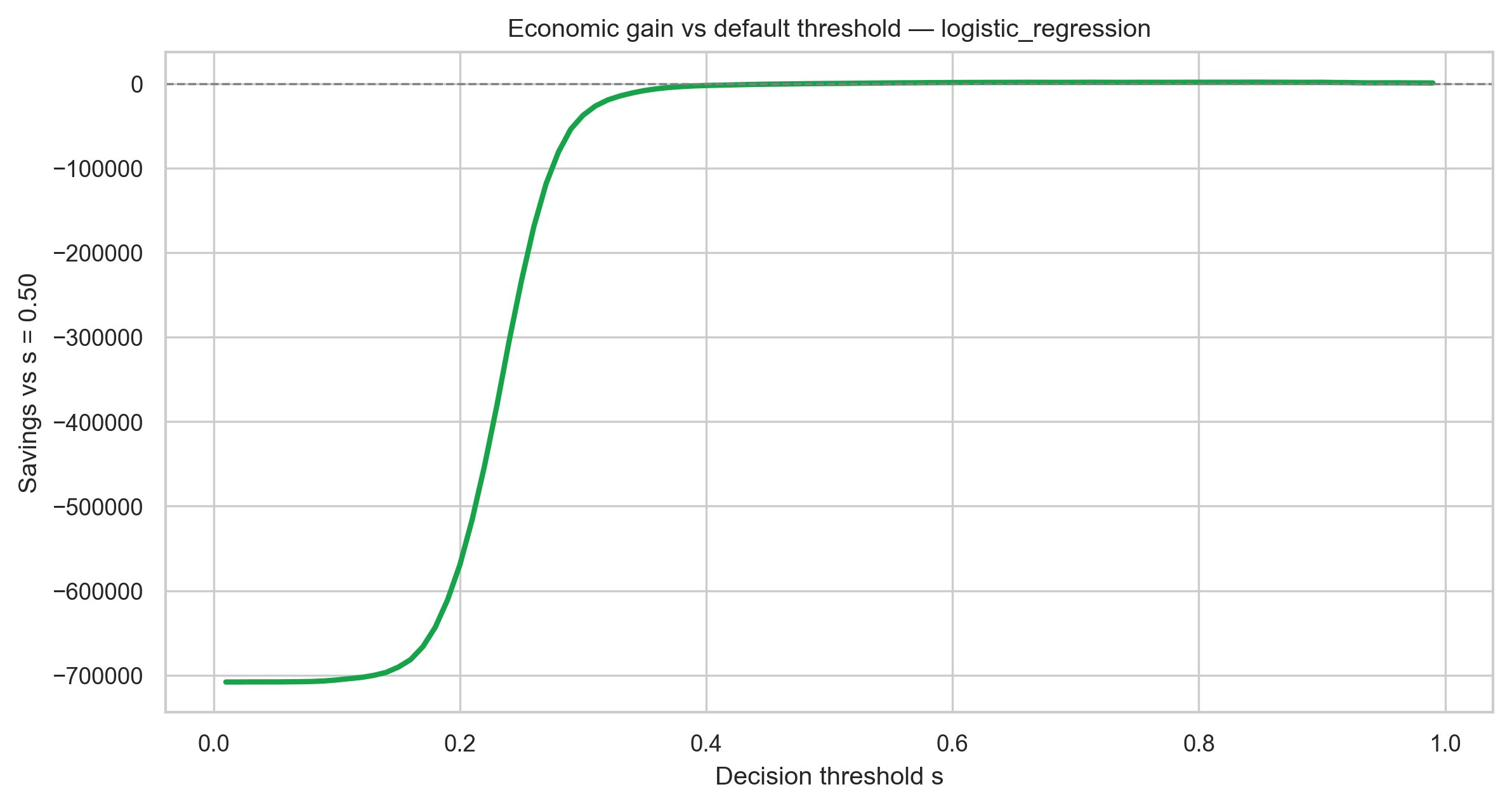
\includegraphics[width=0.92\textwidth]{figures/image35.png}
\end{figure}

\emph{Gains économiques — Régression Logistique.}

\section{Annexe C — Tableau de bord Power BI — Toutes les pages}

Les neuf captures suivantes présentent l'intégralité du tableau de bord Power BI développé dans le cadre de ce mémoire. Toutes les données affichées dans ce tableau de bord sont des données synthétiques générées pour la démonstration opérationnelle du prototype, sauf les métriques de benchmark (pages 5, 6, 7) qui proviennent des fichiers CSV d'export du pipeline d'apprentissage sur le dataset ULB.

\begin{figure}[H]
\centering
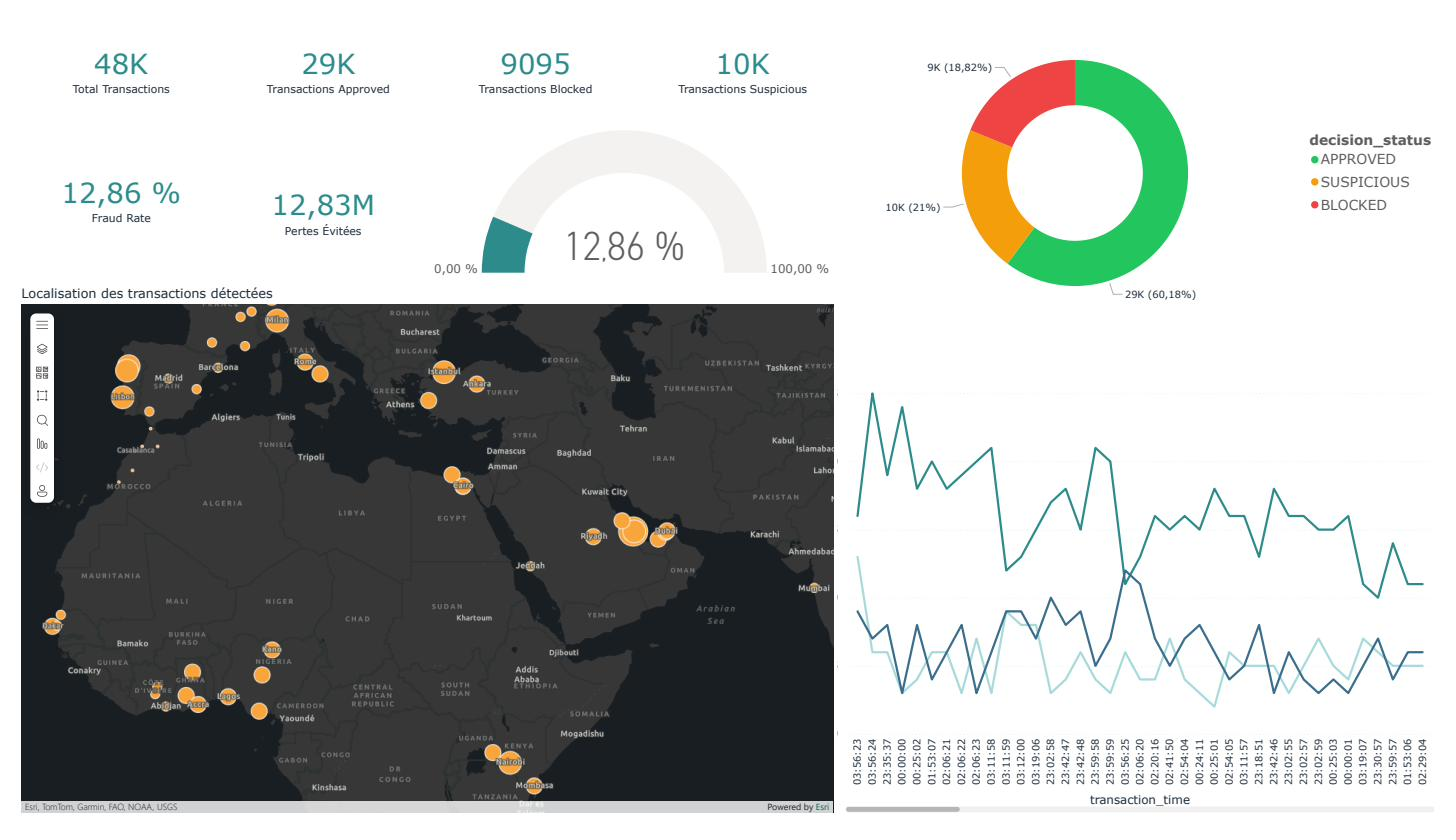
\includegraphics[width=0.92\textwidth]{figures/image36.jpg}
\end{figure}

\emph{Dashboard Power BI — Vue exécutive — Volume de transactions, taux de fraude, répartition des décisions, pertes évitées. Données de simulation synthétiques (sauf métriques benchmark pages 5–7 issues du }\emph{dataset}\emph{ ULB).}

\begin{figure}[H]
\centering
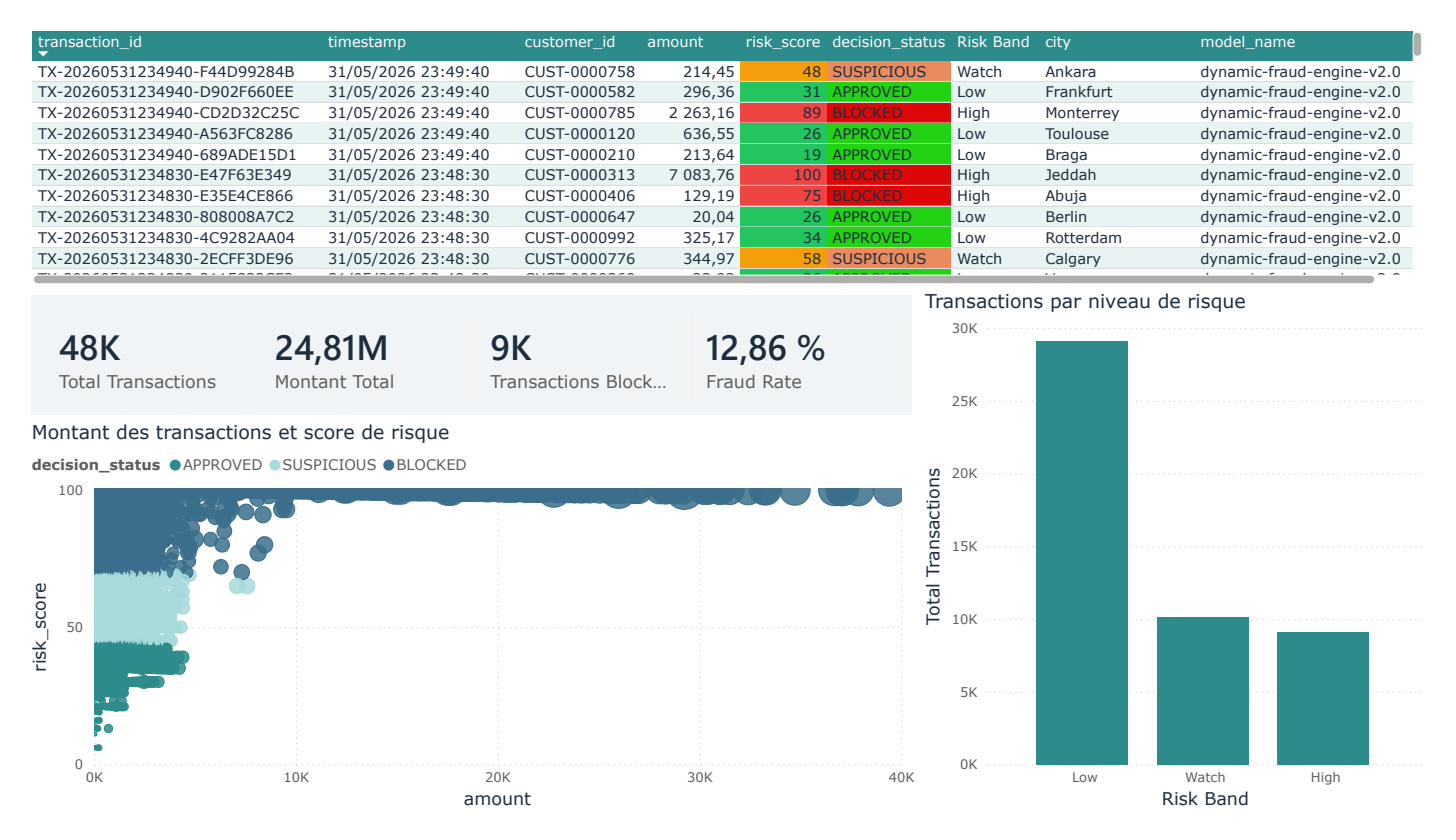
\includegraphics[width=0.92\textwidth]{figures/image37.jpg}
\end{figure}

\emph{Dashboard Power BI — Transactions en temps réel — Flux live, score de risque, décision par transaction. Données de simulation synthétiques (sauf métriques benchmark pages 5–7 issues du }\emph{dataset}\emph{ ULB).}

\begin{figure}[H]
\centering
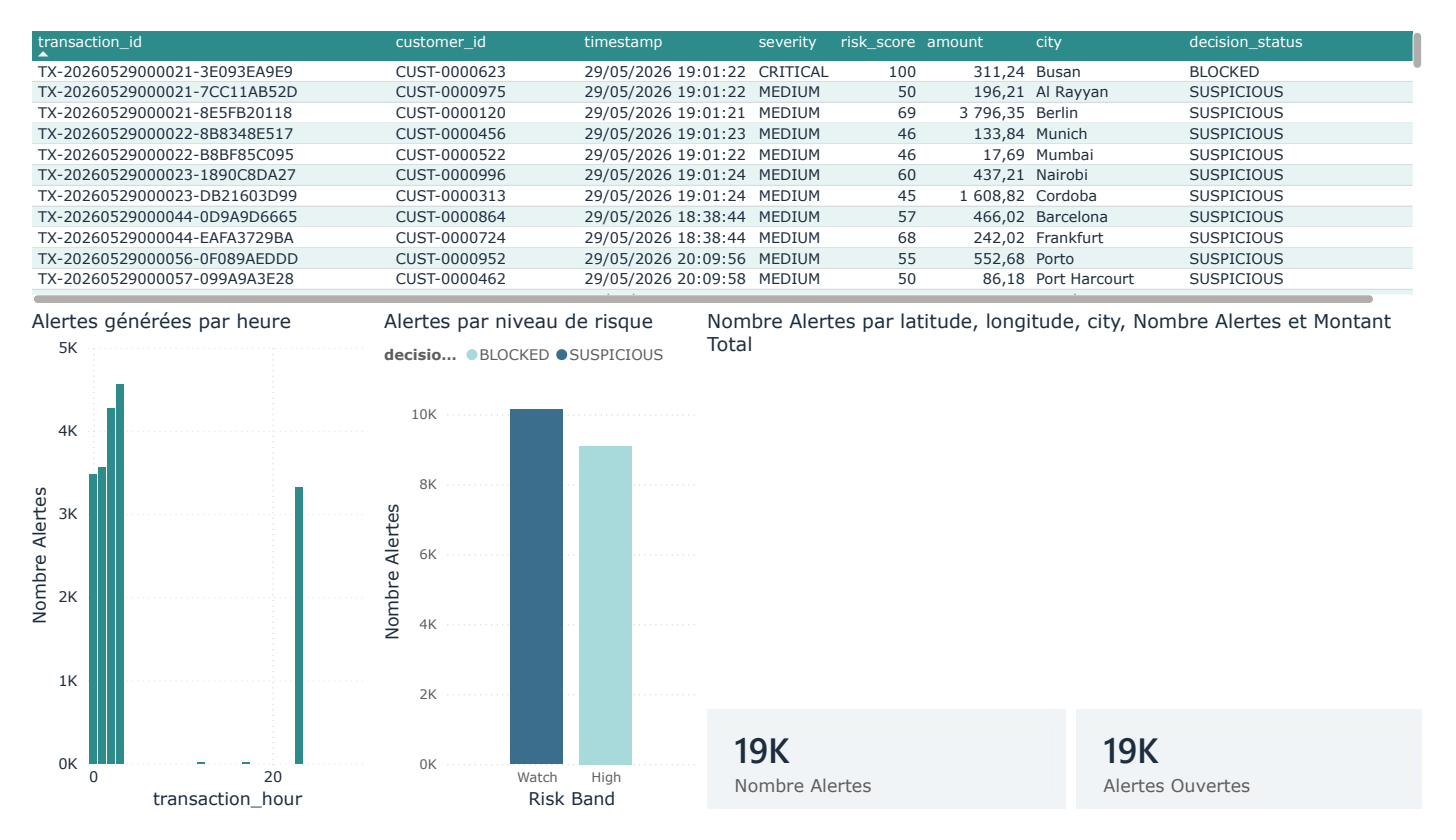
\includegraphics[width=0.92\textwidth]{figures/image38.jpg}
\end{figure}

\emph{Dashboard Power BI — Alertes — Volume, répartition par niveau de risque, liste détaillée des alertes. Données de simulation synthétiques (sauf métriques benchmark pages 5–7 issues du }\emph{dataset}\emph{ ULB).}

\begin{figure}[H]
\centering
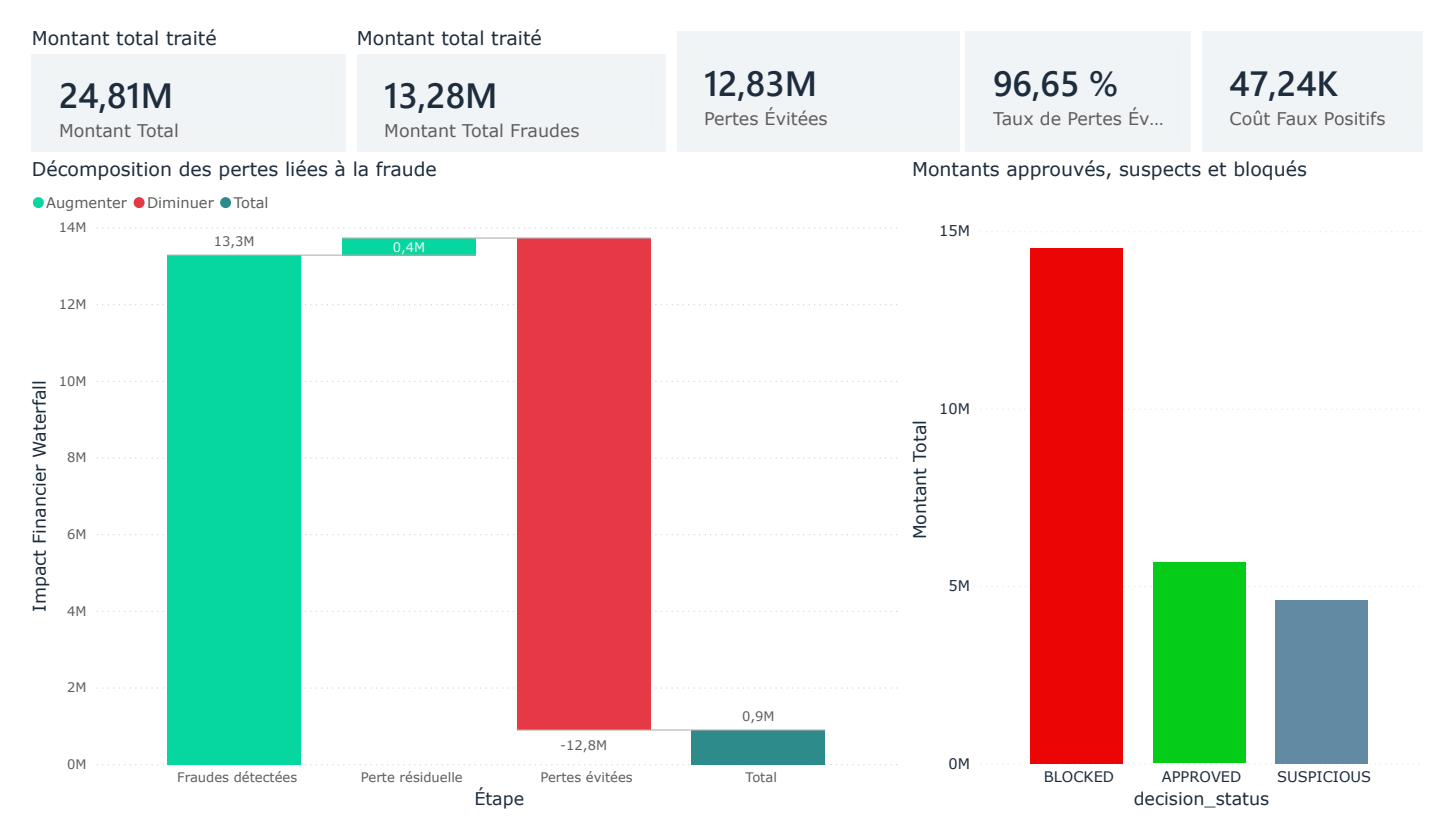
\includegraphics[width=0.92\textwidth]{figures/image39.jpg}
\end{figure}

\emph{Dashboard Power BI — Analyse financière — Montants traités, pertes évitées, décomposition }\emph{waterfall}\emph{. Données de simulation synthétiques (sauf métriques benchmark pages 5–7 issues du }\emph{dataset}\emph{ ULB).}

\begin{figure}[H]
\centering
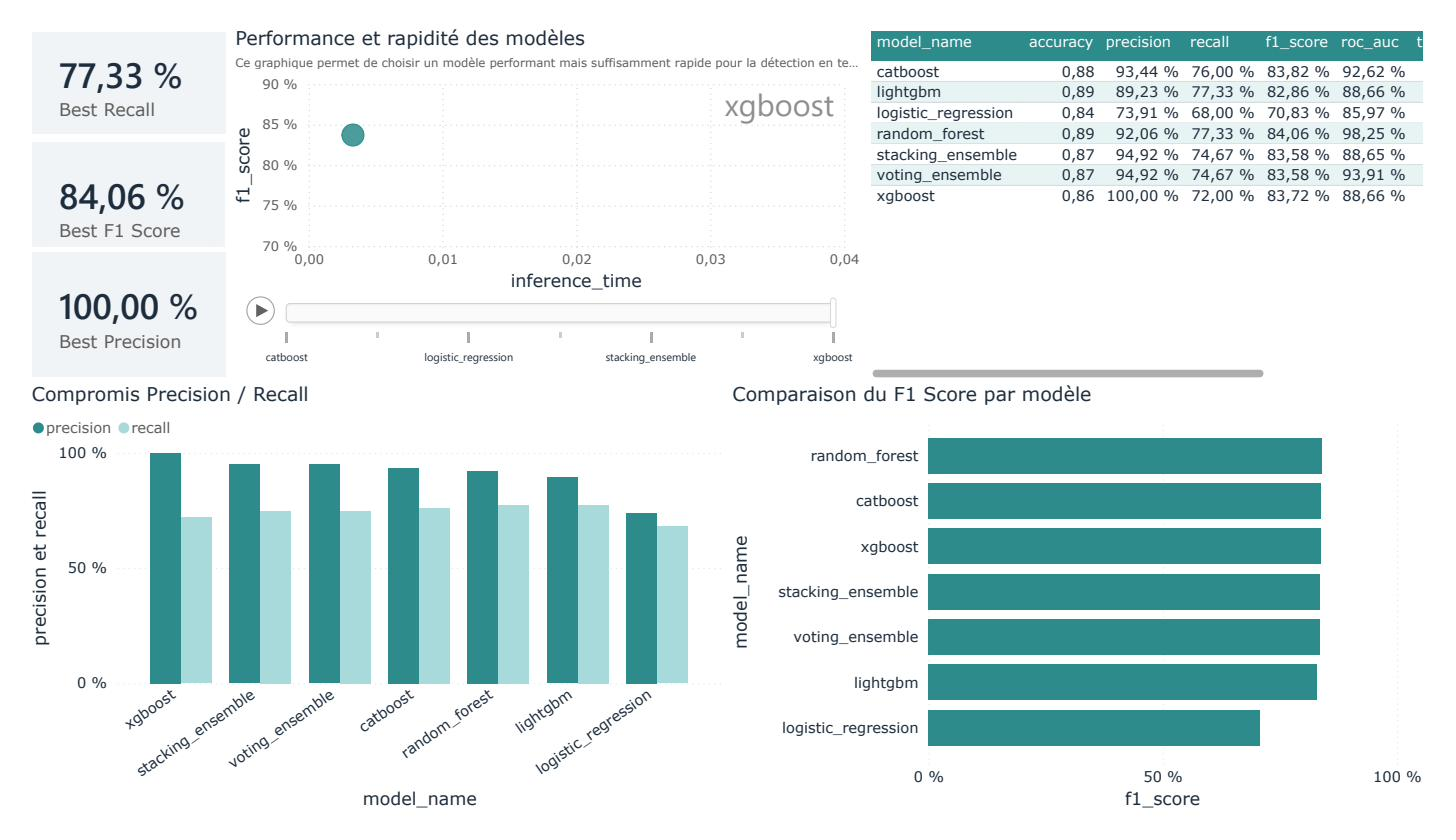
\includegraphics[width=0.92\textwidth]{figures/image40.jpg}
\end{figure}

\emph{Dashboard Power BI — Benchmark des modèles — F1, précision, rappel, comparaison vitesse/performance. Données de simulation synthétiques (sauf métriques benchmark pages 5–7 issues du }\emph{dataset}\emph{ ULB).}

\begin{figure}[H]
\centering
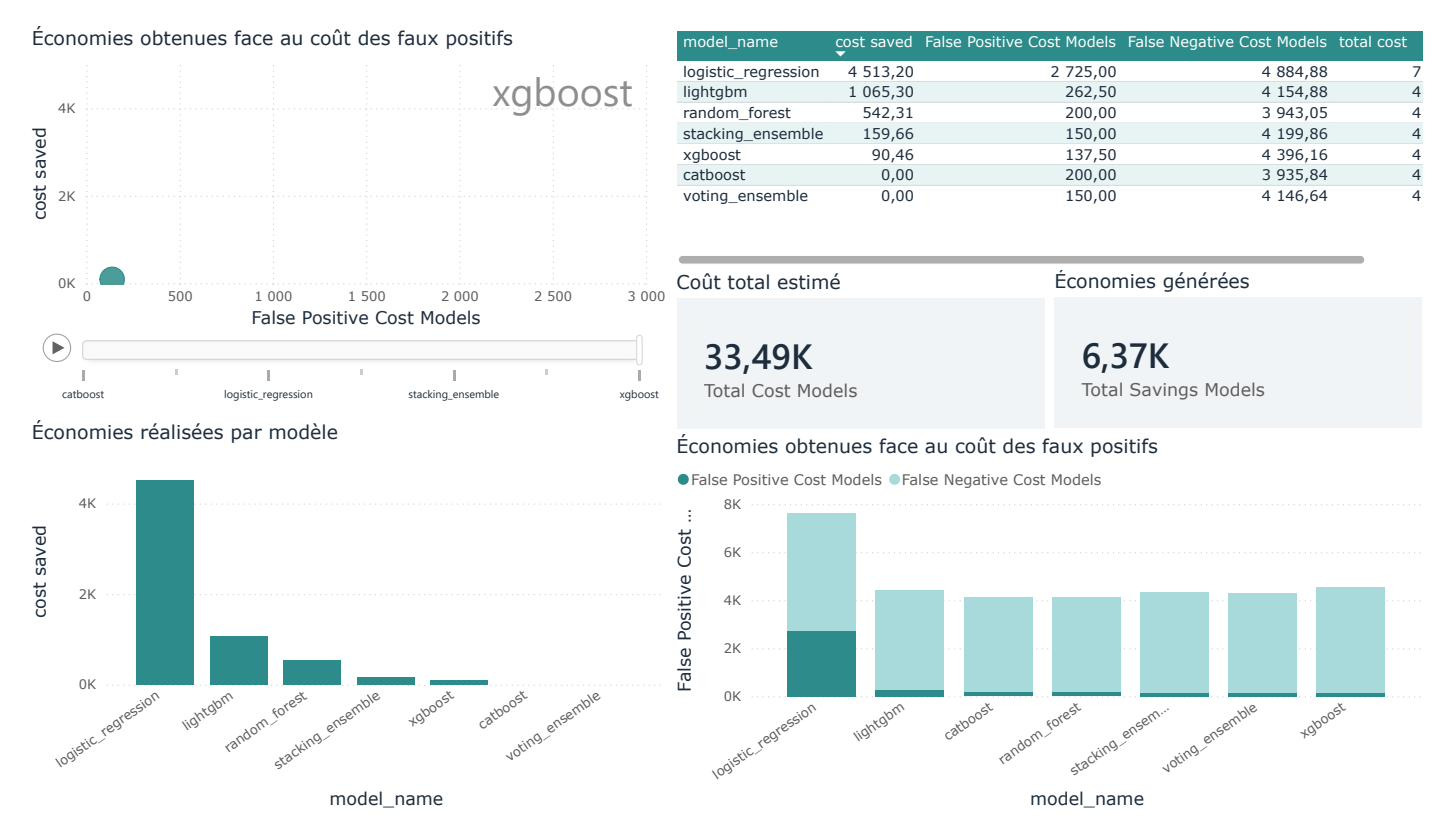
\includegraphics[width=0.92\textwidth]{figures/image41.jpg}
\end{figure}

\emph{Dashboard Power BI — Analyse des coûts — Économies par modèle, décomposition FP/FN. Données de simulation synthétiques (sauf métriques benchmark pages 5–7 issues du }\emph{dataset}\emph{ ULB).}

\begin{figure}[H]
\centering
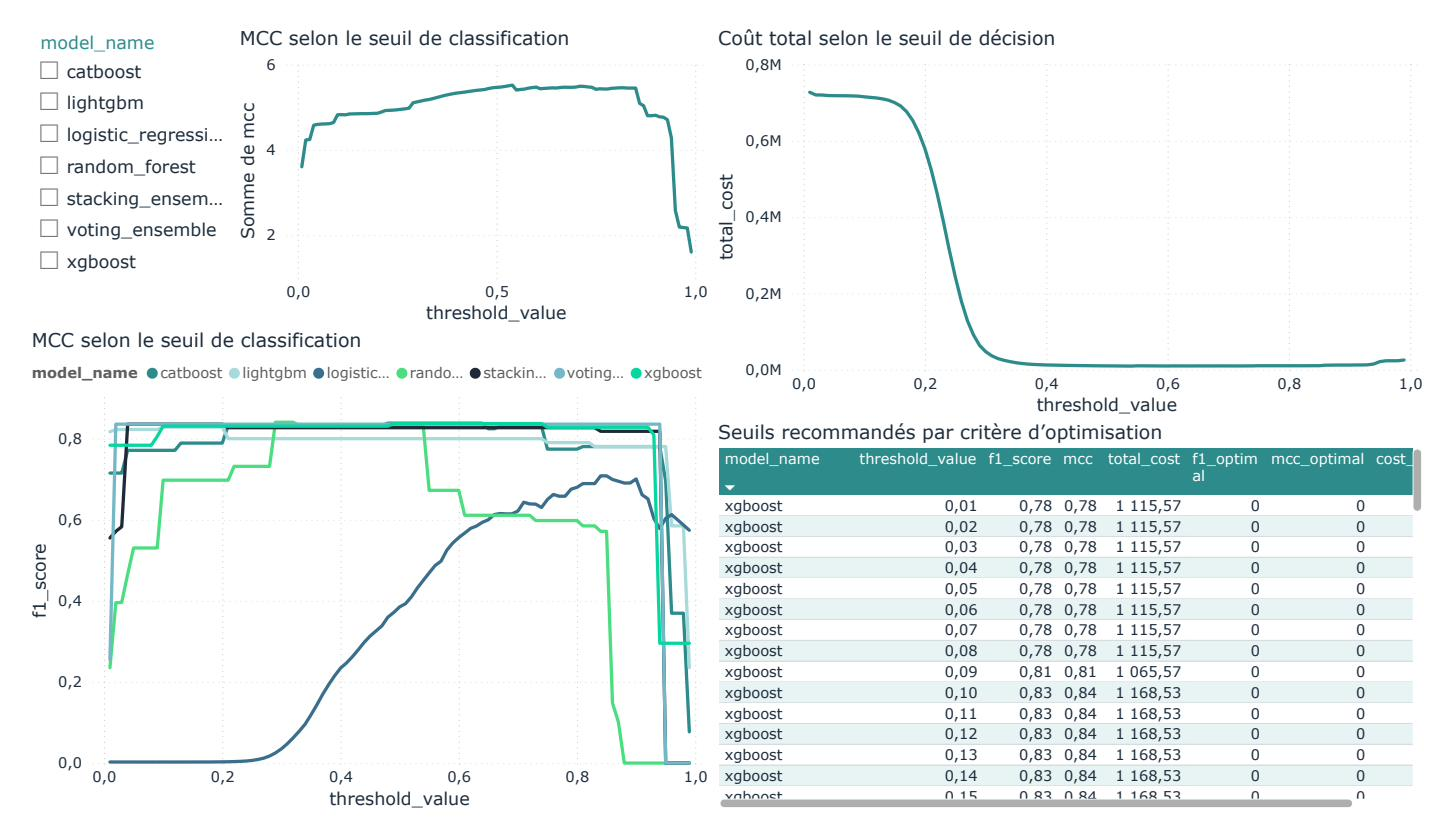
\includegraphics[width=0.92\textwidth]{figures/image42.jpg}
\end{figure}

\emph{Dashboard Power BI — Optimisation du seuil — MCC et coût total par seuil, seuils recommandés. Données de simulation synthétiques (sauf métriques benchmark pages 5–7 issues du }\emph{dataset}\emph{ ULB).}

\begin{figure}[H]
\centering
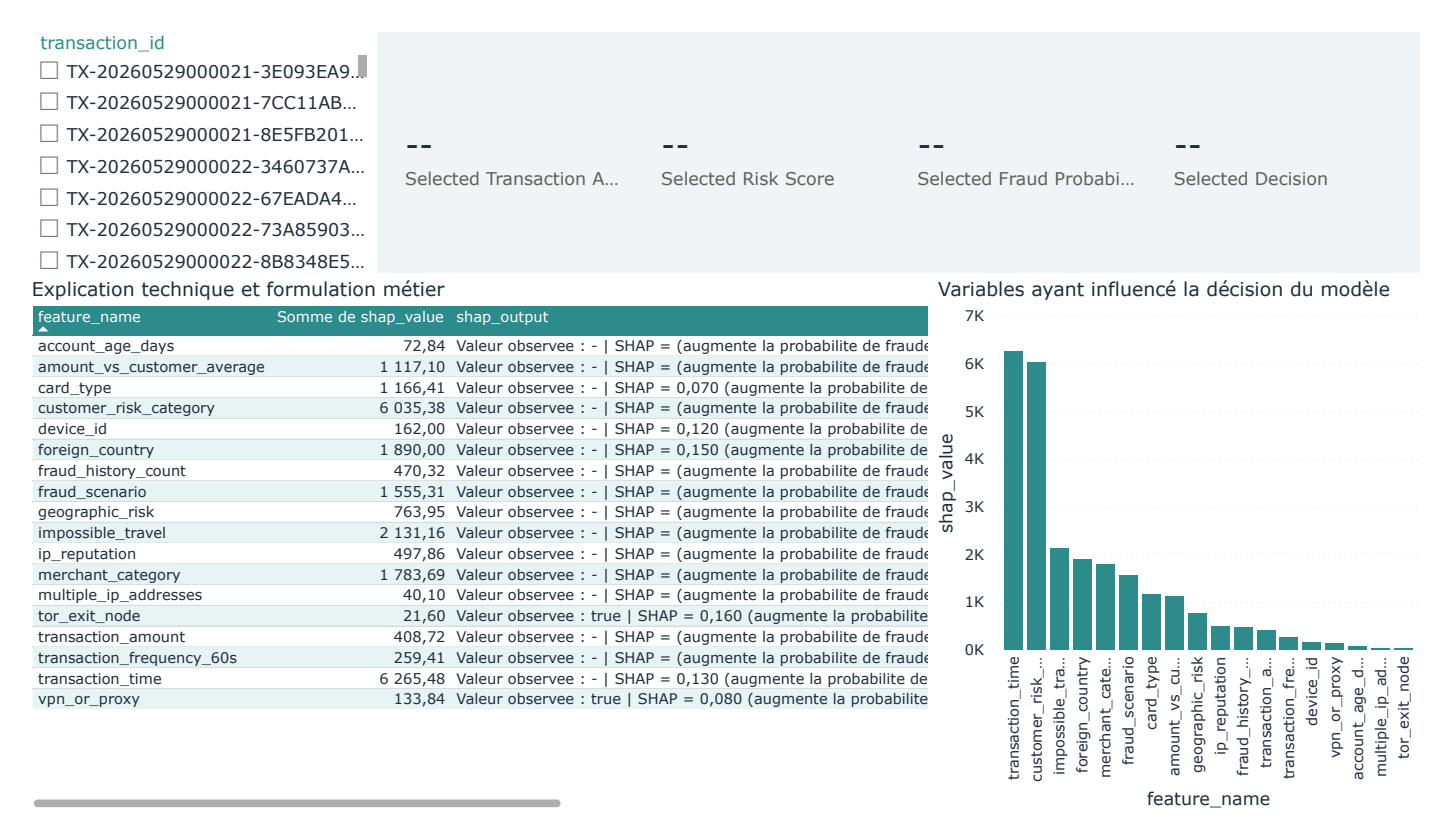
\includegraphics[width=0.92\textwidth]{figures/image43.jpg}
\end{figure}

\emph{Dashboard Power BI — Explicabilité SHAP — Variables influentes par transaction, fiches d'explication. Données de simulation synthétiques (sauf métriques benchmark pages 5–7 issues du }\emph{dataset}\emph{ ULB).}

\begin{figure}[H]
\centering
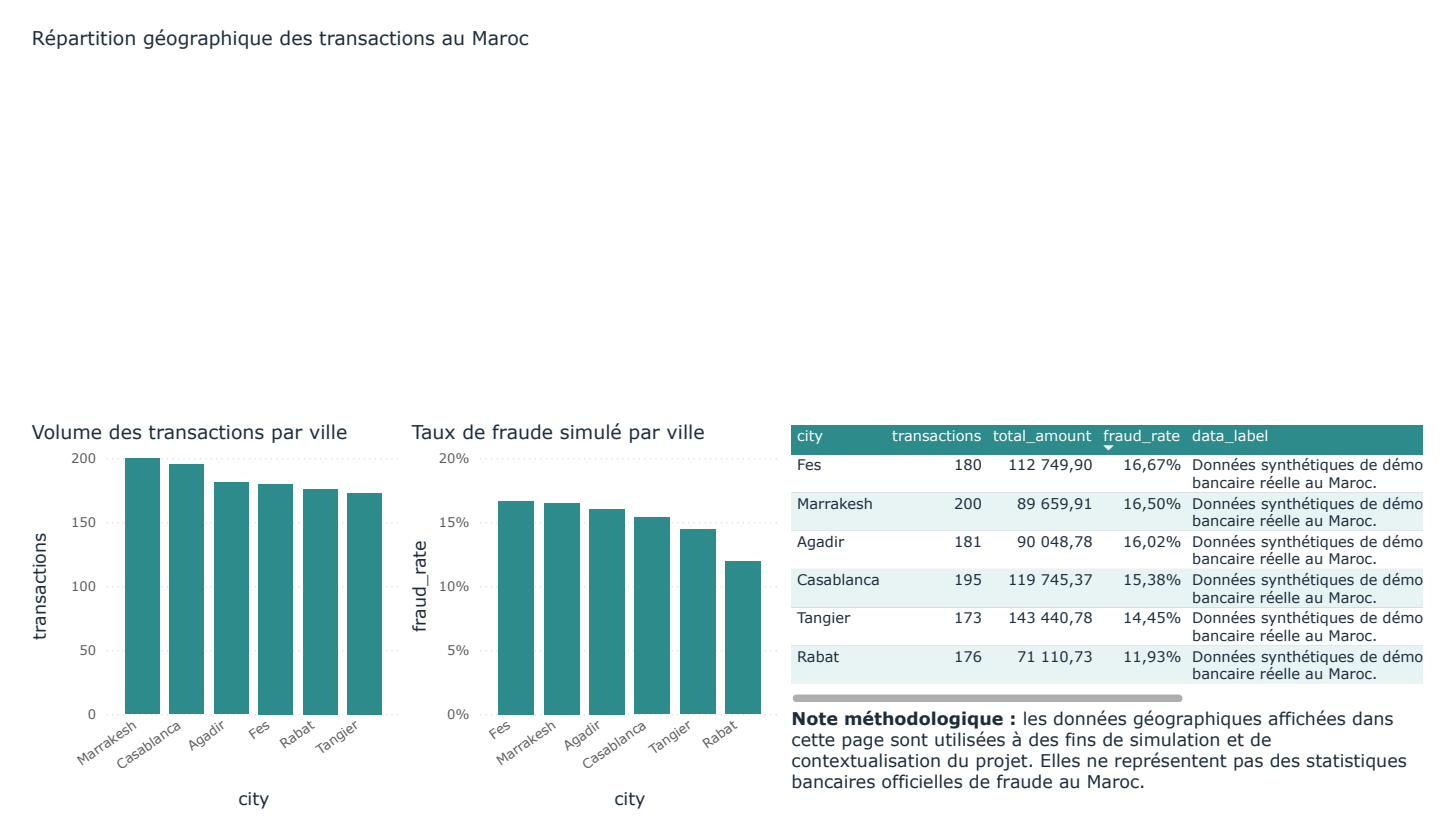
\includegraphics[width=0.92\textwidth]{figures/image44.jpg}
\end{figure}

\emph{Dashboard Power BI — Contexte marocain — Distribution géographique simulée (données synthétiques). Données de simulation synthétiques (sauf métriques benchmark pages 5–7 issues du }\emph{dataset}\emph{ ULB).}

\section{Annexe D — Hyper-paramètres retenus par modèle}

\begin{longtable}{|p{0.225\textwidth}|p{0.225\textwidth}|p{0.225\textwidth}|p{0.225\textwidth}|}
\hline
Modèle & Paramètre & Valeur & Justification \\
\hline
\endfirsthead
\hline
Modèle & Paramètre & Valeur & Justification \\
\hline
\endhead
XGBoost & n\_estimators & 300 & Convergence stable sans surapprentissage \\
\hline
XGBoost & learning\_rate & 0,05 & Apprentissage lent pour meilleure généralisation \\
\hline
XGBoost & max\_depth & 6 & Équilibre profondeur/surapprentissage \\
\hline
XGBoost & scale\_pos\_weight & 567,9 & Ratio négatifs/positifs sur jeu d'entraînement \\
\hline
Random Forest & n\_estimators & 200 & Stabilité de l'agrégation \\
\hline
Random Forest & max\_depth & 10 & Contrôle du surapprentissage \\
\hline
Random Forest & class\_weight & 'balanced' & Pondération aux fréquences inverses \\
\hline
LightGBM & num\_leaves & 63 & Complexité modérée leaf-wise \\
\hline
LightGBM & min\_child\_samples & 20 & Régularisation minimale \\
\hline
CatBoost & depth & 6 & Profondeur standard données tabulaires \\
\hline
CatBoost & l2\_leaf\_reg & 3,0 & Régularisation L2 \\
\hline
Régression Logistique & C & 0,1 & Forte régularisation pour données déséquilibrées \\
\hline
\end{longtable}

\section{Annexe E — Note méthodologique sur la perspective marocaine}

L'ensemble des analyses et recommandations relatives au contexte marocain reposent sur des sources documentaires institutionnelles vérifiées (BAM, CMI, HCP, ONMT) et sur des hypothèses de transposition analytique. Aucune ne constitue une validation empirique sur des données bancaires marocaines réelles. La validation opérationnelle nécessiterait : (1) un dataset local représentatif, anonymisé, sécurisé, conforme à la Loi 09-08 ; (2) validation des paramètres de coût auprès d'établissements bancaires marocains ; (3) consultation de la CNDP ; (4) autorisations réglementaires de Bank Al-Maghrib
